\section{Appendix}
%\subsection{Theoretical model}
%\label{sec:appendix_wildland__theoretical}
%\subsubsection{Vegetation dynamics}
%In cell $i$ at time $t$, vegetation ages $A_i(t)$ evolves according to the following :
%\begin{equation}
%    A_i(t+1) = (A_i(t) + 1)(1-x_i(t)), t\in \{0,1,..., T\}, \forall i \in C
%\label{eq:fuel_dyn}
%\end{equation}
%Where $x_i(t)\in \{0,1\}$ is a binary variable, representing the treatment status of cell $i$ at time $t$. Correspondingly, the age vector across the landscape is $A(t)=\{A_i(t)\}_{i\in C}$.

%\subsubsection{Mature habitat and risky patch designation}
%Cell $i$ is labeled 'mature' to host wildlife in year $t$ as:
%\begin{equation}
%    Mature_i\left(A(t)\right) = \begin{cases}
%        1 &\text{ if } A_i(t) \geq m\\
%        0 &\text{ otherwise }
%    \end{cases}
%\label{eq:mature}
%\end{equation}
%Where $m$ is the 'mature' threshold. Correspondingly, the vector of mature cells across the landscape is $Mature\left(A(t)\right)=\{Mature_i\left(A(t)\right)\}_{i\in C}$

%Similarly, cell $i$ is labeled as 'high fuel load' in year $t$ as:
%\begin{equation}
%    High_i\left(A(t)\right) = \begin{cases}
%1 &\text{ if } A_i(t)\geq d\\
%0 &\text{ otherwise}
%    \end{cases}
%\label{eq:high_fuel}
%\end{equation}
%Where $d$ is the 'high fuel load' threshold. Correspondingly, the vector of high fuel load cells across the landscape is $High\left(A(t)\right)=\{High_i\left(A(t)\right)\}_{i\in C}$

%We assume that the maturity threshold is crossed before the high risk threshold, i.e $m<d$.

\subsection{Global connectivity index and graph theory}

\label{sec:connectivity}

%Let a grided landscape of size $n$, where for each cell $a_i$ in the set of cells $\mathcal{A}$ in the landscape, one defines $\Phi_i$ the set of cells connected to cell $i$ (i.e, cells share the same status and can only be in the 8-direction direct neighborhood). Moreover, let $Q_{ij}$ be a binary variable such that $Q_{ij}=1$ if cells $a_i$ and $a_j$ are connected, $0$ otherwise.

\cite{minas_spatial_2014} work with a collection of cells $I$. This landscape can be represented by a graph structure $\mathcal{G}=(\mathcal{V}, \mathcal{E})$.
For each $v_i \in \mathcal{V}$, define a neighborhood\footnote{Notice that \textit{belonging to the neighborhood of} is a symmetric binary relationship e.g. if $v_i \in \Phi_j \iff v_j \in \Phi_i$, as we are working with undirected graphs} of $v_i$ by $\Phi_i = \{ v_j \text{ such that } (v_j, v_i) \in \mathcal{E} \}$. 
Finally, let $Q_{ij} \in \{0,1\}$ where $Q_{ij}=1$ if $v_i$ and $v_j$ are connected. \cite{minas_spatial_2014} define the following connectivity metric over a landscape: 

\begin{equation}
    z^*_t = \sum_{i \in I}\sum_{j \in \Phi_i}Q_{ij}
    \label{eq:obj_minas}
\end{equation}

%Now view the landscape as a graph $G$, with vertices $V$ and edges $E$ such that $G(V,E)$. 
For the proof, assume $Y \in \{0,1\}^{n^2}$ such that $Y_i=1$ if cell $i$ is 'high risk' and $0$ otherwise, and that we focus on the high risk graph on the landscape. The argument is identical in the case of mature habitat. 

In graph theory, an adjacency matrix $\mathcal{K}$ for an undirected graph is a binary, symmetric, square matrix of dimension $\mathrm{card}(V)^2$ where $k_{ij}=1$ if vertices $i$ and $j$ are connected, $0$ otherwise. In our context, it is clear that $k_{ij}=Q_{ij}$. Equation \ref{eq:obj_minas} can be reformulated as : 
\begin{align*}
    Y' \mathcal{K} Y &= \sum_j\left( Y_j \sum_i Y_i k_{ij}\right)\\
    &= \sum_j \sum_i \left( Y_j Y_i k_{ij}\right)
\end{align*}
And notice that $Y_j Y_i k_{ij} = Q_{ij}$, so :

\begin{align*}
    Y' \mathcal{K} Y &=\sum_{i \in I}\sum_{j \in \Phi_i}Q_{ij}\\
					 &= \sum_j\left( Y_j \left( Y_j k_{jj} + \sum_{i \neq j}Y_i k_{ij}\right)\right)
\end{align*}
Given the symmetric nature of $\mathcal{K}$, $\forall i \neq j$, $k_{ij}=k_{ji}$. Each cell is connected to itself so $k_{jj}=1$. Additionally, as $Y_i\in\{0,1\}$ then $Y_i^2 \in \{0,1\}$:
\begin{align*}
    Y'\mathcal{K} Y & =\sum_j \left(Y_j^2 + \sum_{i\neq j}Y_i Y_j k_{ij}\right)\\ 
          & = \sum_j Y_j + \sum_{j} \left(\sum_{i \neq j }Y_j Y_i k_{ij}\right)   \\
          & = \sum_j Y_j + \sum_{j} d_{j}
\end{align*}

The first sum is the number of high risk cells, i.e. $\mathrm{card}(\mathcal{V})$. 
In the second sum, $\sum_{i \neq j} Y_j Y_i a_{ij}$ is the degree of each vertex $j$ excluding self loops. In a graph with no self loops, by definition, $\sum_{j} d_j = \mathrm{card}(\mathcal{E})$.
%In the second sum, $\sum_{i \neq j} Y_j Y_i a_{ij}$ is the number of connections of cell $i$ to cell $j$, as the product $Y_i Y_j k_{ij}=1$ if and only if cell $i$ and $j$ share the same status ($Y_i = Y_j$) and are in the 8-cell neighborhood ($k_{ij}=1)$. By definition, the sum of the number of connections of each cell to other cells is $card(E)$. 

Hence, for a set of cells $I$ reformulated in terms of graph theory : 
\begin{equation}
        \sum_{i \in I}\sum_{j \in \Phi_i}Q_{ij} = \mathrm{card}(V) + 2 \mathrm{card}(E)
\end{equation}

\begin{figure}[H]
    \centering
    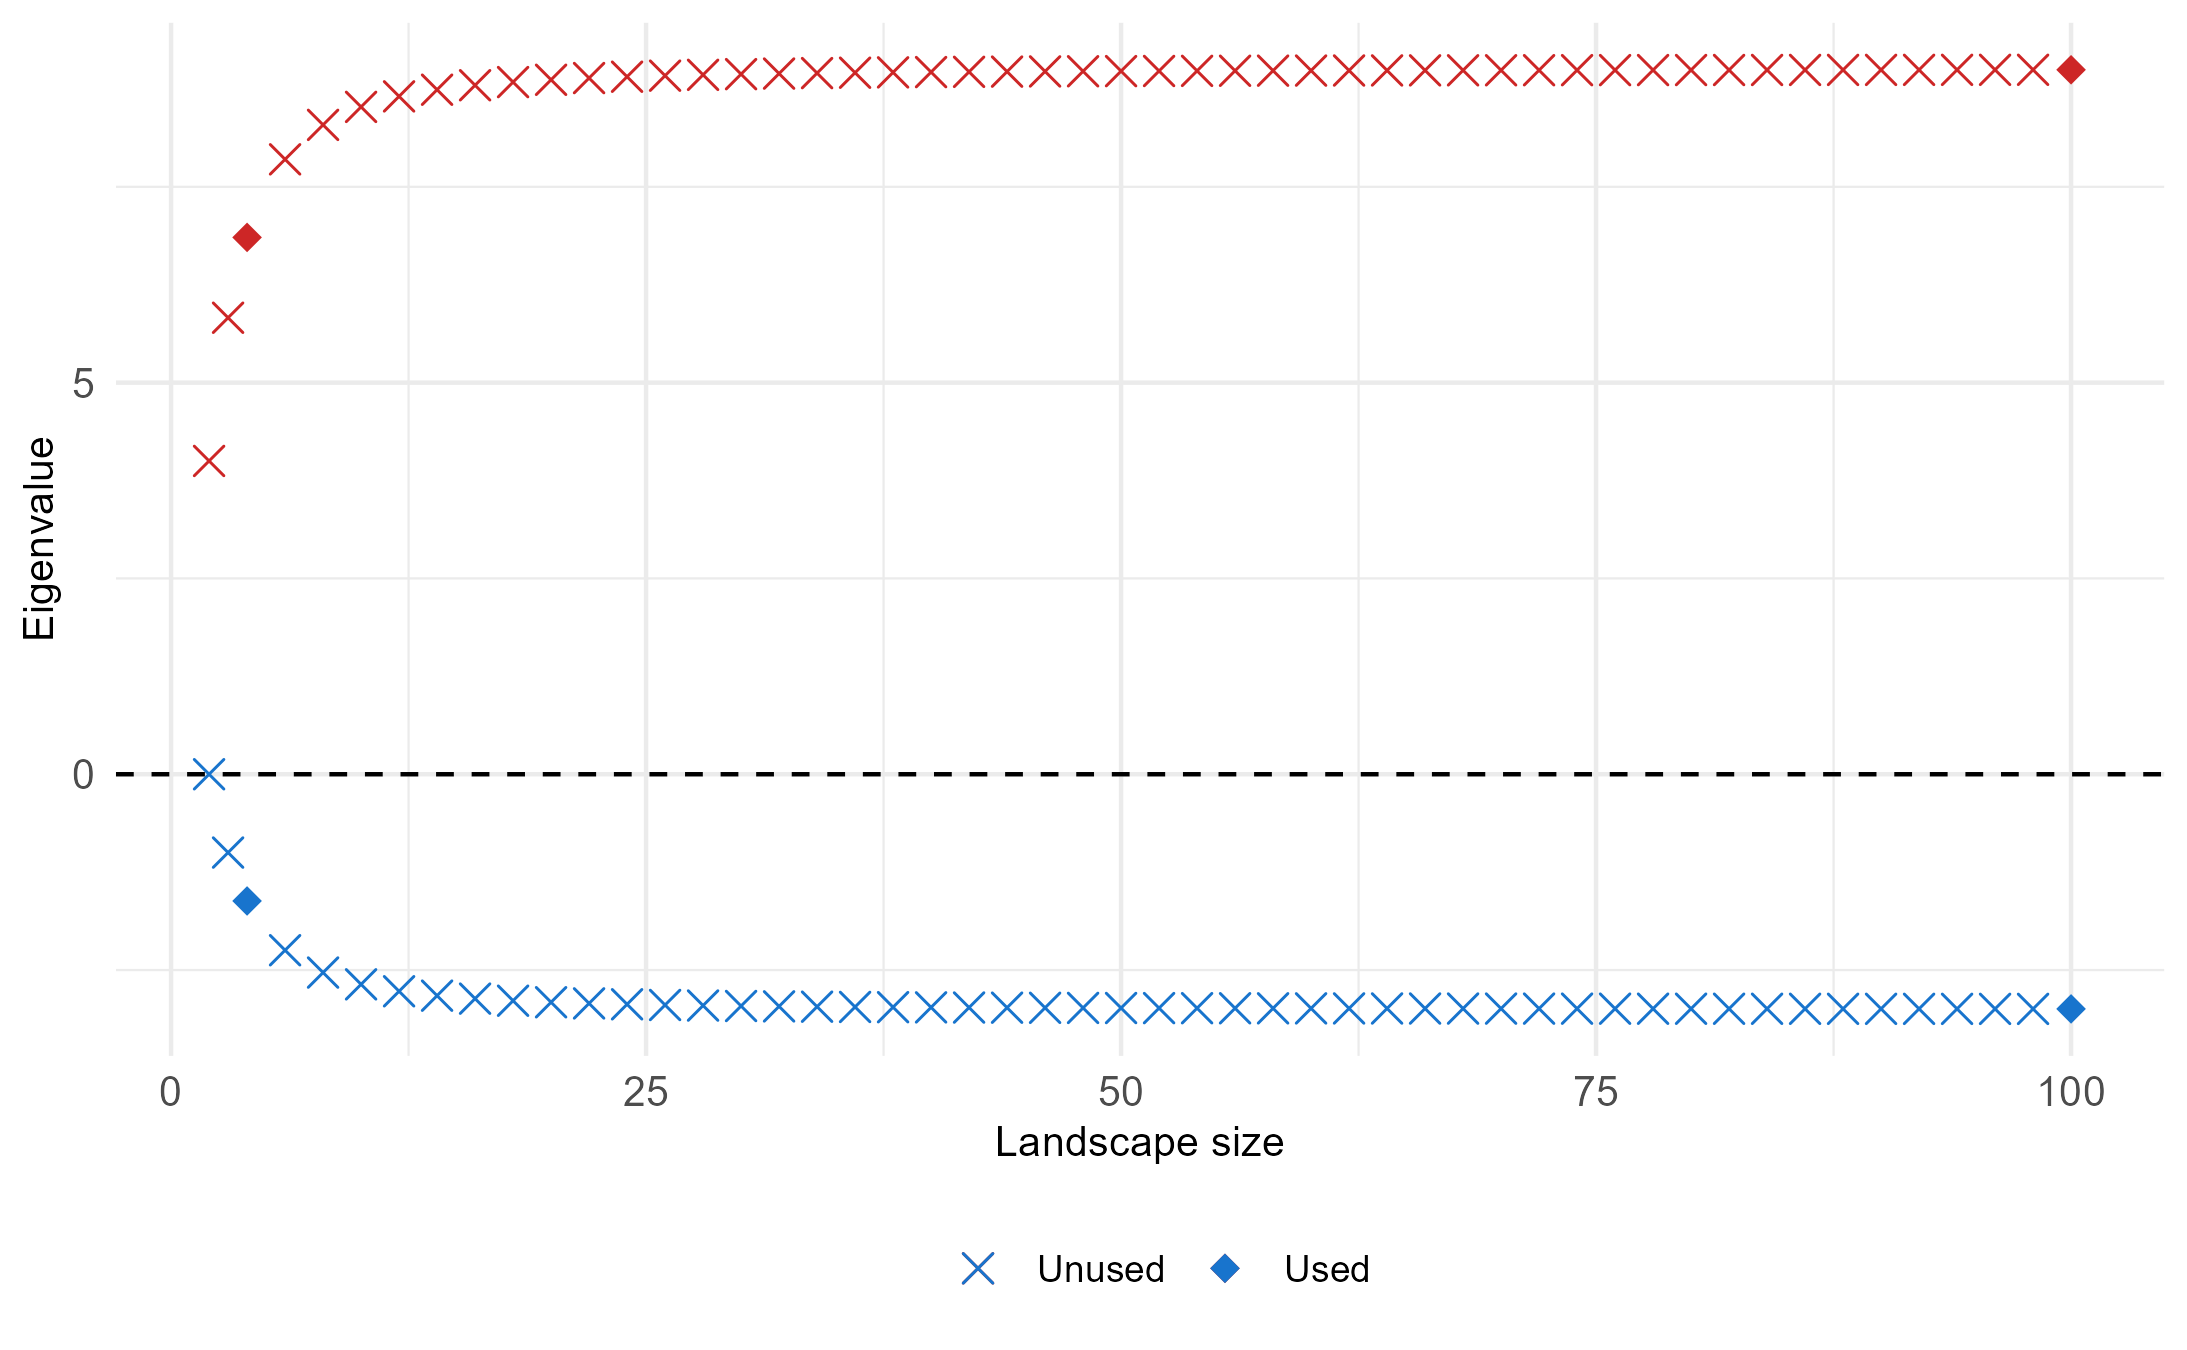
\includegraphics[width=0.8\linewidth]{figures/wildland/eigenvalues.png}
    \caption{Maximum and minimum eigenvalues of $\mathcal{K}$ depending on graph size}
    \subcaption*{In red, the maximum eigenvalues, in blue, the minimal eigenvalues. Diamond-shaped points represent values actually used for the present study. Dotted line at 0}
    \label{fig:eigenvalues}
\end{figure}




%The Bellman equation links current and future payoffs in a recurring fashion.
%\begin{equation}
%    V(t,A)= \min_{x\in\{0,1\}^{n^2}} \left(H(A) + V(t+1, A_t+1)\right)
%\end{equation}
%subject to constraints (\ref{const:dyn}), (\ref{const:budget}), (\ref{constr:biod}) and (\ref{const:control}). 

%We use backward induction given by the final value $ V(T, A) = H(A)$ to dynamically solve the program. 

%\subsubsection{Decision-making under uncertainty and constrained optimization}

%Let $A_t$ be represented by its habitat graph $G_B = (V_B, E_B)$, and its high-risk graph $G_E = (V_F, E_F)$. Let $G_{\Tilde{B}} = (V_{\Tilde{B}}, E_{\Tilde{B}})$ be the graph of the remaining habitat, such that : 
%\begin{align*}
%    V_{\tilde{B}} &= V_B \setminus V_F\\
%    E_{\tilde{B}} &= E_{B} \setminus ( E_{F} \cup E_{B\cap F})
%\end{align*}
%Where $E_{B \cap F}$ is the set of vertices connecting nodes from the habitat graph to the high-risk graph. Let $A'$ be the corresponding land vector such that if $a_i =2$ before fire, then $a'_i=0$ after fire. Eventually, assume that ignition follows a Bernoulli process and is independent of the landscape's measured properties such that $\mathcal{I} \sim \mathcal{B}(p)$.\\

%In the case fire ignites in period $t$, habitat burns and connectivity is degraded, and the payoff is $H_B(A'_t) = card(V_{\Tilde{B}}) + 2card(E_{\Tilde{B}})$. On the other hand, if fire does not ignite, the payoff is $H_B(A)$. The expected payoff is :
%$$E=p H_B(A'_t) + (1-p) H_B(A_t)$$
%Given that $E_{B\cap F} \neq \emptyset$, notice that :
%\begin{align*}
%    H_B(A'_t) &= card(V_{\Tilde{B}}) + 2card(E_{\Tilde{B}})\\
%    & = card(V_B\setminus V_F) + 2card\left(E_B \setminus (E_F \cup E_{B\cap F})\right)\\
%    & = card(V_B) - card(V_F) + 2 card(E_B) - 2 card(E_F) - 2 card (E_{B\cap F})\\
%    & = H_B(A_t)-H_F(A_t) - 2 card(E_{B\cap F})\\
%    & \leq H_B(A_t) - H_F(A_t)
%\end{align*}
%Hence : 
%\begin{align*}
%   & E \leq E' = p(H_B(A_t) - H_F(A_t)) + (1-p) H_B(A_t) \\
%    \Rightarrow & E \leq  H_B(A_t) - pH_F(A_t) \\
%    \Rightarrow &  - E \geq p H_F(A_t) - H_B(A_t)
%\end{align*}

%\textbf{Clarify the expected damage thing, it's unclear as of now. }
%Myabe say that if $E'>E$ and we minimize $-E'$ we do something lower than E? Minimize a lower bound of expected utility? Unclear with the minus sign...
\subsection{Large scale landscape characteristics}

\begin{table}[H]
\centering
\begin{tabular}{|ccc||c|}
\hline
 & Age classes &  & Autocorrelation \\
\hline
\textit{Juvenile}& \textit{Adolescent}& \textit{Mature}& \\
\hline
33\% & 33\% & 34\% & 0.5 \\
10\% & 45\% & 45\% & 0.7 \\
10\% & 10\% & 80\% & 0.9 \\
10\% & 80\% & 10\% & 1.3 \\
& & & 1.8\\
\hline
\end{tabular}
\caption{Summary of the large scale simulated landscapes characteristics}
\subcaption*{For each distribution profile governing the number of cells in a landscape, all of the spatial autocorrelation values are applied making $4\times 5$ landscapes}
\label{tab:composition_nlm}
\end{table}
\clearpage

\begin{figure}[H]
    \centering
    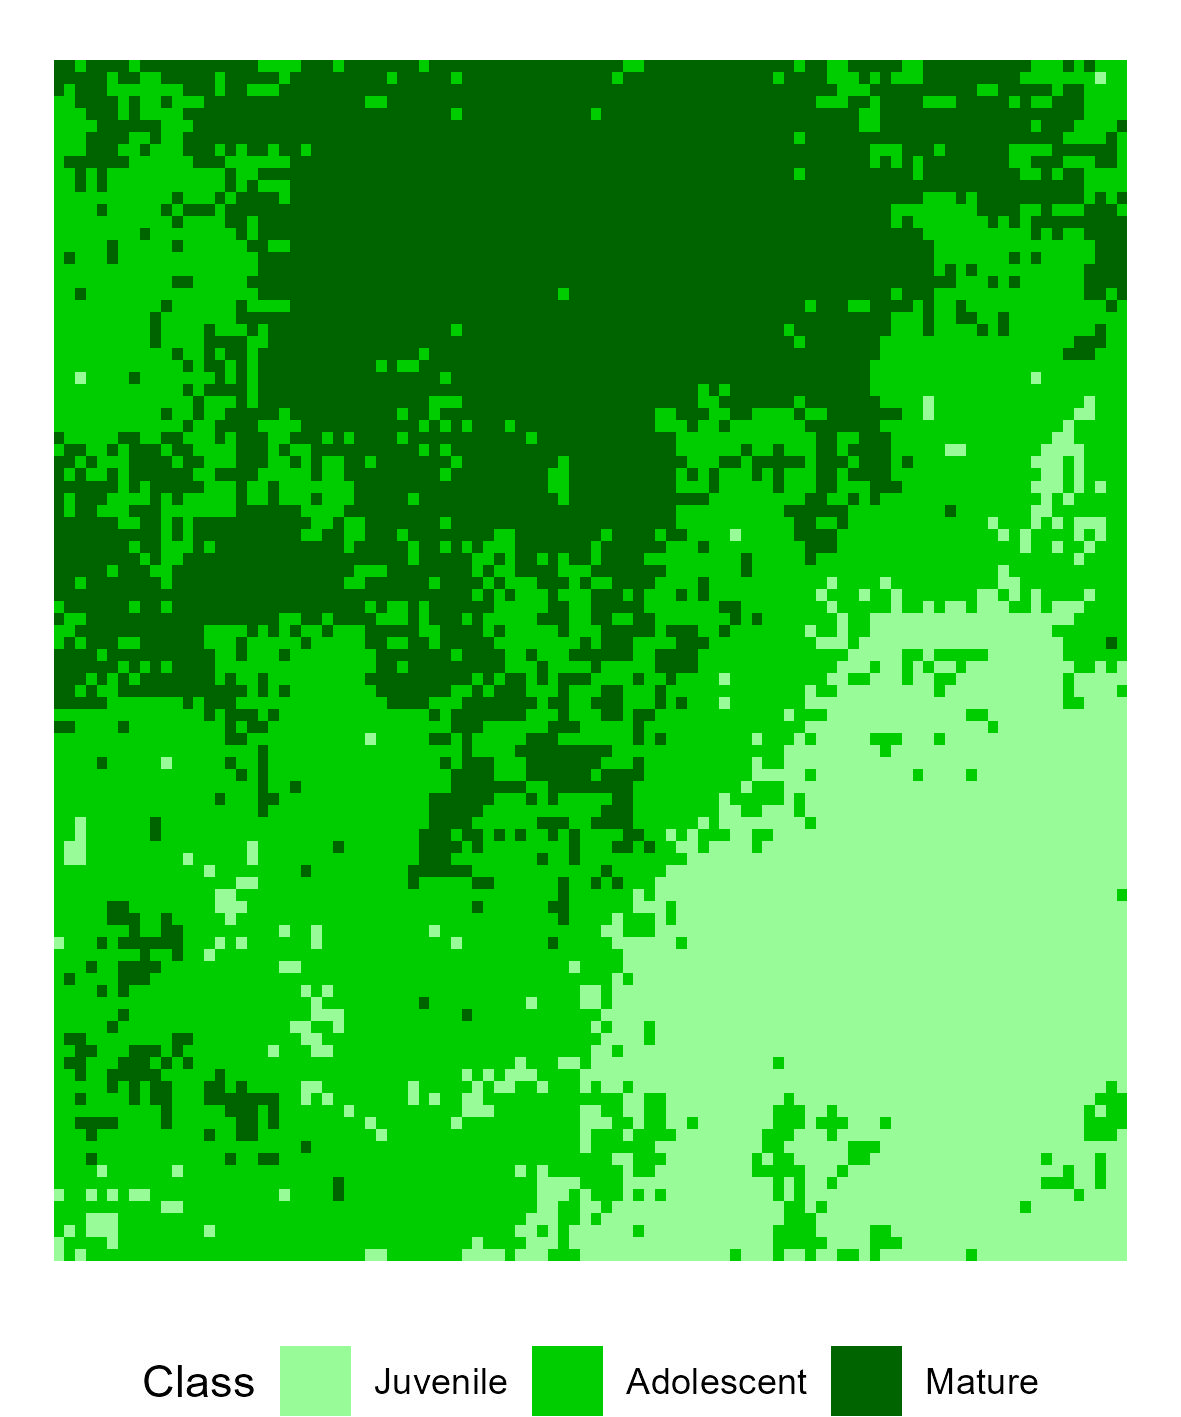
\includegraphics[width=0.4\linewidth]{figures/wildland/large_land_autocorr_0.5_distrib_1}
    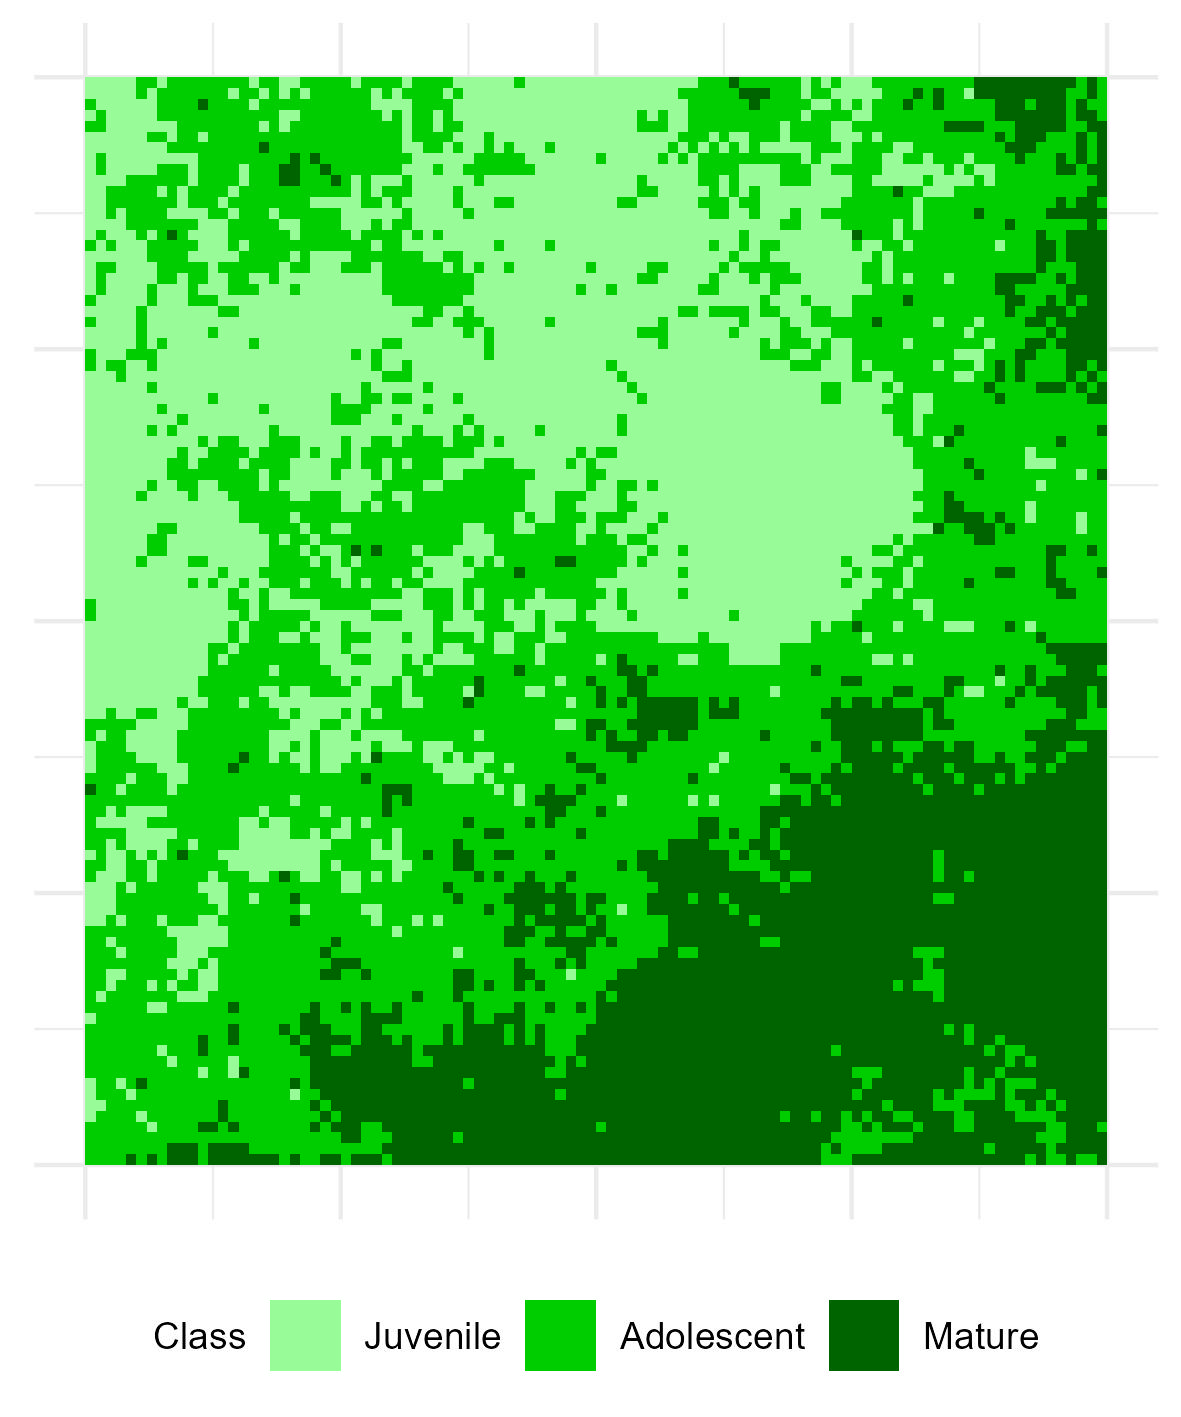
\includegraphics[width=0.4\linewidth]{figures/wildland/large_land_autocorr_0.5_distrib_4}\\
    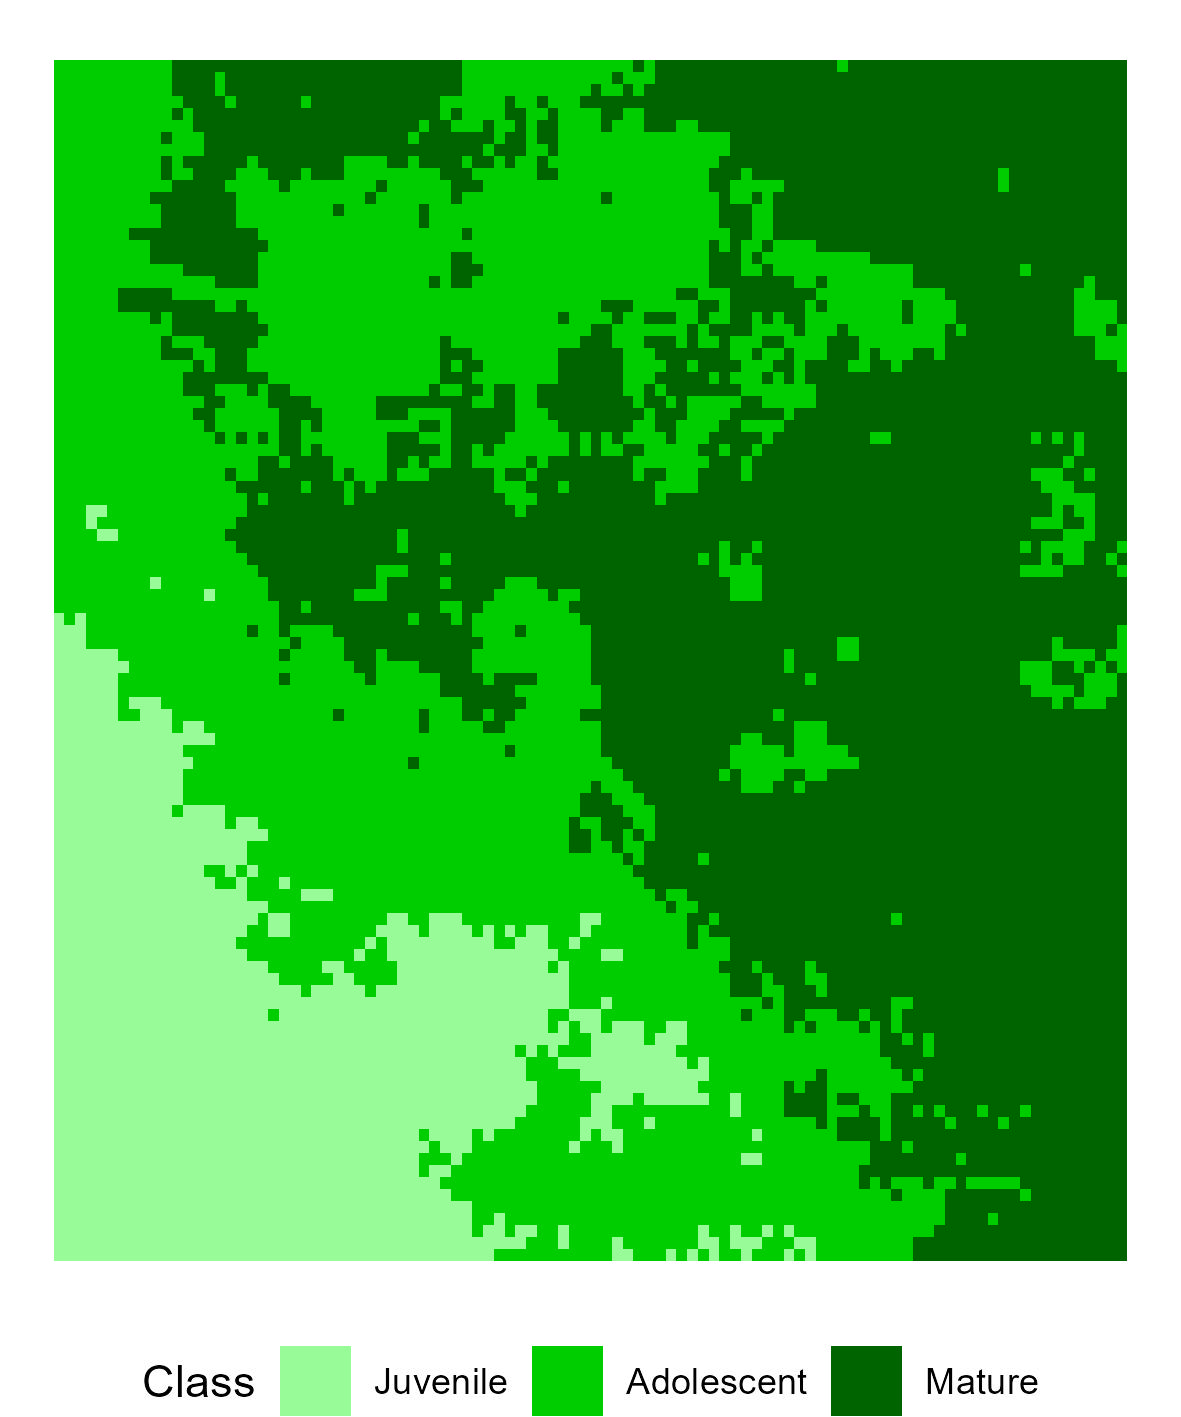
\includegraphics[width=0.4\linewidth]{figures/wildland/large_land_autocorr_0.9_distrib_1}
    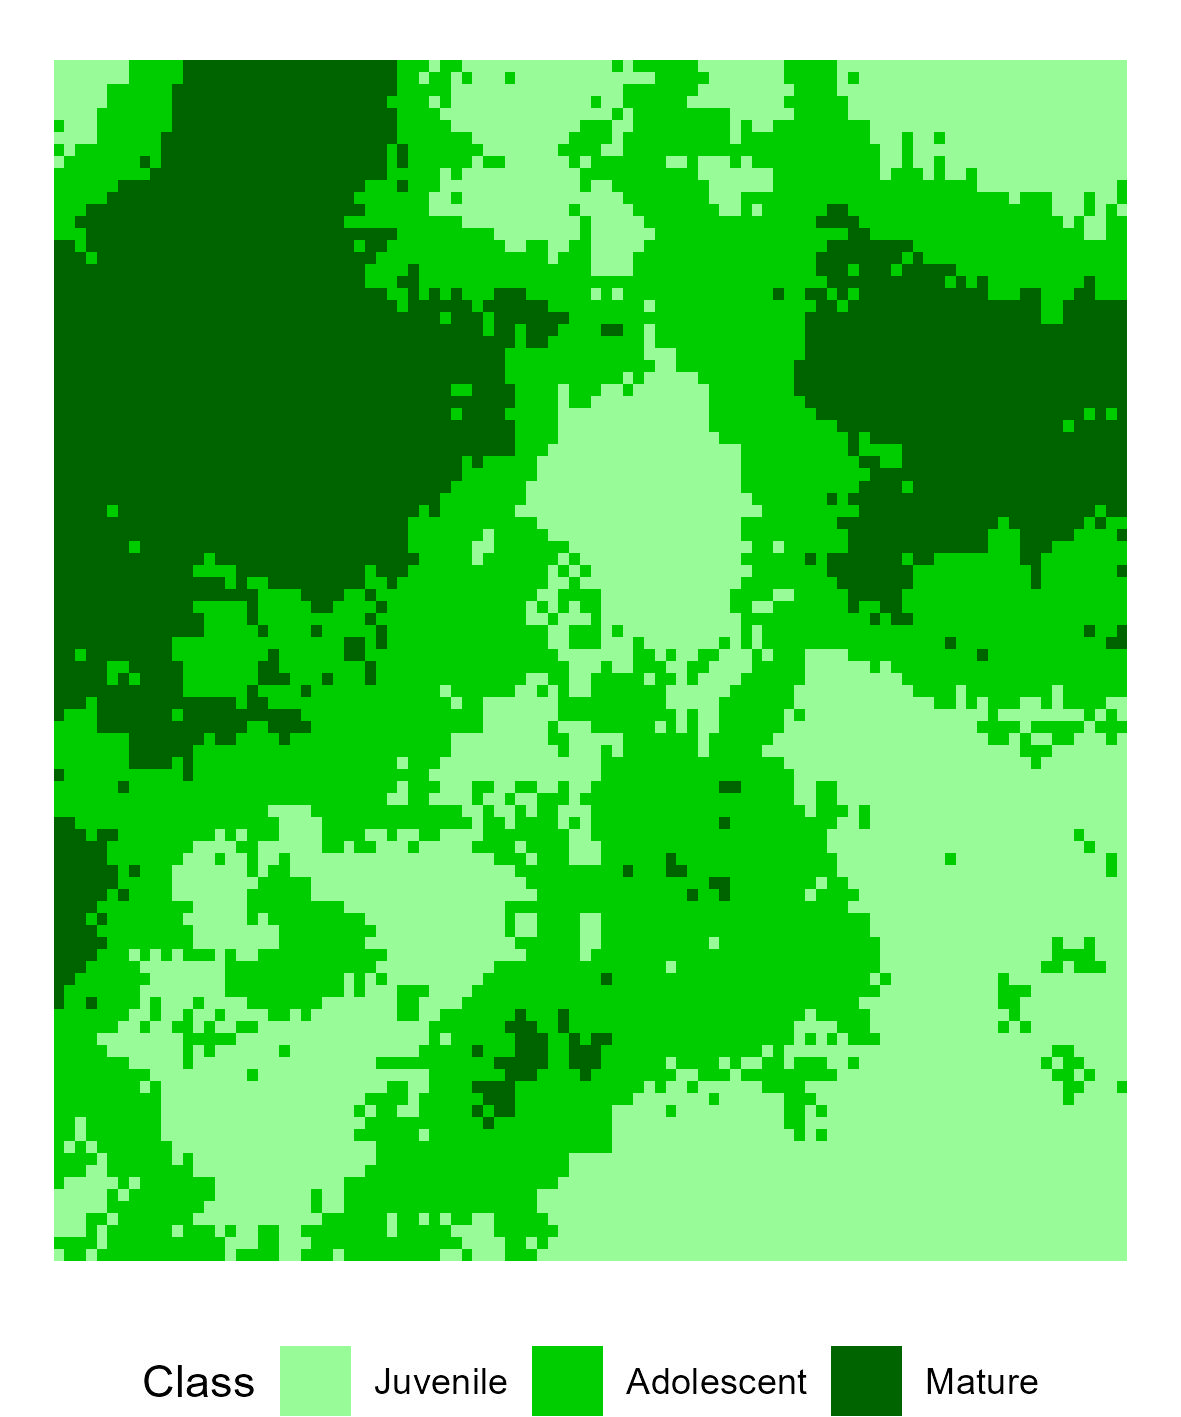
\includegraphics[width=0.4\linewidth]{figures/wildland/large_land_autocorr_0.9_distrib_4}\\
    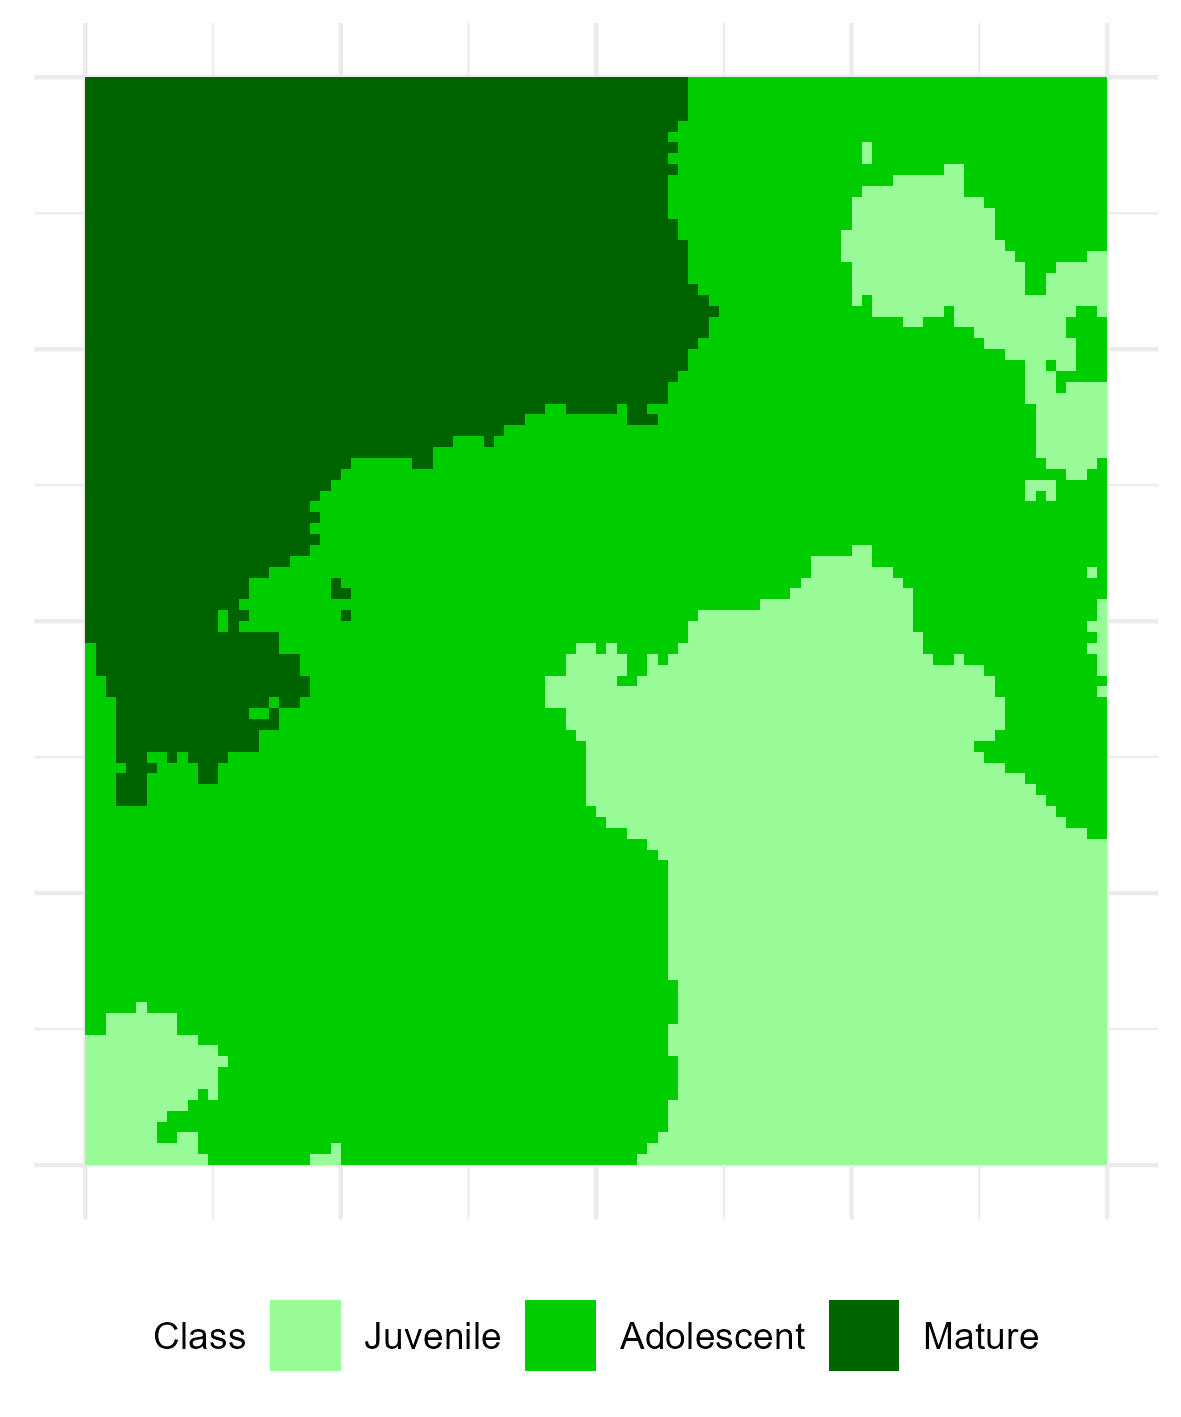
\includegraphics[width=0.4\linewidth]{figures/wildland/large_land_autocorr_1.8_distrib_1}
    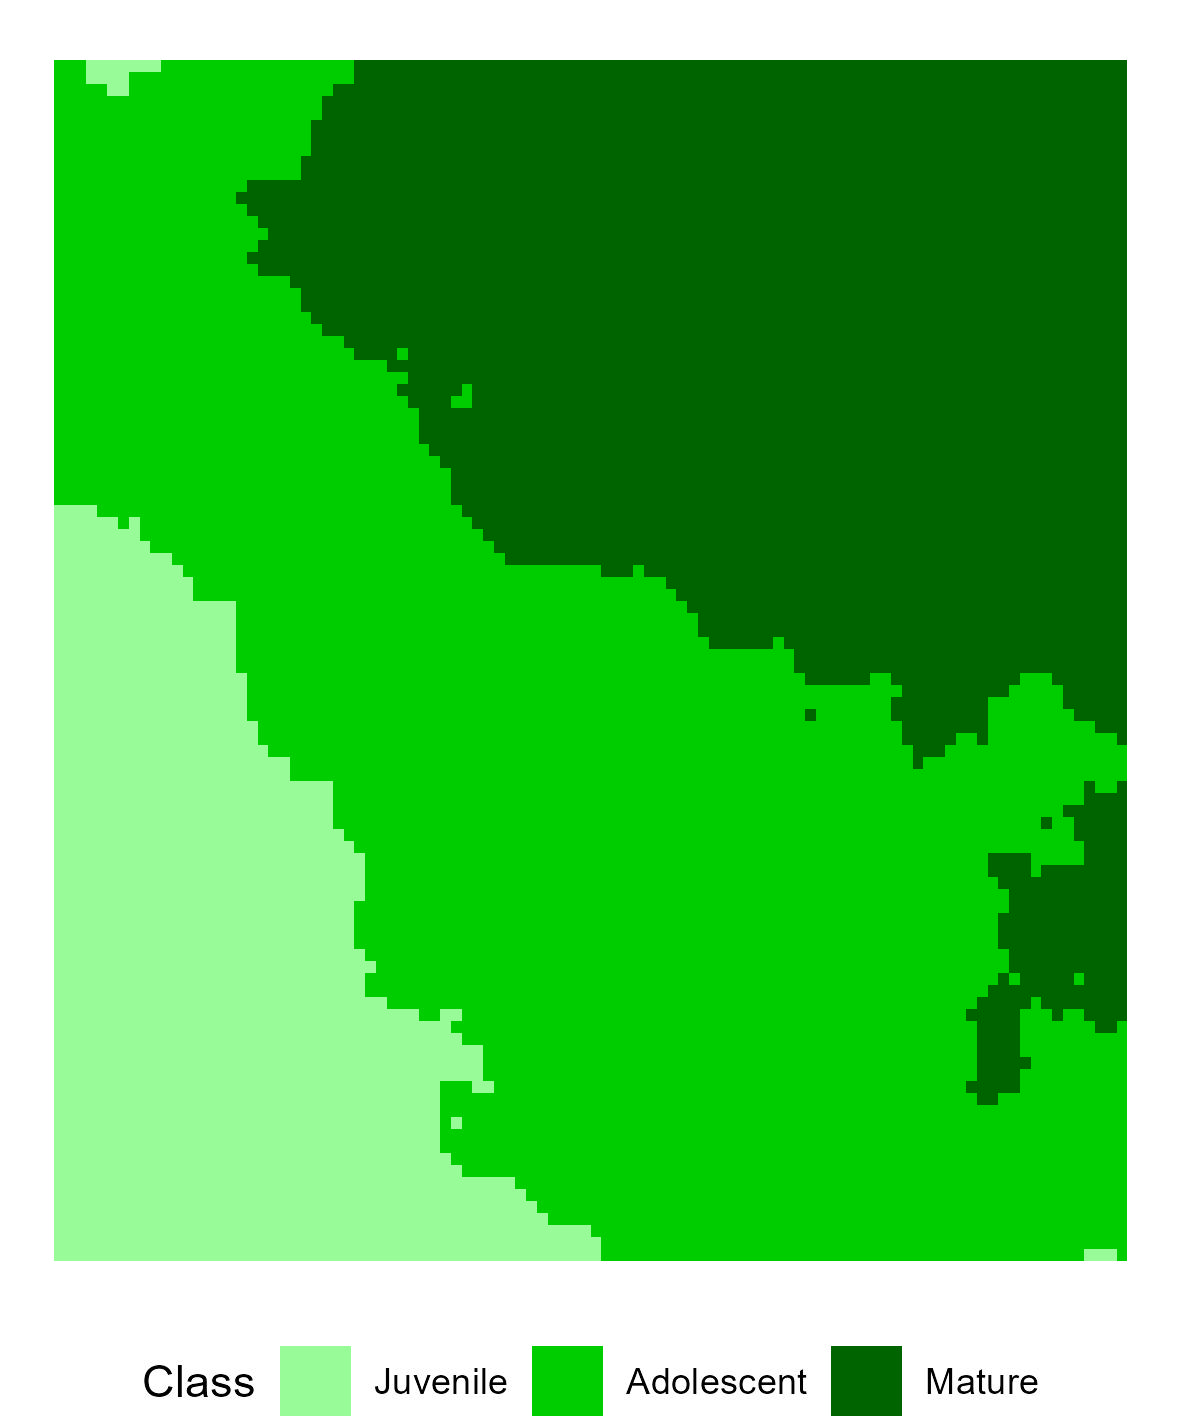
\includegraphics[width=0.4\linewidth]{figures/wildland/large_land_autocorr_1.8_distrib_4}
    \caption{Examples of large scale landscapes with uniform distribution (left) and skewed towards \textit{adolescent} (right)and low, middle and large spatial autocorrelation}
    \label{fig:ex_nlm}
\end{figure}
\clearpage





\subsection{Landscape indicators}
\label{sec:appendix_wildland__indicators}

\paragraph{Area}
We use the number of vertices (nodes) for both graphs:

\begin{equation}
Area(\mathcal{G}_t) = \mathrm{card}(V_{\mathcal{G}_t}) \text{ with } \mathcal{G}_t\in\{\mathcal{B}_t,\mathcal{F}_t\}
\label{eq:area}
\end{equation}

%\paragraph{Number of components}

%\begin{equation}
%    \# components_i = card(\text{Maximal connected subgraphs of } G_i \text{ for } i \in \{B,F\})
%    \label{eq:components}
%\end{equation}

\paragraph{Simpson diversity index:}
Let $p_i$ be the proportion of landscape $A_t$ in a given succesional stage\footnote{Let $Juv = \{a_{ijt} \text{ such that } a_{ijt}=0\}$, then $p_{Juv} = \frac{\mathrm{card}(Juv)}{n^2}$}, the Simpson diversity index is : 

\begin{equation}
SIDI = 1 - \sum_{i \in \{Juv, Ado, Mat\}} p_i^2
    \label{eq:simpson}
\end{equation}


\paragraph{Landscape shape index:}
following \cite{McGarigal_1995}, the adapted LSI index from \cite{patton_diversity_1975} in a raster landscape is:
\begin{equation}
    LSI = \frac{0.25\times perimeter(G)}{n}
    \label{eq:LSI}
\end{equation}
Where $perimeter(G)$ is the perimeter of the cells comprised in the graph as vertices.

\paragraph{Successional Stage Heterogeneity Index:} let $d_{ij}$ be a binary variable such that $d_{ij}=1$ if patch $i$ and $j$ share the same successional stage. Define $\mathcal{J}$ as the set of neighbors in 4 directions (north, south, east, west) of cell $i$\footnote{The set $\mathcal{J}_i$ varies with cell $i$ to account for edge effects}.
The successional stage heterogeneity index is : 
\begin{equation}
    SSHI = 1 - \frac{1}{N}\sum_{i=1}^N\left( \frac{\sum_{j \in \mathcal{J}_i} d_{ij}}{\mathrm{card}(\mathcal{J}_i)}\right)
\end{equation}
\label{eq:lth_index}


\clearpage

\subsection{Treatment centrality indicators}
\label{sec:treatment_centrality_appendix}
\textbf{Betweennness centrality:} take a graph $\mathcal{G}(V,E)$ and let $\sigma_{st}$ be the total number of shortest paths from node $s$ to $t$ and $\sigma_{st}(v)$ be the number of those paths that pass through $v$, for $\{s,t,v\} \subset V$, betweenness centrality is given by :
\begin{equation}
g(v) = \sum_{s\neq v \neq t} \frac{\sigma_{st}(v)}{\sigma_{st}}
\end{equation}

\textbf{Eigencentrality:} let $\mathbf{A}\in \mathcal{M}_{n,n}$ be the adjacency matrix of graph and $a_{i,j}=1$ if vertices $i$ and $j$ are connected. Let $\lambda \in \mathbb{R}^{n^2}$, and a vector $\mathbf{x} \in \mathbb{R}^{n^2}$, such that $\lambda \mathbf{x} = \mathbf{Ax}$ e.g $\lambda$ is the eigenvalue of matrix $\mathbf{A}$. Using this eigenvalue, \textit{centrality scores} are computed as :
\begin{equation}
\text{score}(x_i)= \frac{1}{\lambda}\sum_{j \in V_{\mathcal{G}_t}} a_{i,j}x_j
\end{equation}

\textbf{Subgraph centrality:} In a graph, a \textit{walk} is a sequence of adjacent vertices in a graph. A \textit{closed walk} is a walk with identical beginning and ending vertices, and can be of order $k$ e.g. of length equal to $k$ edges. The number of \textit{closed walks of order $k$} is found using the adjacency matrix $\mathbf{A}$ of a graph. Let $\mu_k(i)$ be the number of closed walks of order $k$ starting at $i$ : 

$$
\mu_k(i) = (\mathbf{A}^k)_{i,i}
$$

Subgraph centrality is defined as : 
\begin{equation}
SC(i) = \sum_{k=0}^\infty \frac{\mu_k(i)}{k!}
\end{equation}

\cite{estrada_subgraph_2005}, who define this notion, show that it can be reformulated with the eigenvalues and eigenvectors of the adjacency matrix $\mathbf{A}$ of a graph $\mathcal{G}(V,E)$ of order $n$. Let $v_{1},...,v_{n}$ be a an orthornomal basis of $\mathbb{R}^N$ composed of eigevenctors of $\mathbf{A}$ associated to the eigenvalues $\lambda_1, ..., \lambda_N$, and let $v^i_j$ be the \textit{i}-the component of $v_j$, then subgraph centrality can be expressed, for all $v in V$:

\begin{equation}
SC(i) = \sum_{j=1}^N(v^i_j)^2 e^{\lambda_j}
\end{equation}

\clearpage

\subsection{Additional figures}



\begin{figure}[H]
    \centering
 %   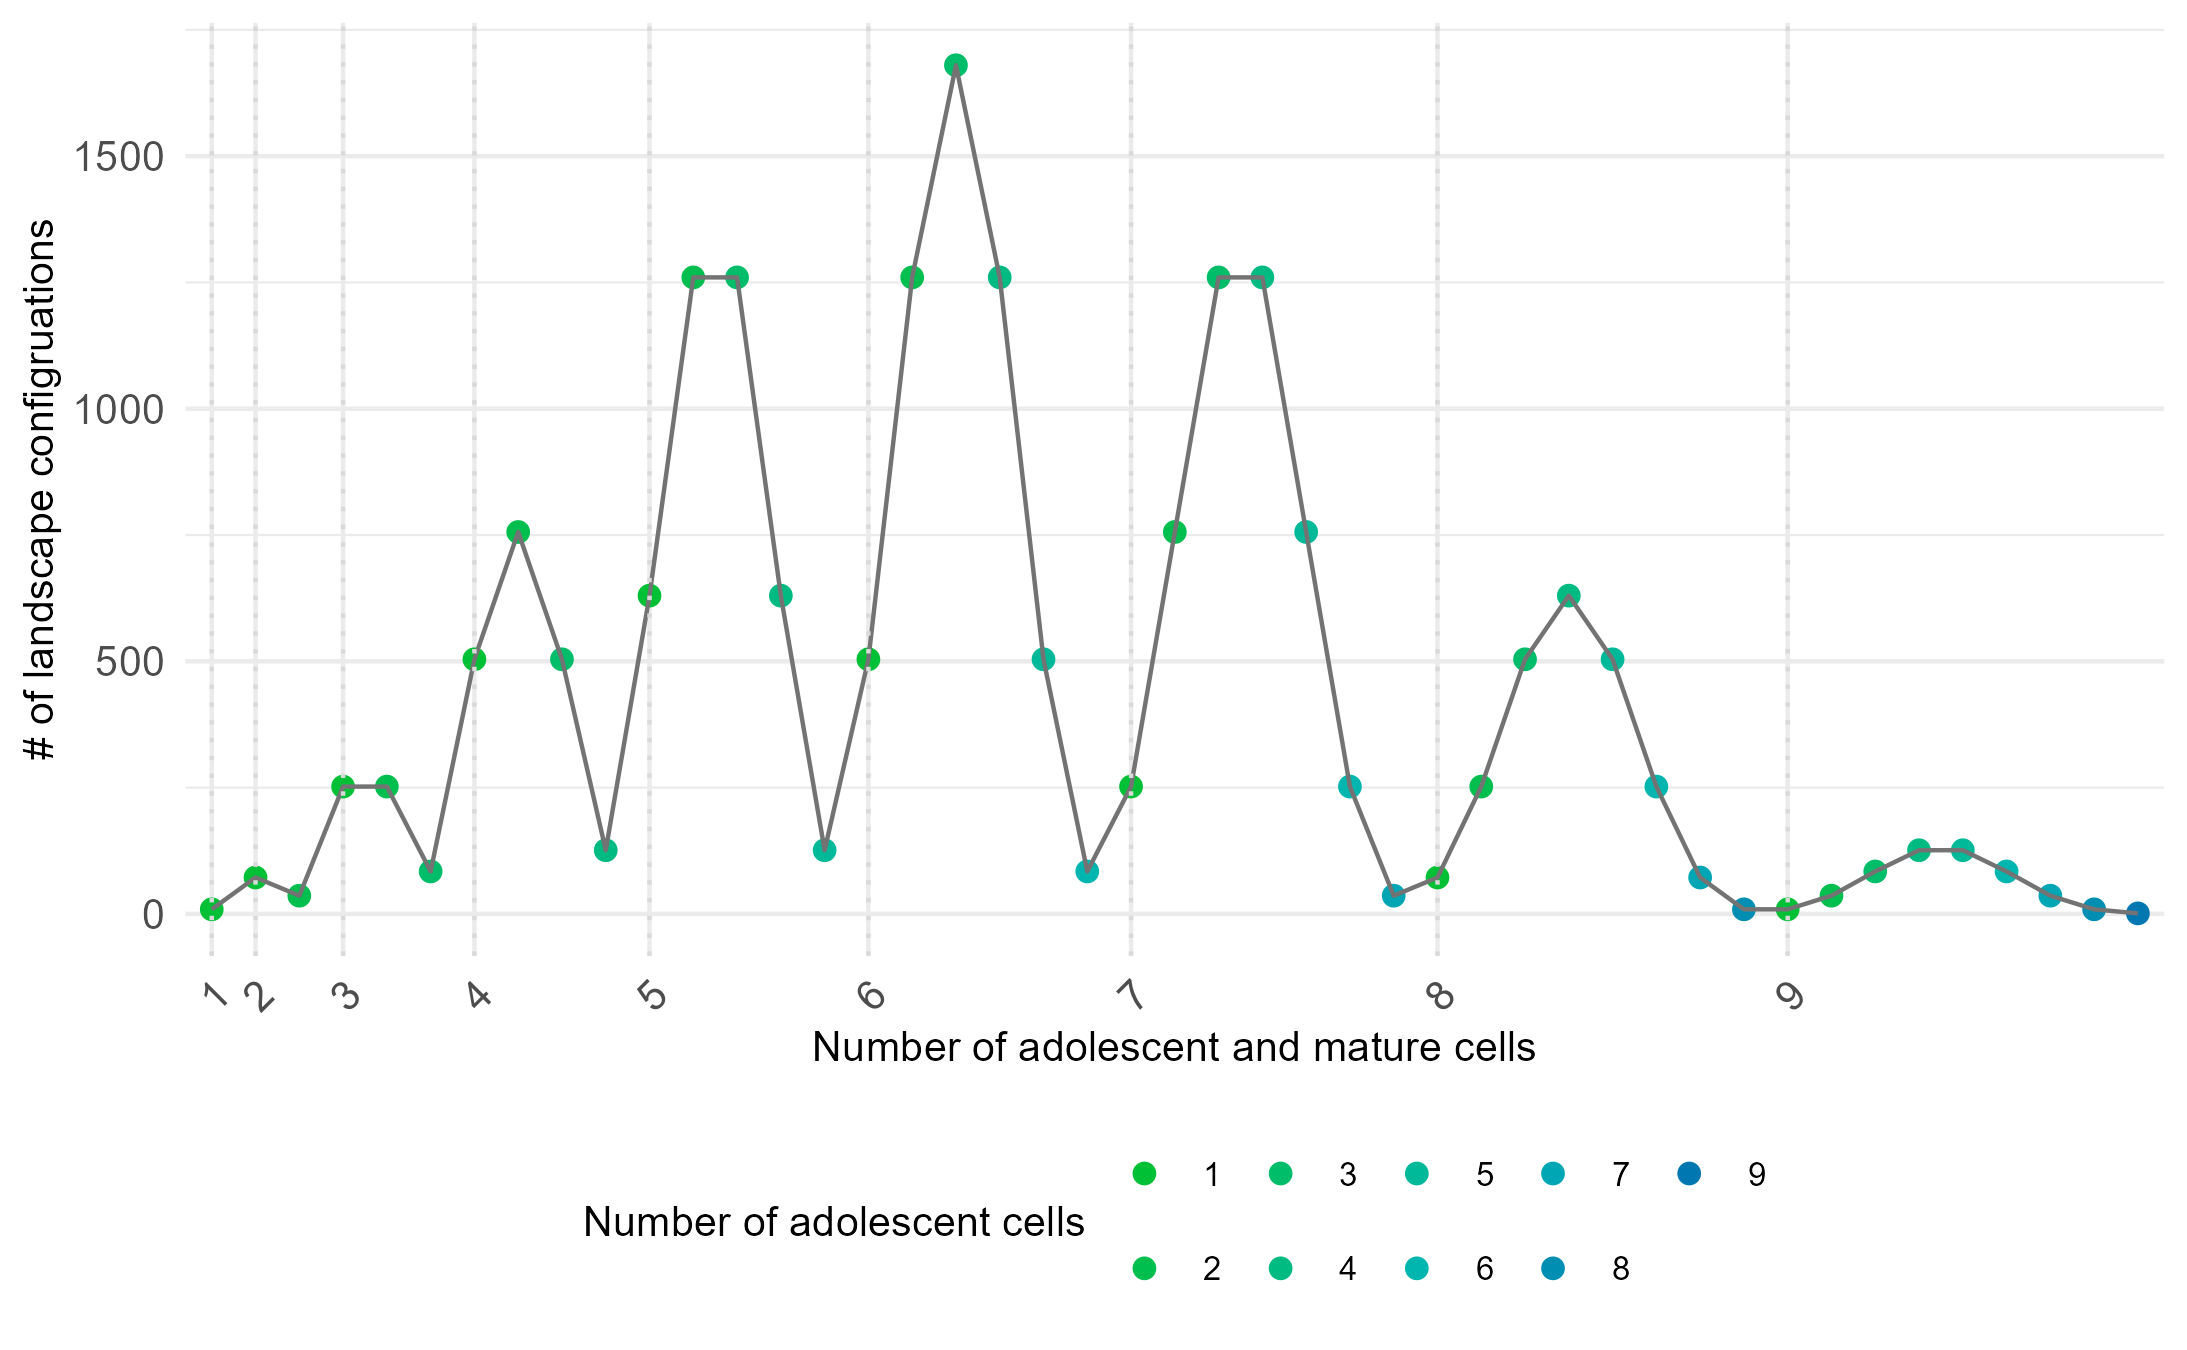
\includegraphics[width = 0.8\textwidth]{figures/wildland/distribution_cases_3.png}\\
    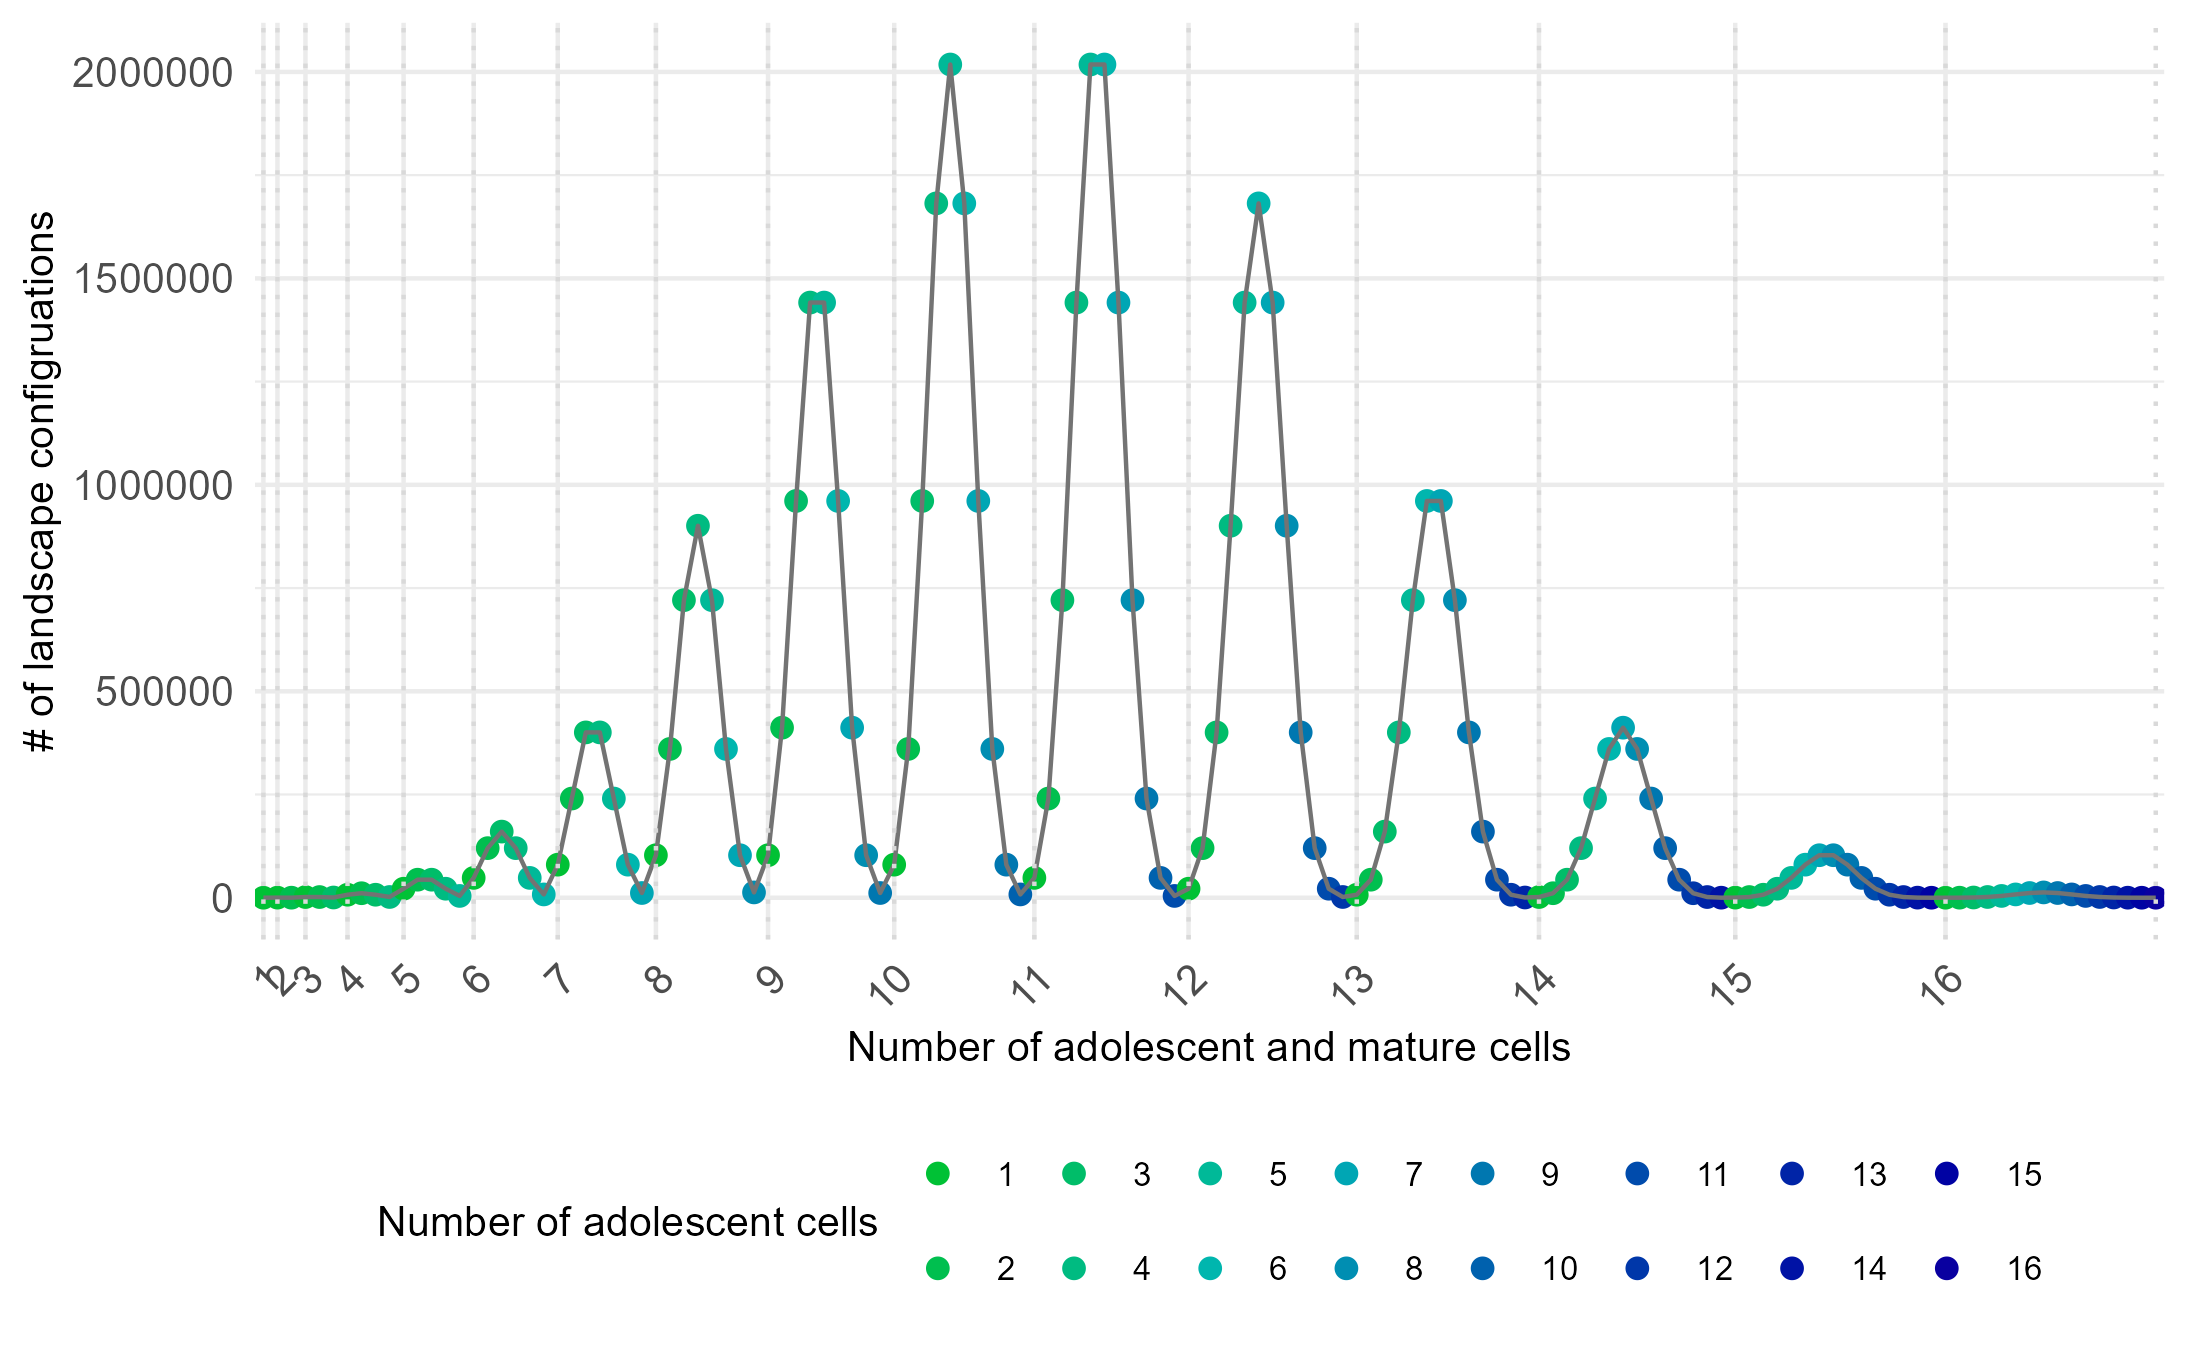
\includegraphics[width = 0.8\textwidth]{figures/wildland/distribution_cases_4.png}
    \caption{Distribution of number of landscapes depending on number of \textit{juvenile, adolescent}, and \textit{mature} cells for sizes $\in \{3,4\}$}
    \subcaption*{Each number on the $x$ axis represents the cumulated number of \textit{adolescent} and \textit{mature} cells among the landscape. Between each number on the $x$-axis is the number of \textit{adolescent} cells among the number of cumulated \textit{adolescent} and \textit{mature cells}. For example, the highest point of the distribution, between $11$ and $12$, represent the number of possible combinations of landscapes with a cumulated number of \textit{adolescent} and \textit{mature} cells of 11, with 5 and 6 \textit{adolescent cells} e.g. 6 and 5 (respectively) \textit{mature cells}}
    \label{fig:appendix_distribution}
\end{figure}

\begin{figure}[H]
    \centering
    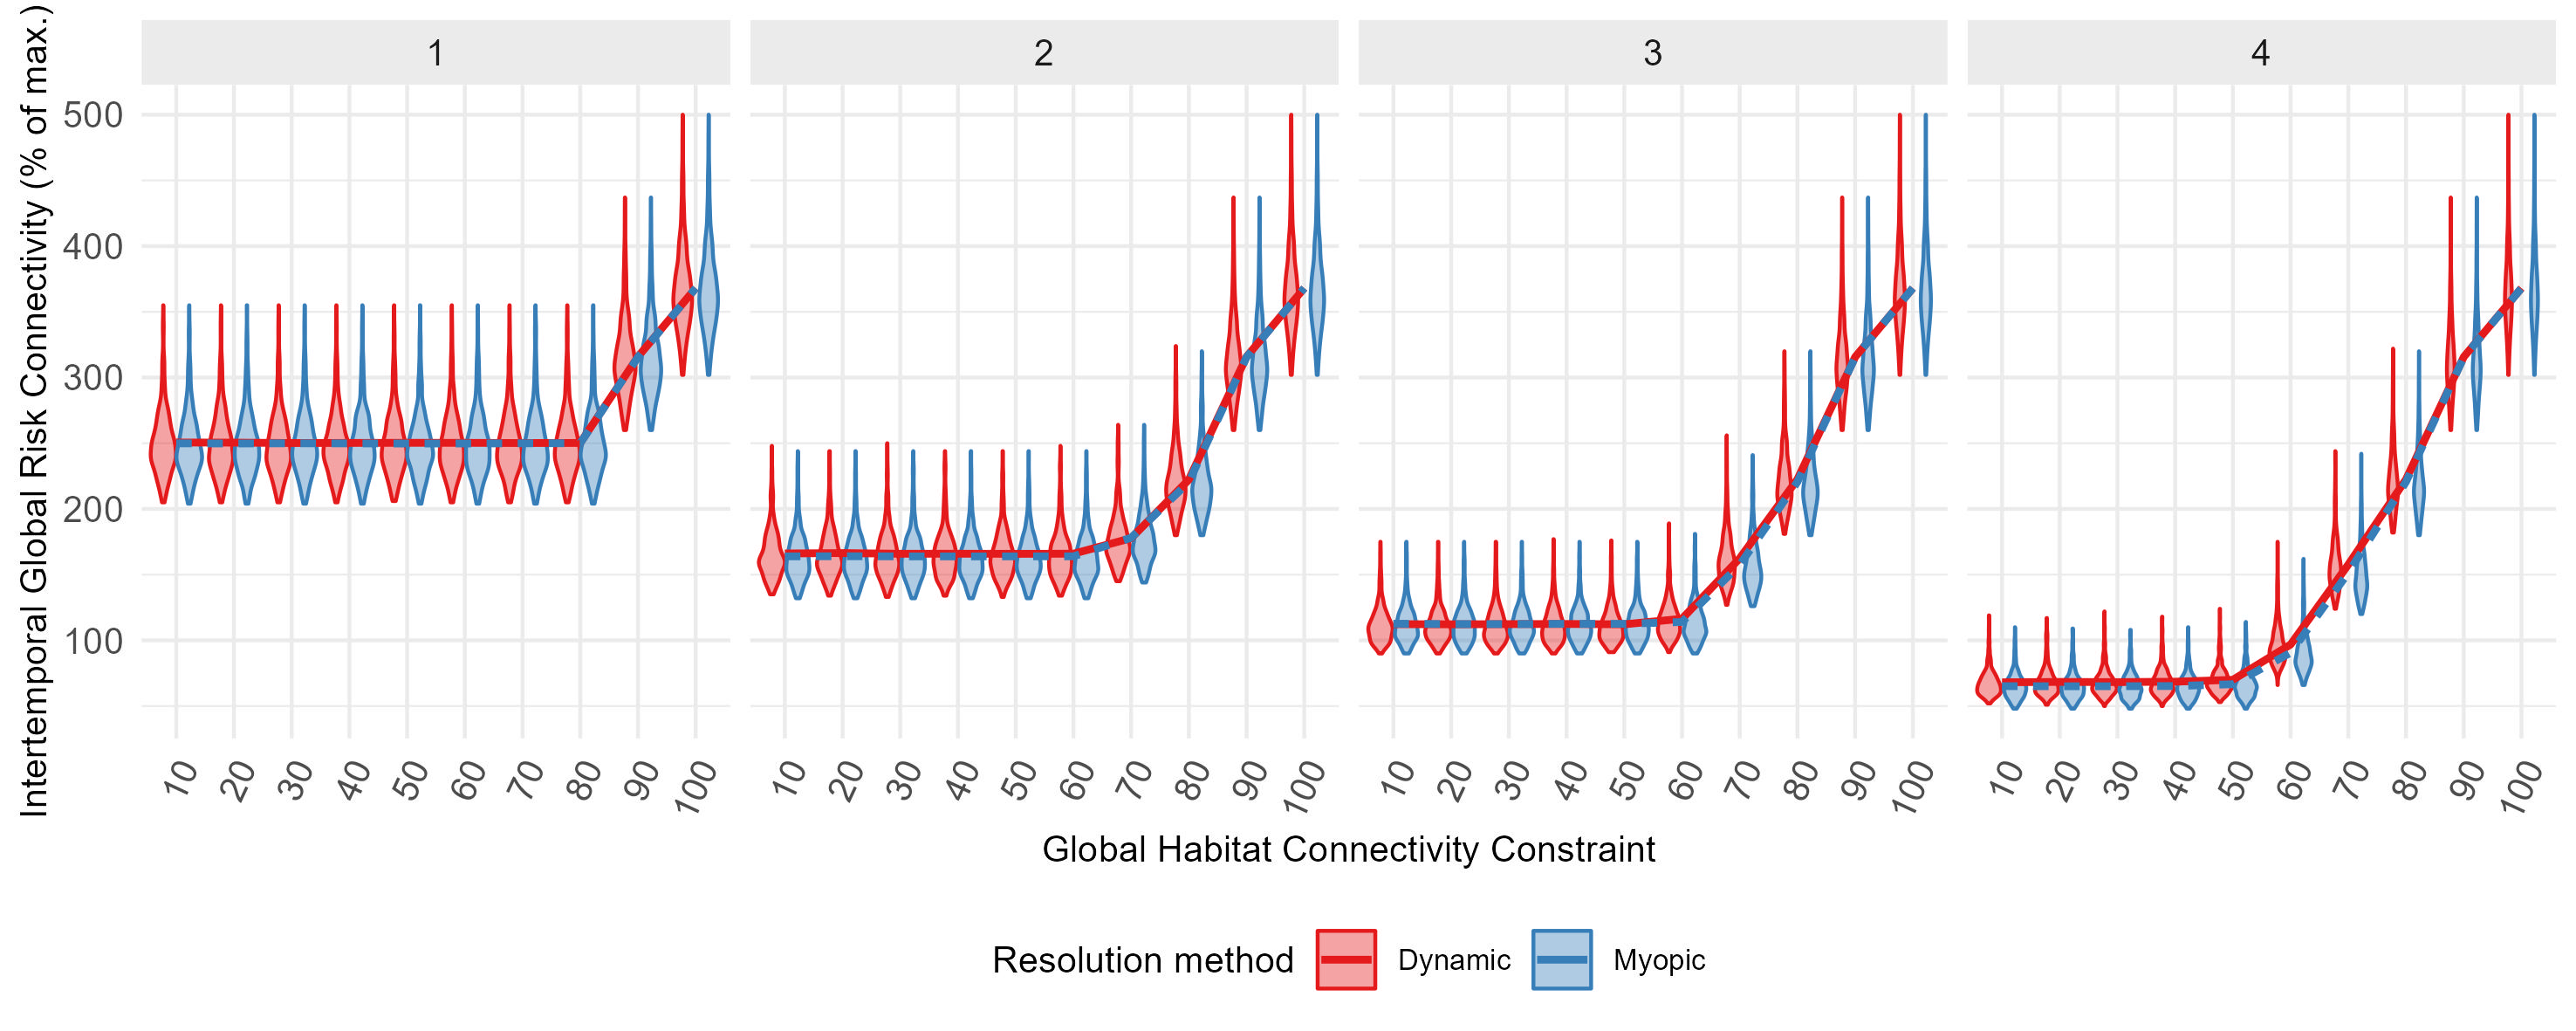
\includegraphics[width=\textwidth]{figures/wildland/dynamic_v_myopic_fpp.jpg}
    \caption{Production possibility frontiers between global risk connectivity and global habitat connectivity constraints across budget constraint levels for the sample of representative landscapes of size $n=4$ between repeated myopic and dynamic optimization procedures for $T=5$}
    \label{fig:appendix_fpp_dyn_myopic}
\end{figure}
\clearpage

% Table created by stargazer v.5.2.3 by Marek Hlavac, Social Policy Institute. E-mail: marek.hlavac at gmail.com
% Date and time: jeu., sept. 05, 2024 - 17:16:49

\begin{figure}[h]
	\centering
	\begin{subfigure}[b]{\textwidth}
		\centering
	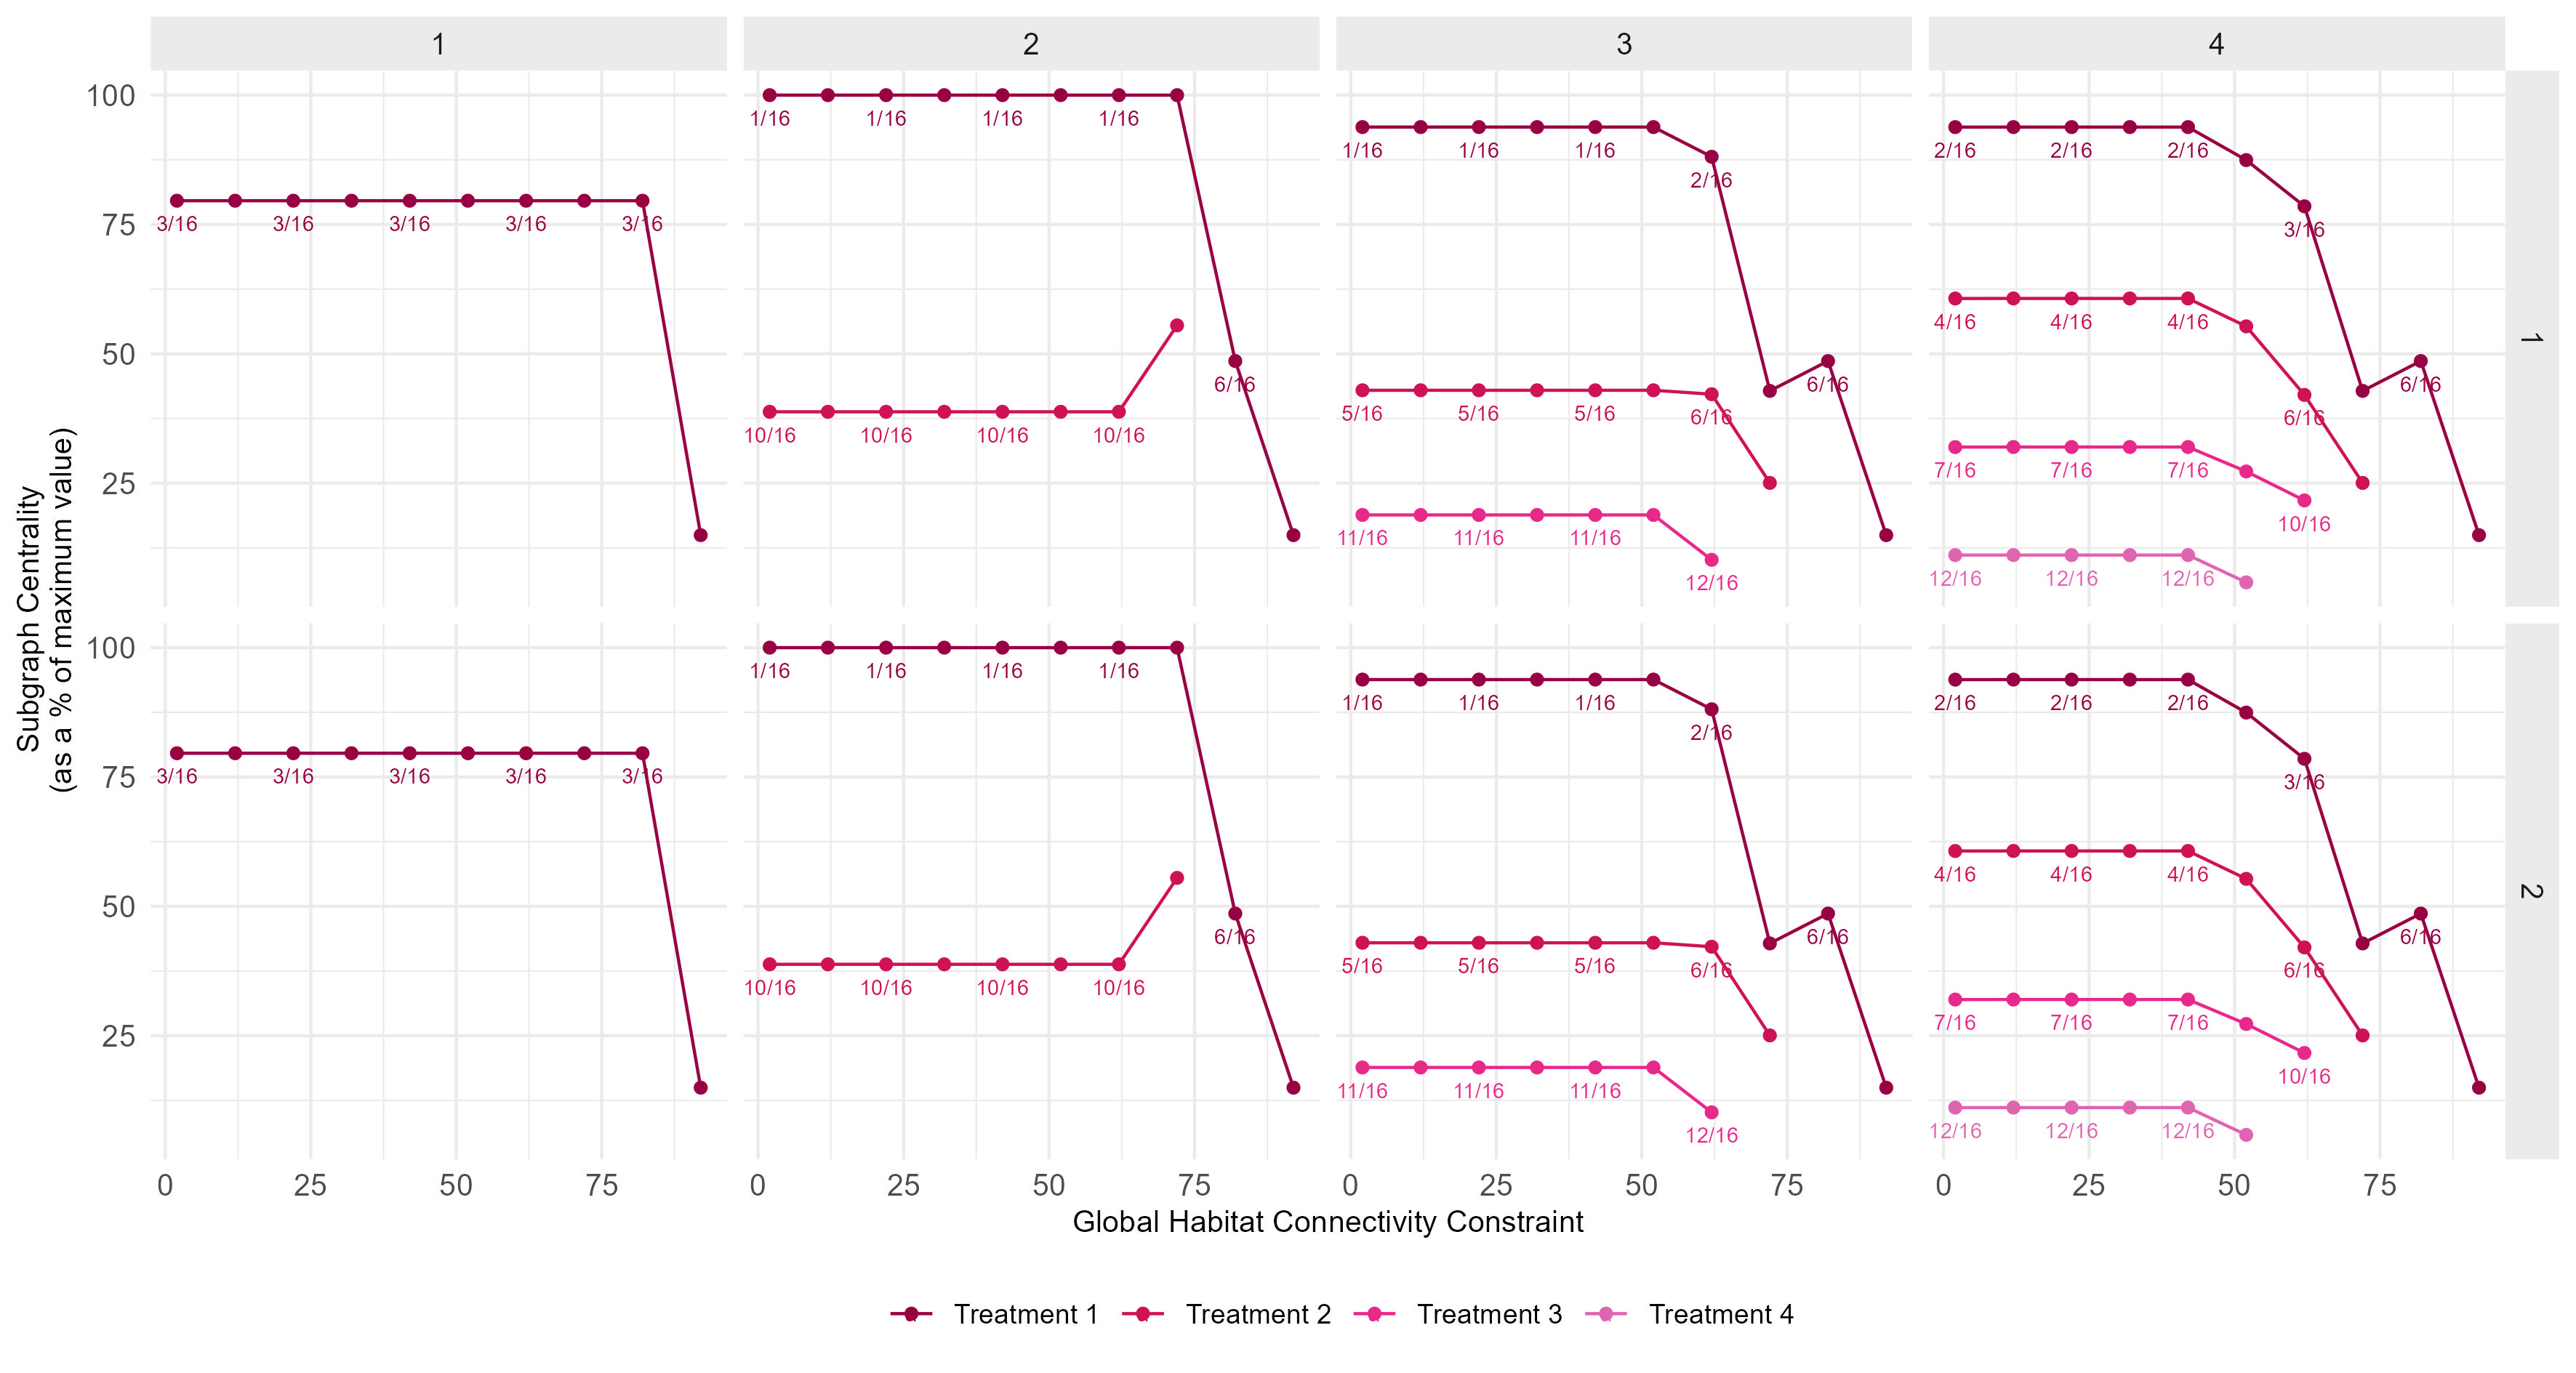
\includegraphics[width = .8\textwidth]{figures/wildland/subgraph_treatment.jpg}
	\caption{Subgraph centrality of treated vertices (average value and rank)}
	\label{fig:subgraph}
	\end{subfigure}
	
	\begin{subfigure}[b]{\textwidth}
	\centering
	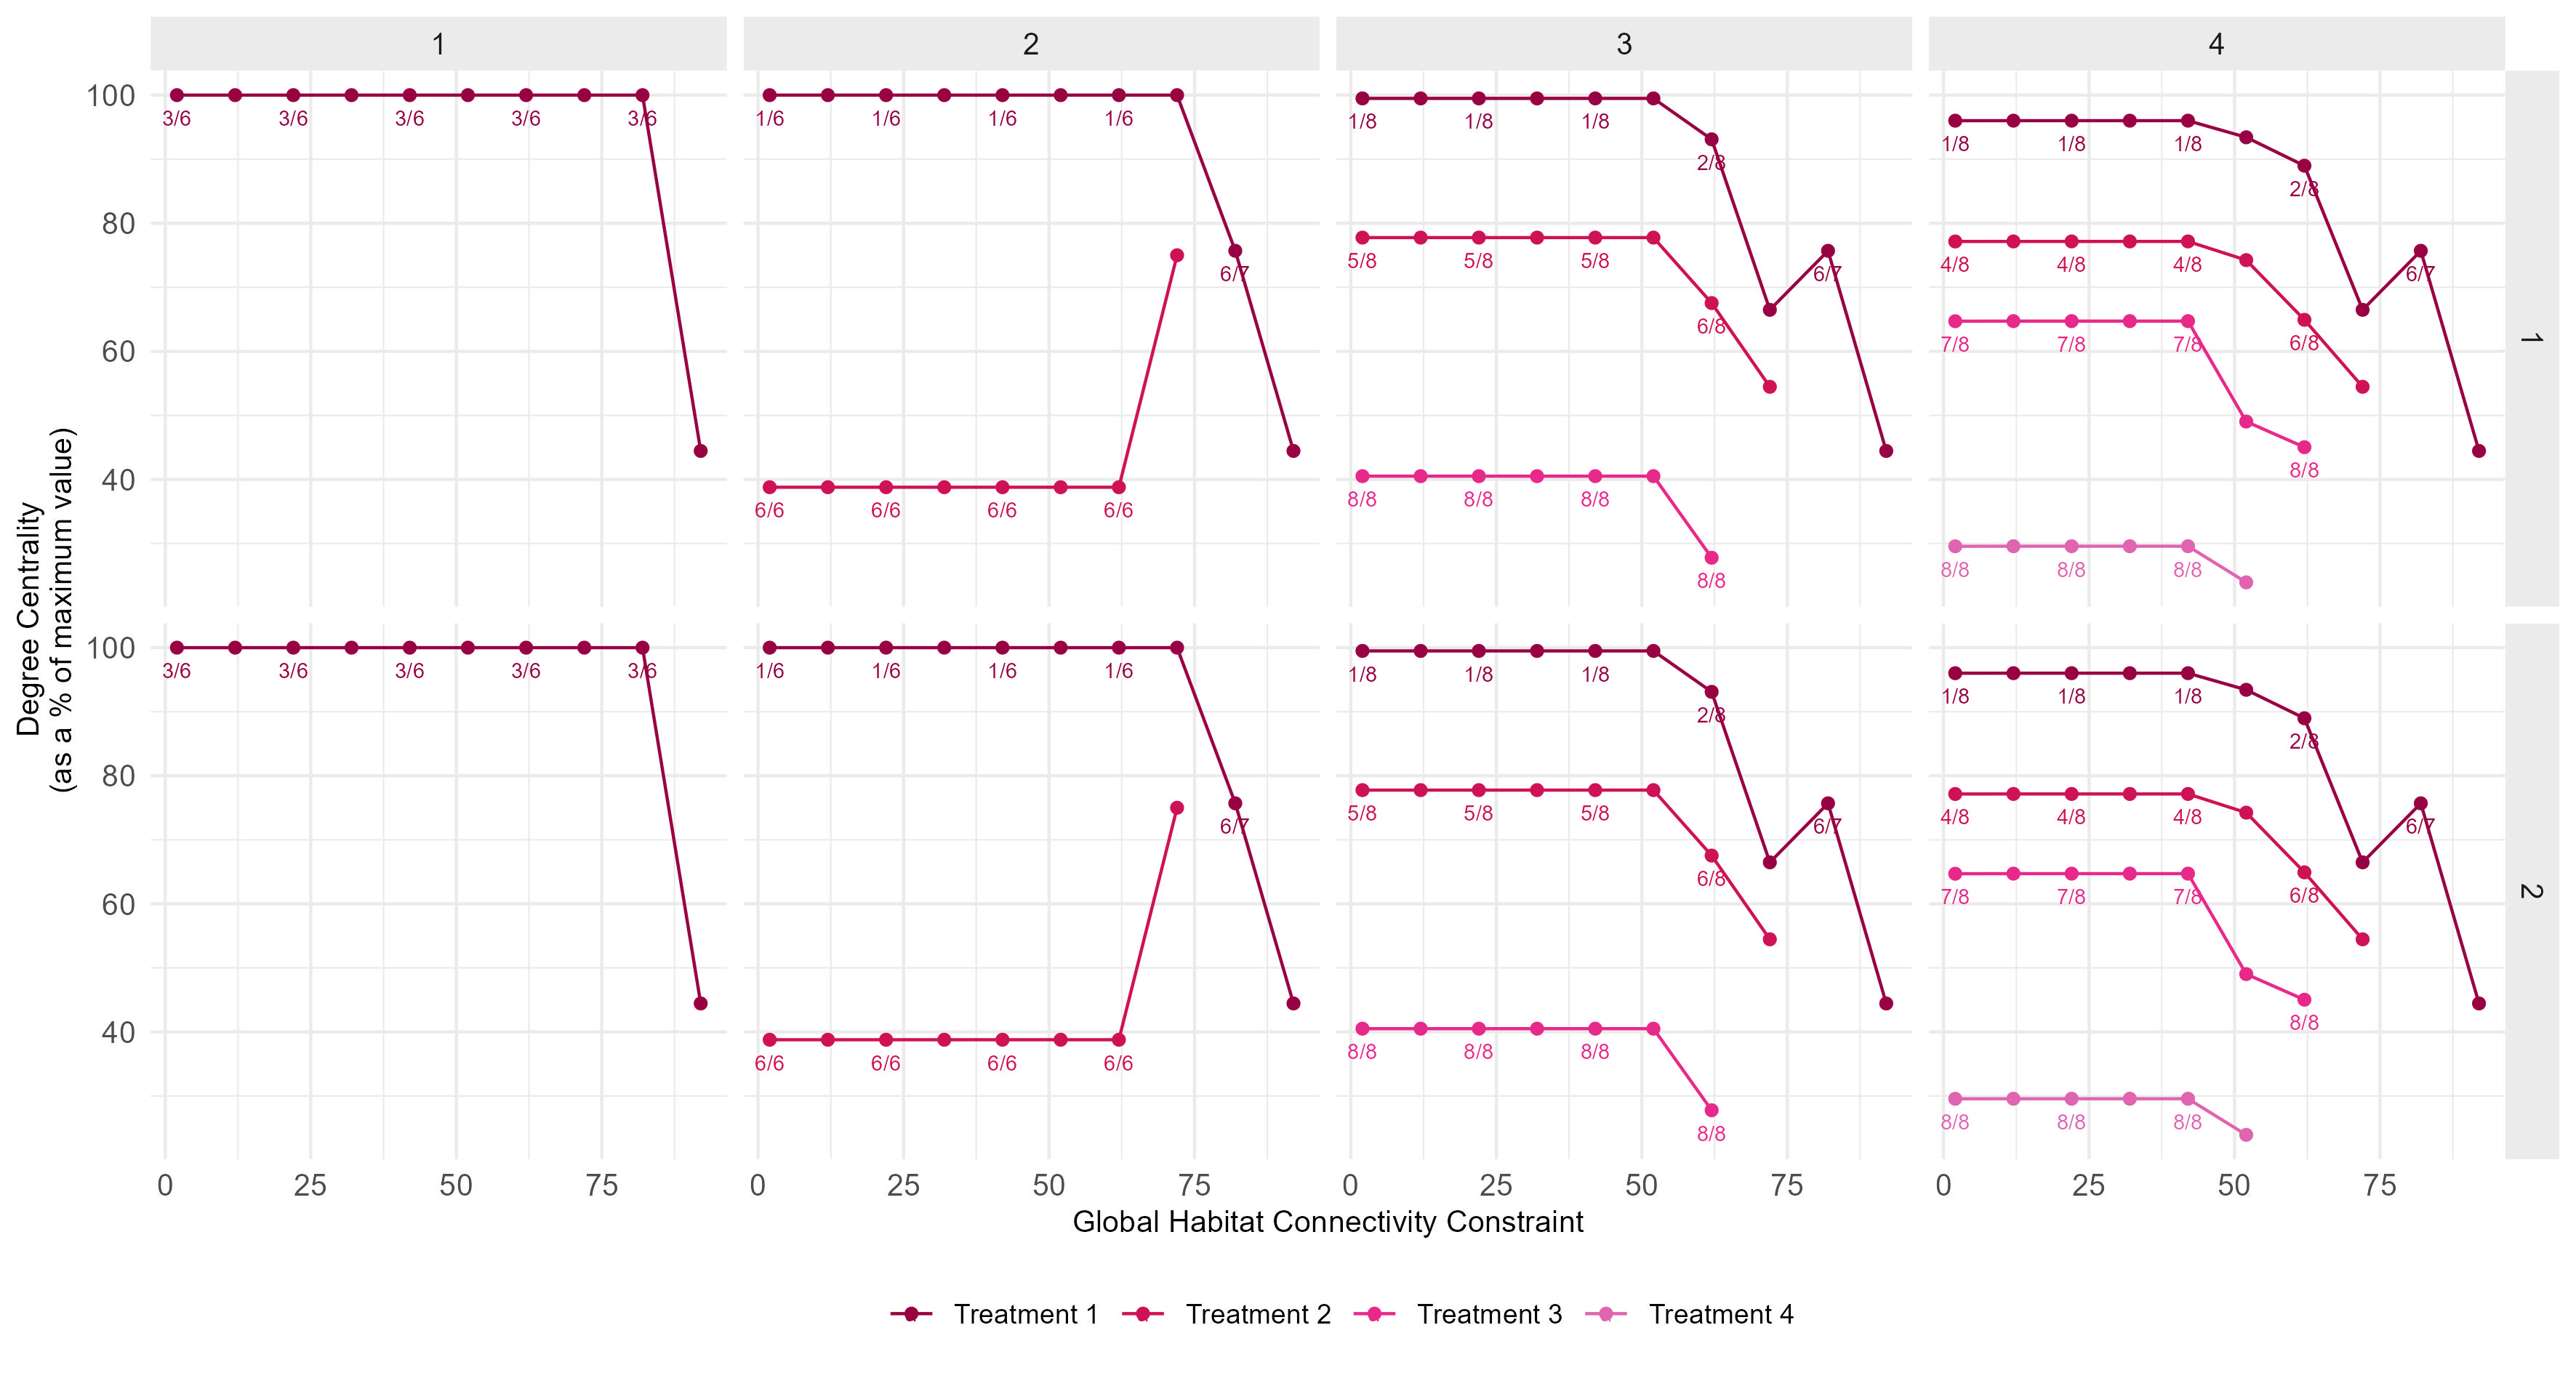
\includegraphics[width = .8\textwidth]{figures/wildland/degree_treatment.jpg}
	\caption{Degree centrality of treated vertices (average value and rank)}
	\label{fig:degree}
	\end{subfigure}

	\begin{subfigure}[b]{\textwidth}
	\centering
	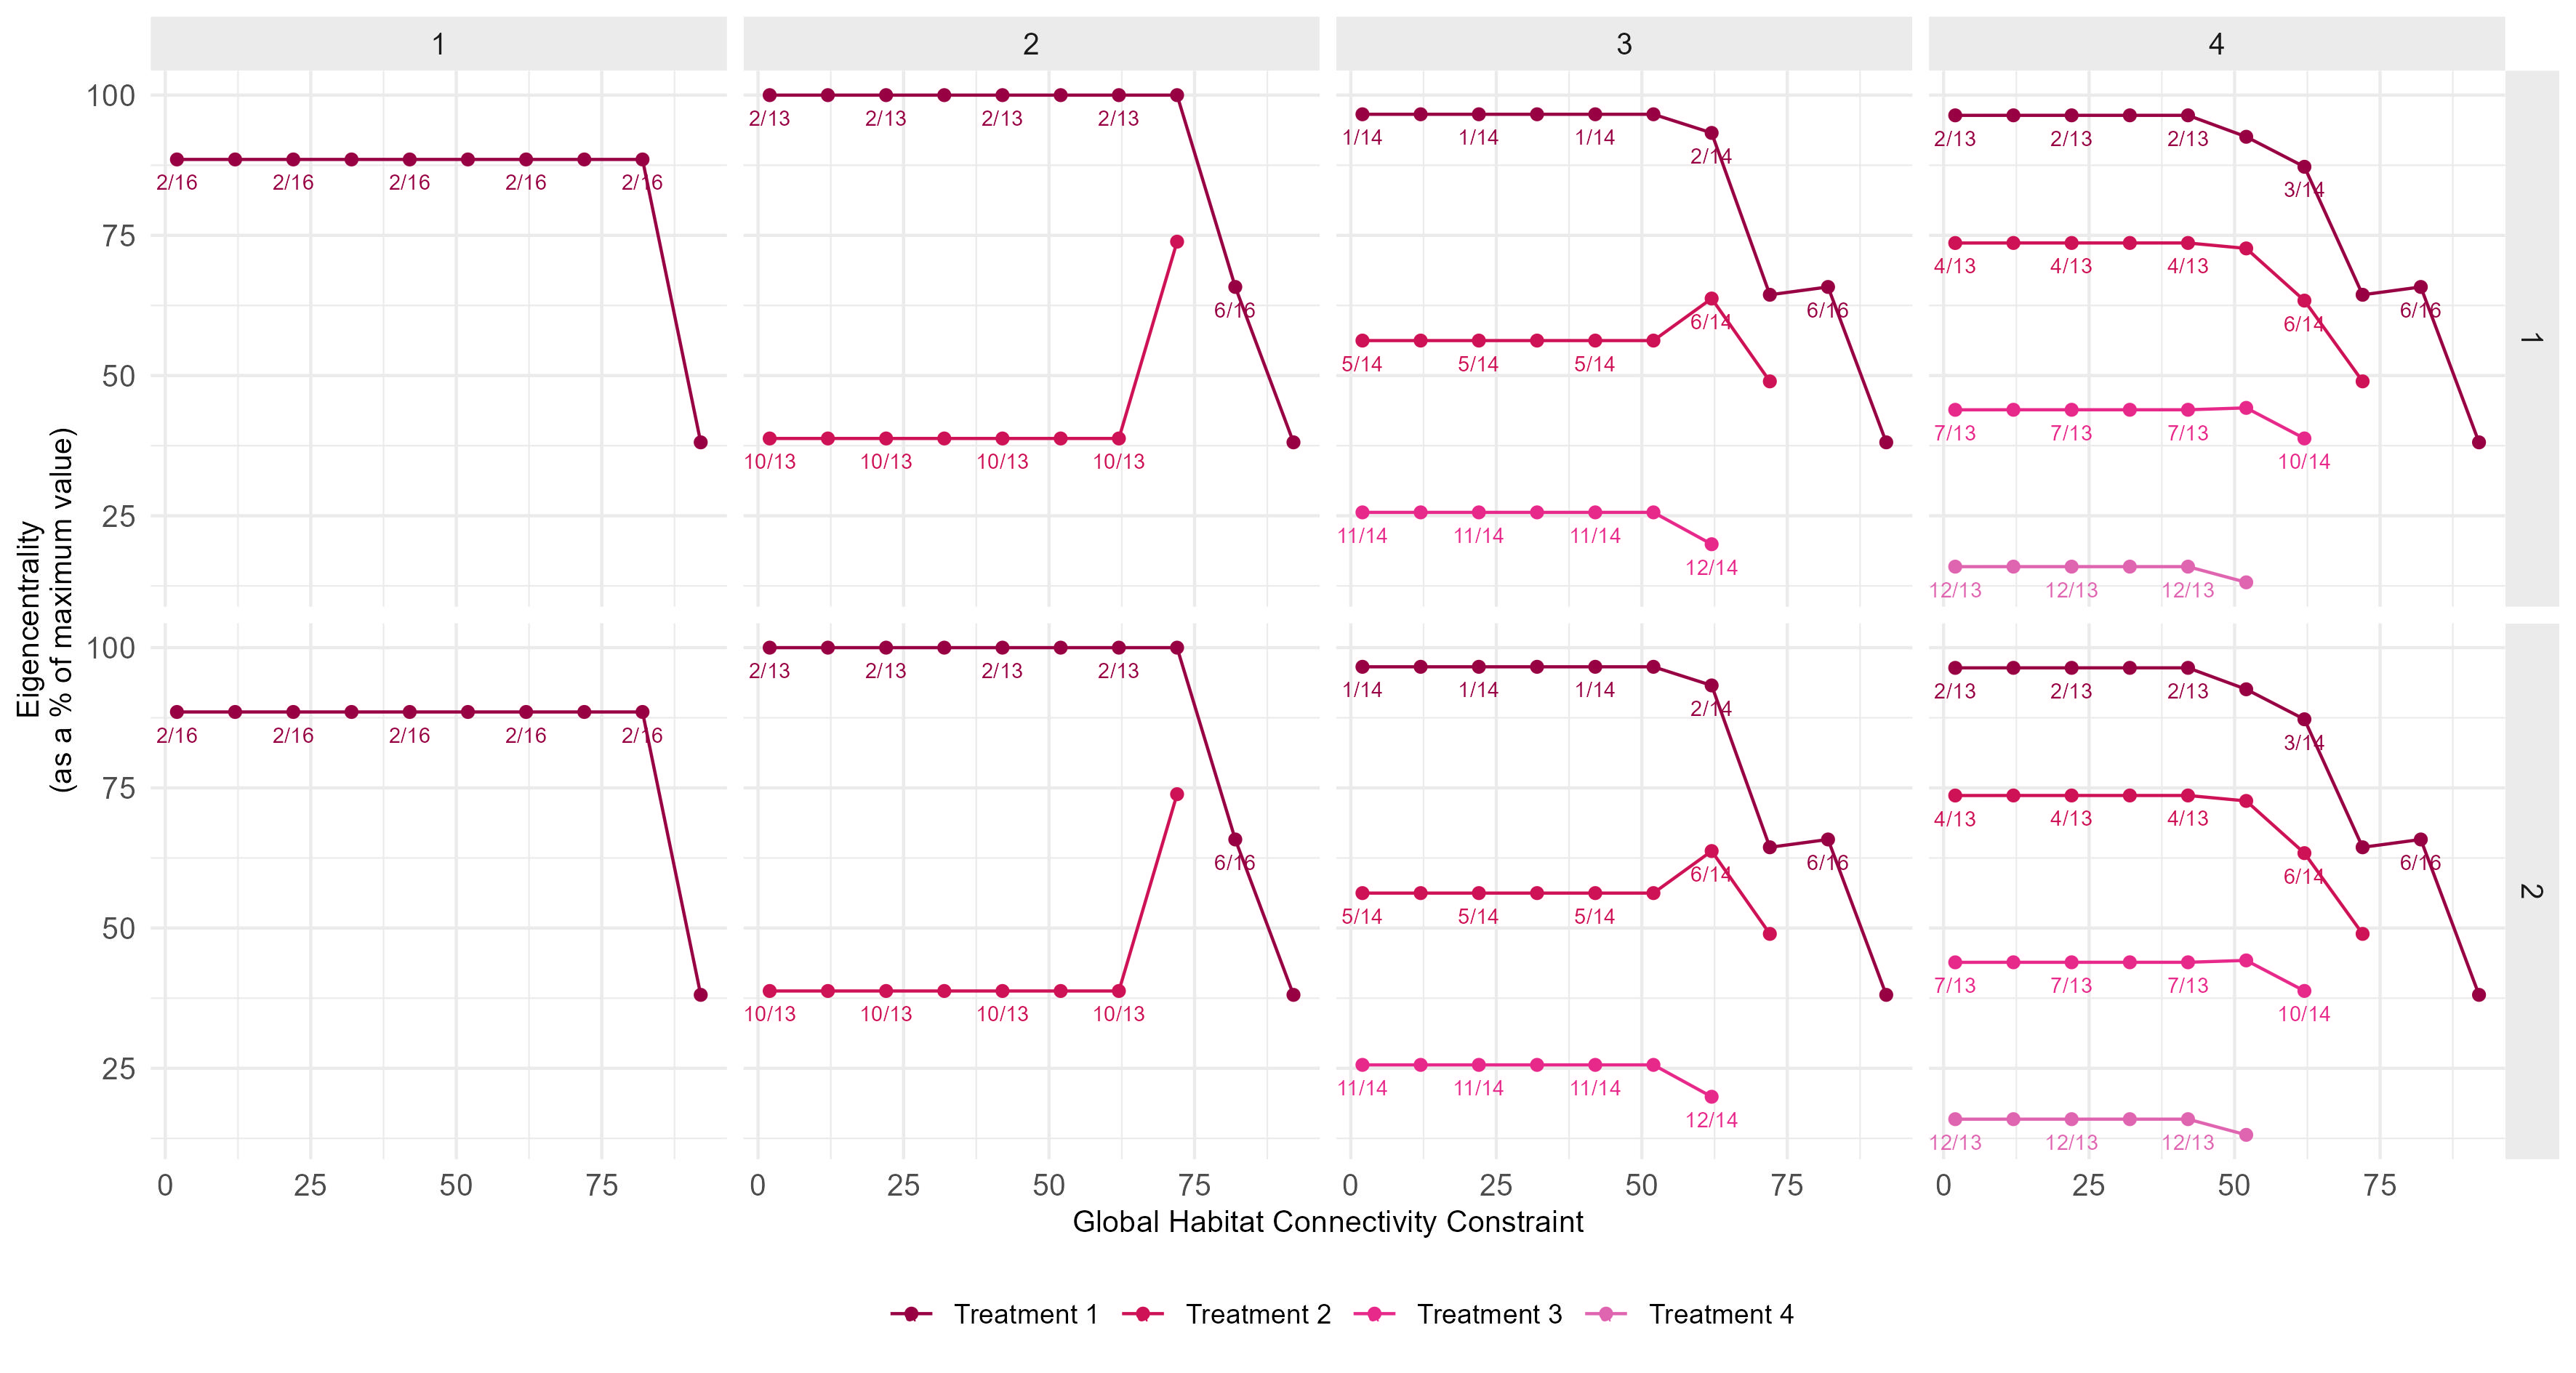
\includegraphics[width = .8\textwidth]{figures/wildland/eigencentrality_treatment.jpg}
	\caption{Eigencentrality of treated vertices (average value and rank)}
	\label{fig:eigen}
	\end{subfigure}
	\caption{Average subgraph and degree centralities, and eigencentrality, across steady-state cycles for budget and global habitat connectivity constraints}
\end{figure}
\clearpage


\begin{figure}[h]
	\centering
	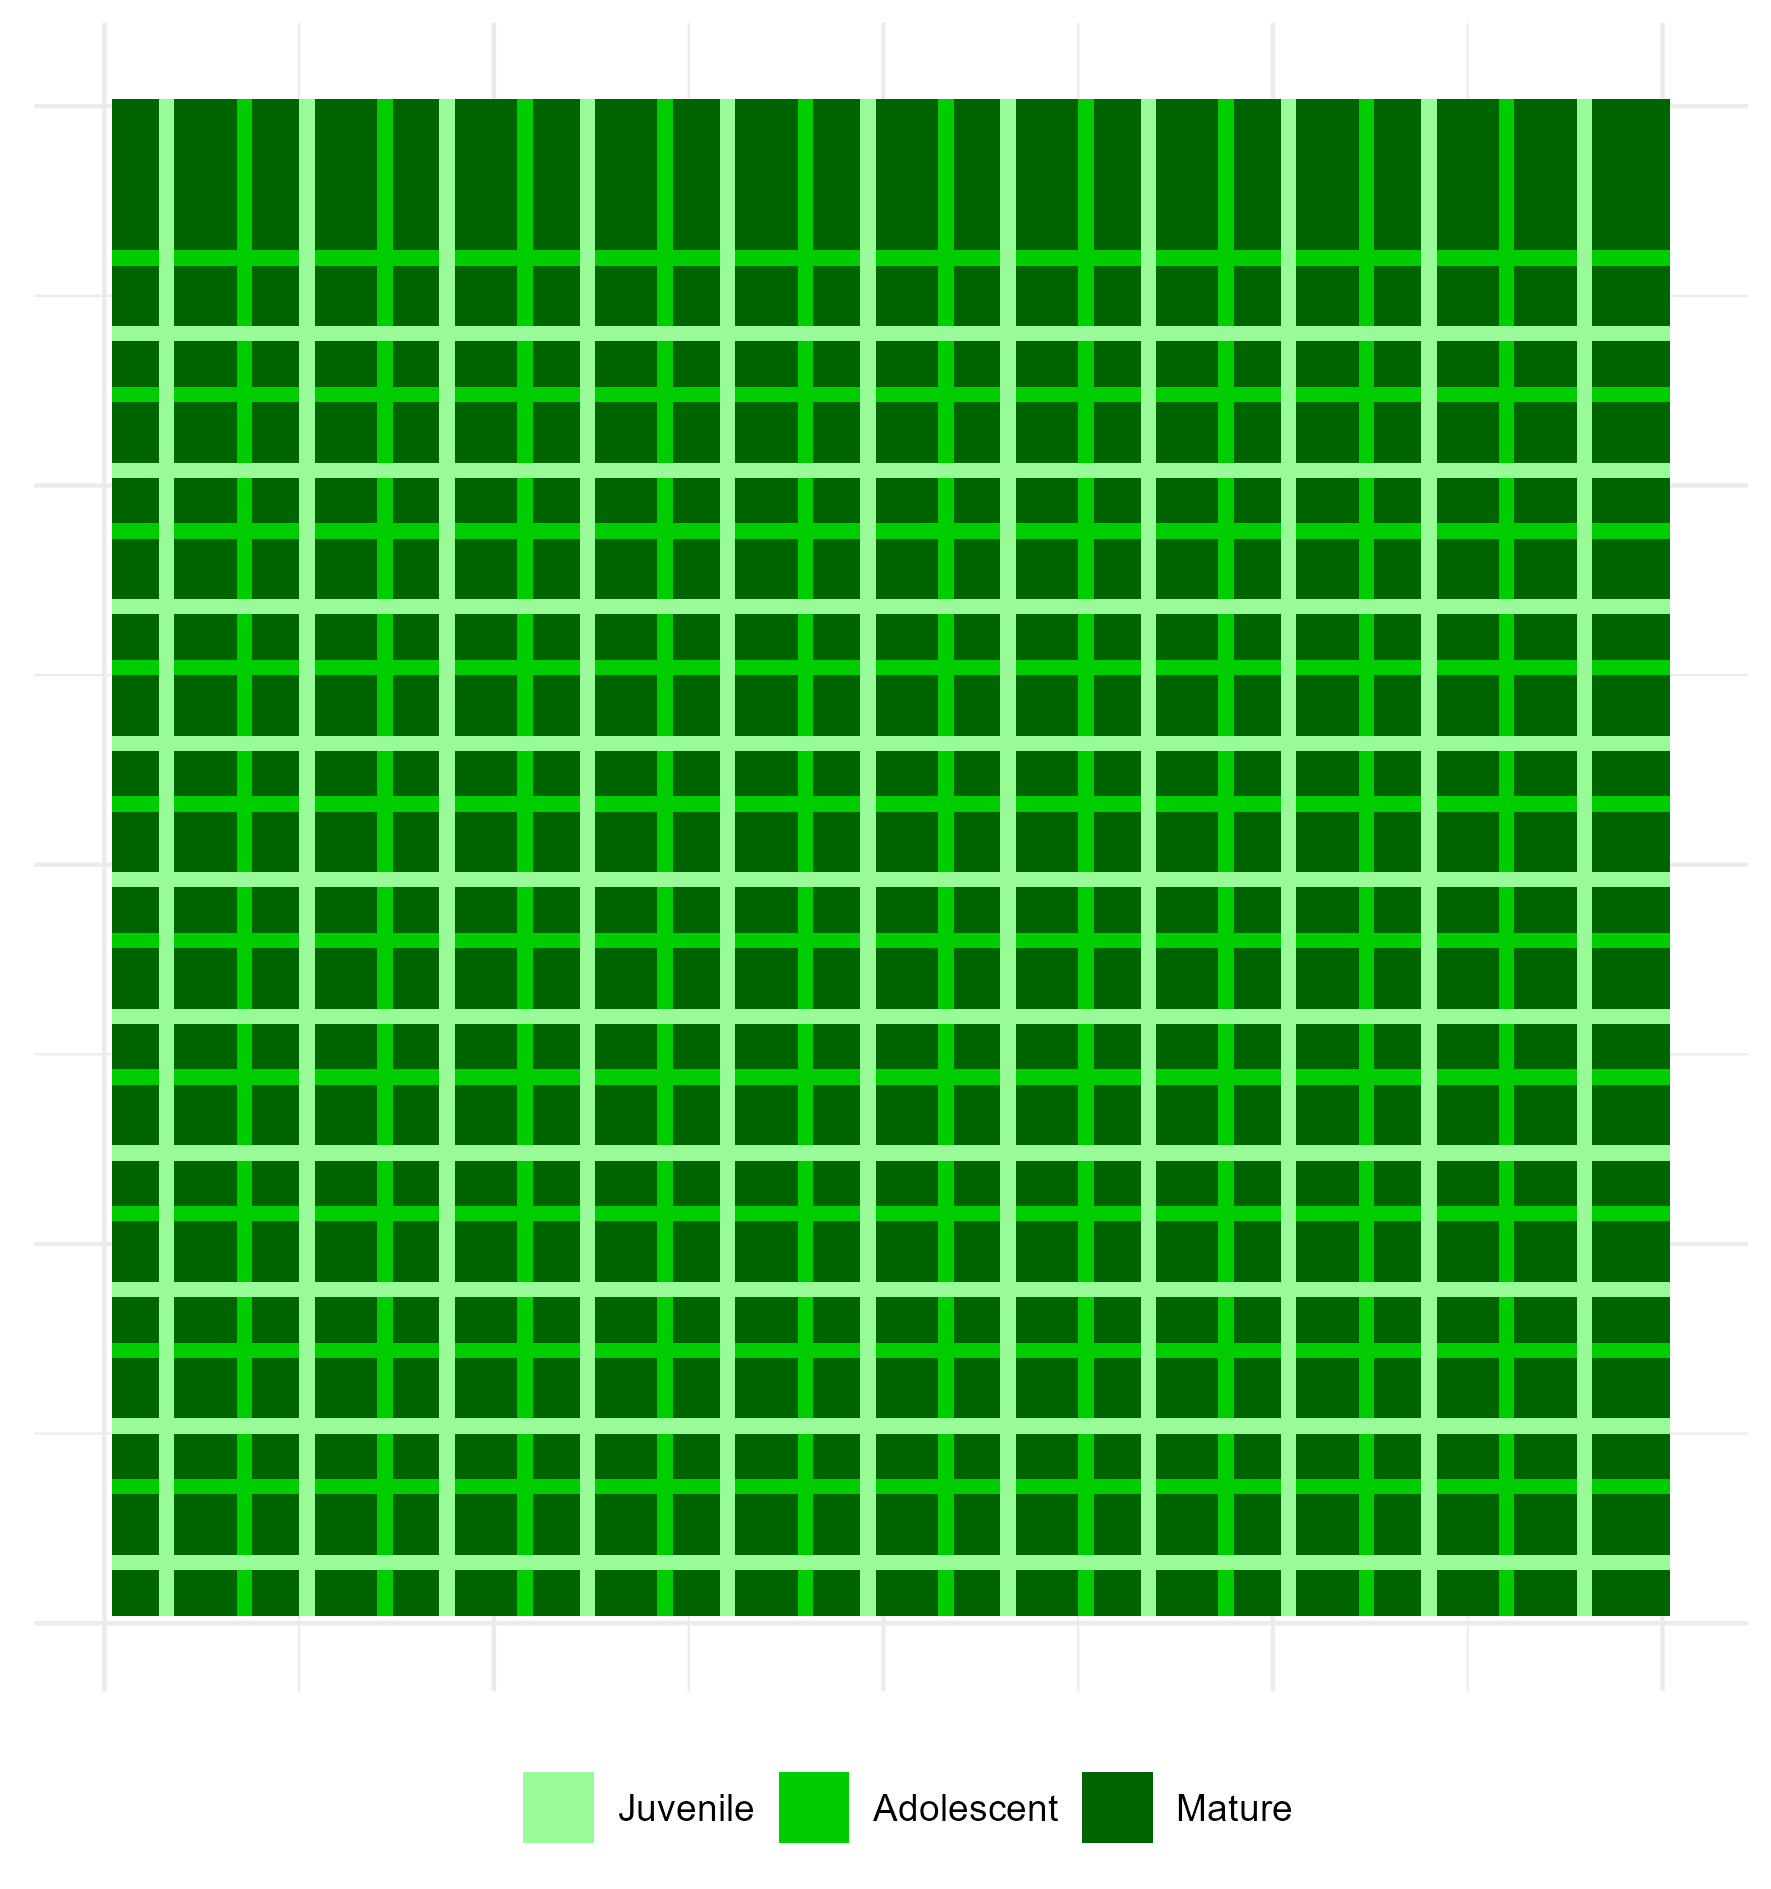
\includegraphics[width = .8\textwidth]{figures/wildland/grid_treatment.jpg}
	\caption{Illustration of grid treatment rule}
	\label{fig:grid}
\end{figure}

\begin{figure}[H]
	\centering
	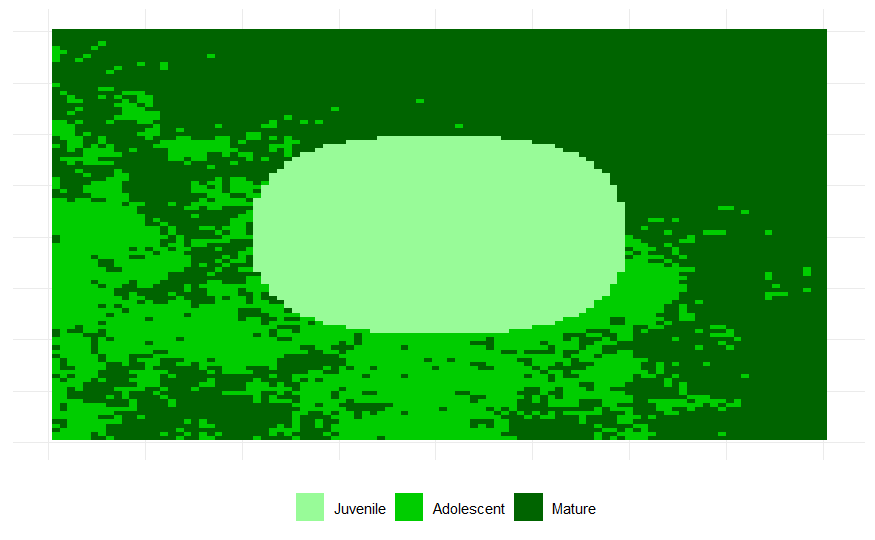
\includegraphics[width = .8\textwidth]{figures/wildland/example_adaptive_treatment.jpg}
	\caption{Example of location of treatment with adaptive policy on large scale landscape}
	\label{fig:adaptive_policy}
\end{figure}





%\begin{figure}[H]
%     \centering
%     \begin{subfigure}[b]{0.4\textwidth}
%         \centering
%         \includegraphics[width=.98\textwidth]{figures/wildland/risky_surface3.png}
%         \caption{}
%         \label{fig:indicator_surface3}
%     \end{subfigure}
%     \begin{subfigure}[b]{0.4\textwidth}
%         \centering
%         \includegraphics[width=\textwidth]{figures/wildland/risky_surface4.png}
%         \caption{}
%         \label{fig:indicator_surface4}
%     \end{subfigure}
%     \hfill
%     \begin{subfigure}[b]{0.4\textwidth}
%         \centering
%         \includegraphics[width=\textwidth]{figures/wildland/risky_components3.png}
%         \caption{}
%         \label{fig:indicator_component3}
%     \end{subfigure}
%     \begin{subfigure}[b]{0.4\textwidth}
%         \centering
%         \includegraphics[width=.98\textwidth]{figures/wildland/risky_component4.png}
%         \caption{}
%         \label{fig:indicator_component4}
%     \end{subfigure}
%     \hfill
%          \begin{subfigure}[b]{0.4\textwidth}
%         \centering
%         \includegraphics[width=.98\textwidth]{figures/wildland/%max_component_area3.png}
%         \caption{}
%         \label{fig:indicator_component3}
%     \end{subfigure}
%     \begin{subfigure}[b]{0.4\textwidth}
%         \centering
%         \includegraphics[width=\textwidth]{figures/wildland/%max_component_area4.png}
%         \caption{}
%         \label{fig:indicator_component4}
%     \end{subfigure}
%        \caption{Assessment: surface, components of high-risk graph (95\% CI %shaded)}
%        \label{fig:indicators_1}
%\end{figure}
%\newpage

%\begin{figure}[H]
%    \centering
%    \includegraphics[width=0.45\textwidth]{squelette_draft/graphs_manuscript/risky_surface3.png} 
%    \includegraphics[width=0.45\textwidth]{squelette_draft/graphs_manuscript/risky_surface4.png}\\
%    \includegraphics[width=0.45\textwidth]{squelette_draft/graphs_manuscript/risky_components3.png}
%    \includegraphics[width=0.45\textwidth]{squelette_draft/graphs_manuscript/risky_component4.png}\\
%    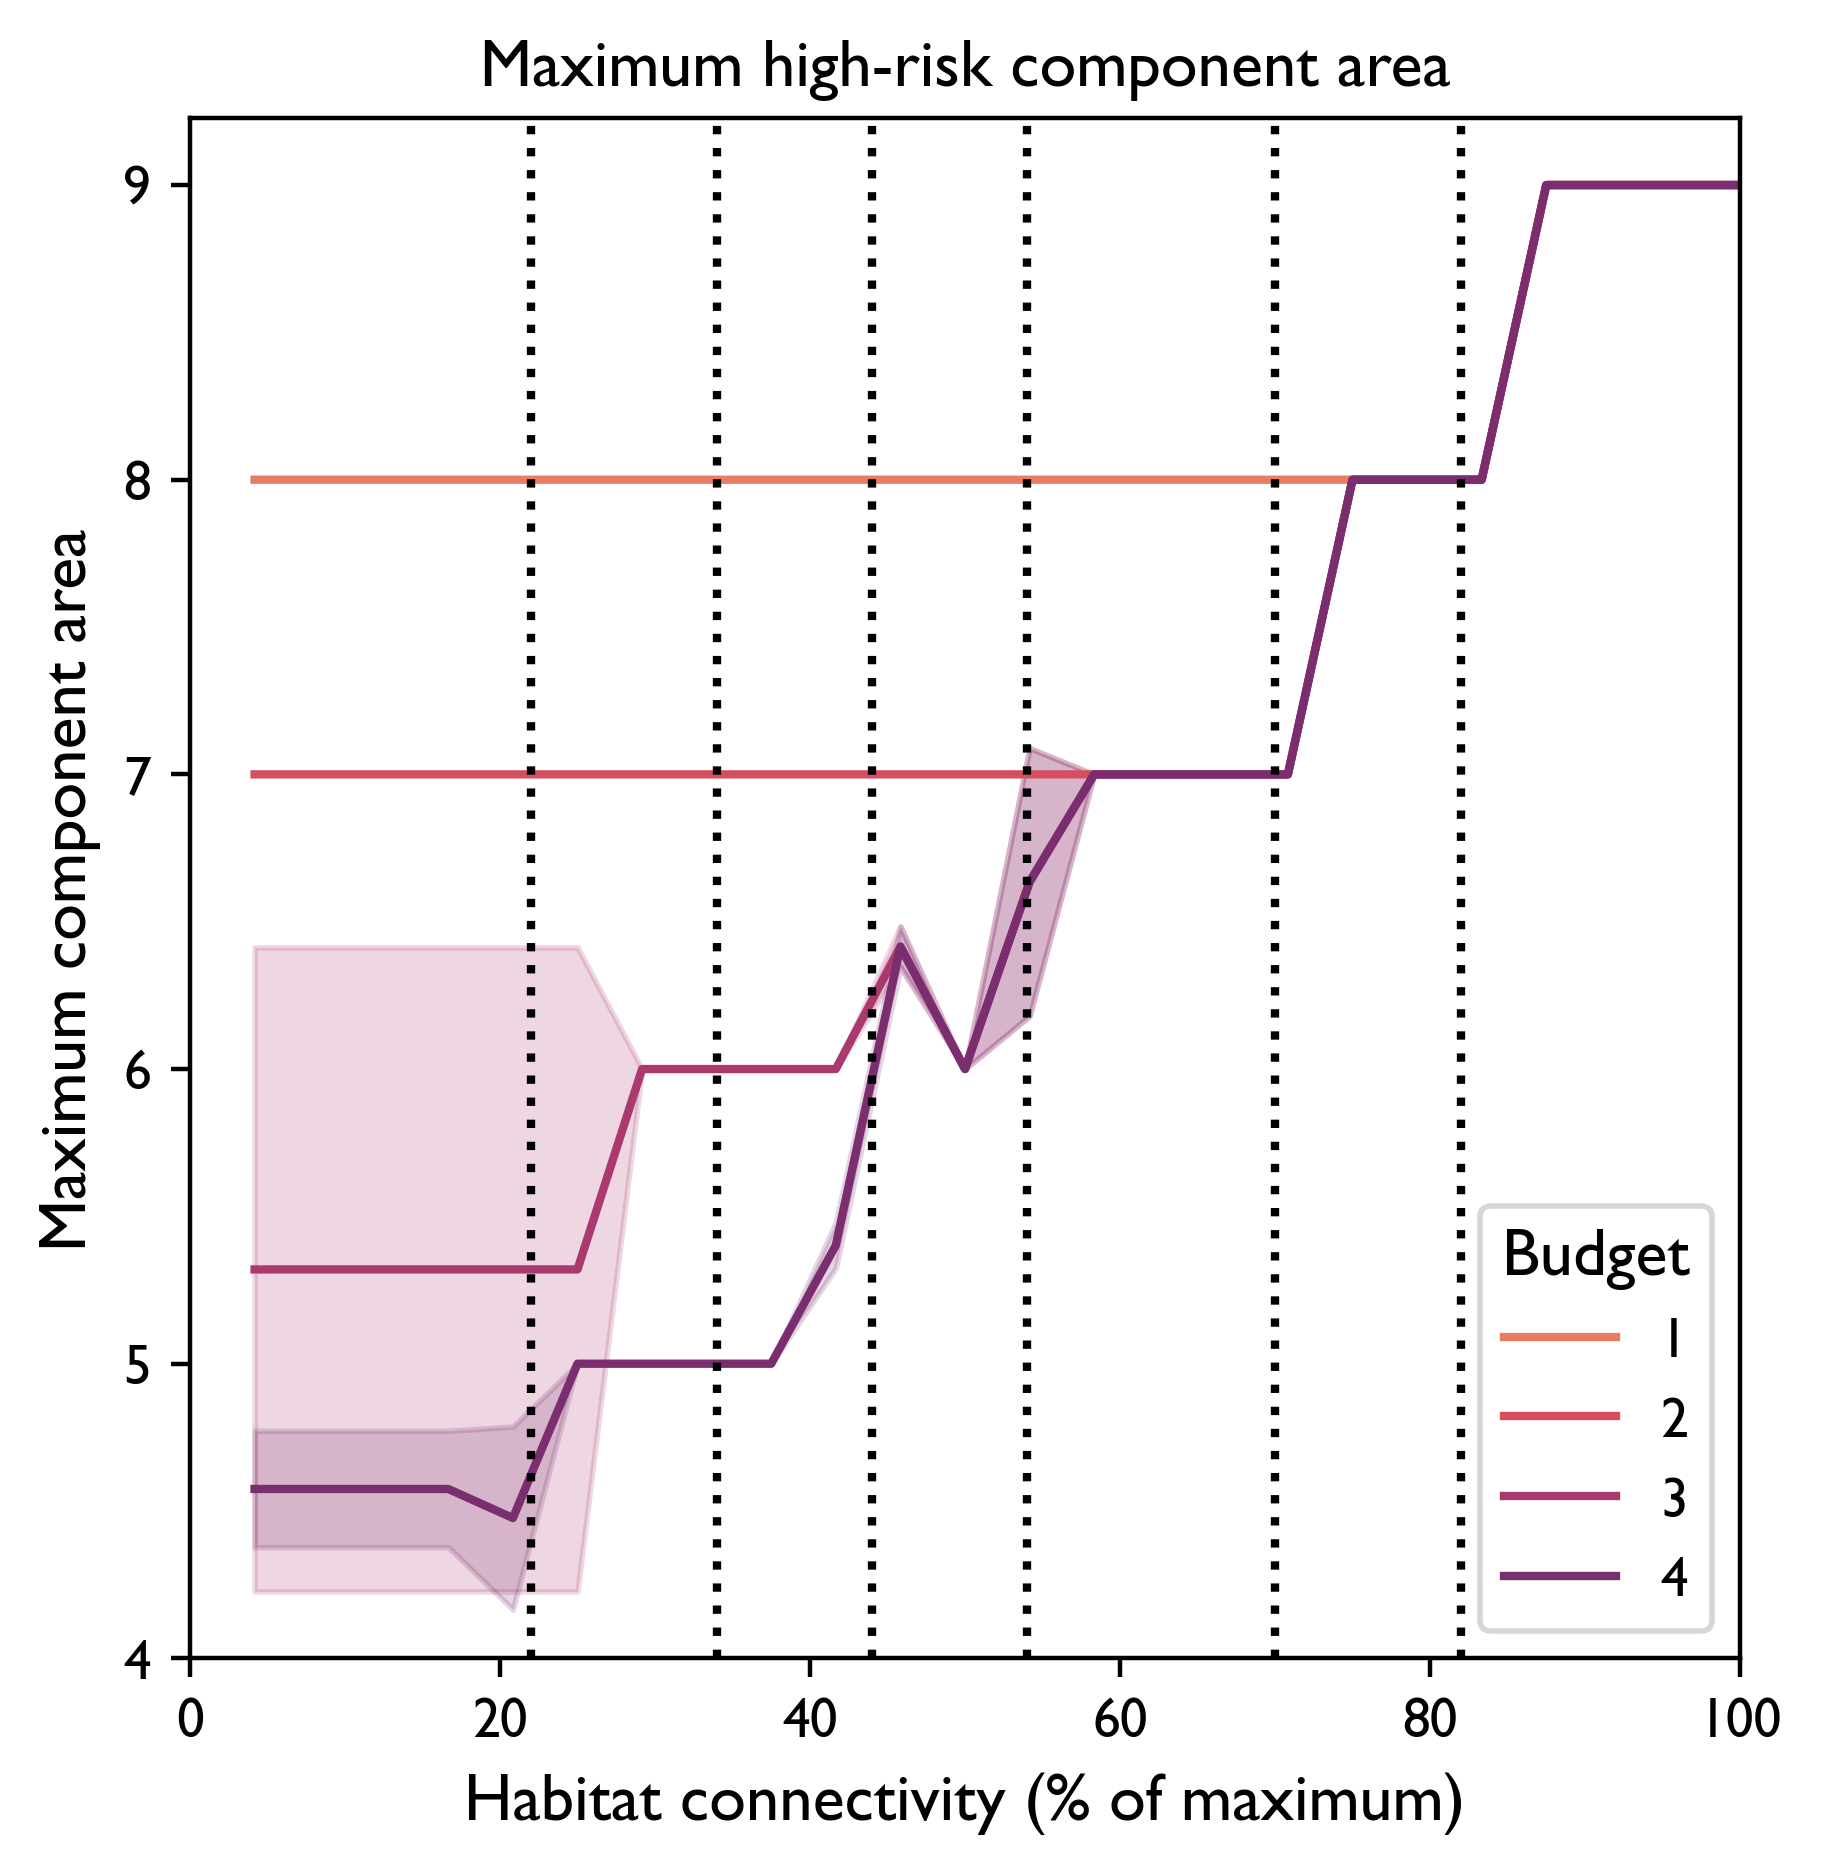
\includegraphics[width=0.45\textwidth]{squelette_draft/graphs_manuscript/max_component_area3.png} 
%    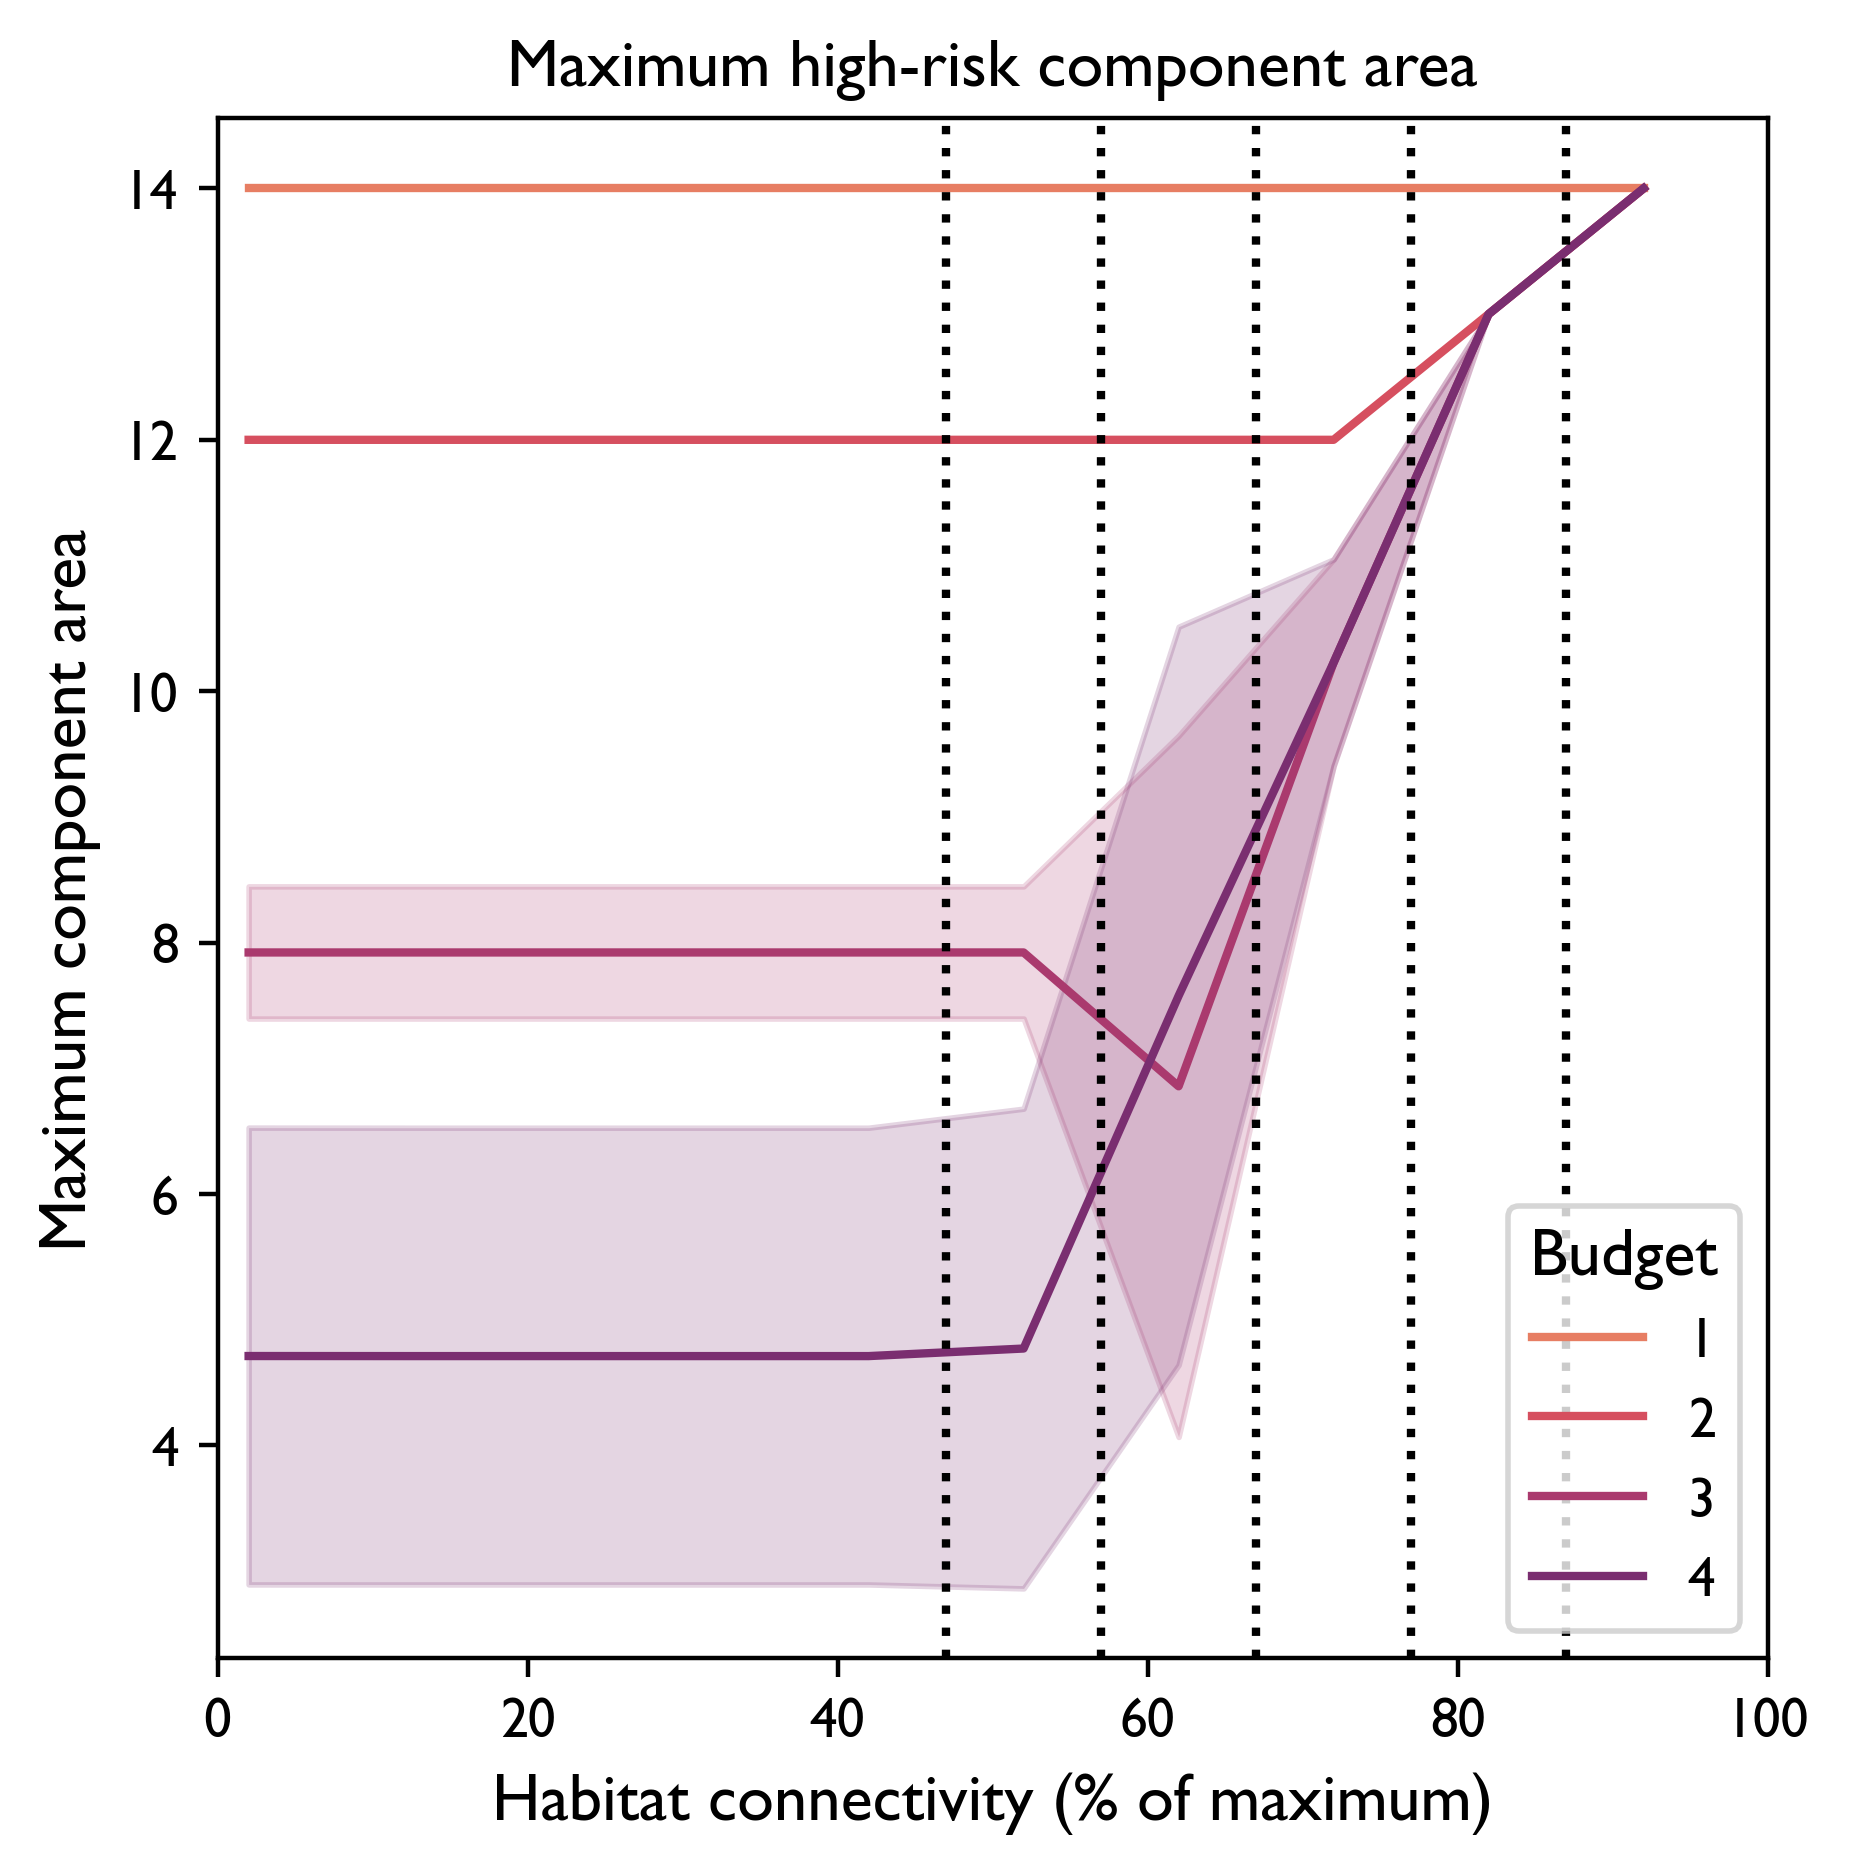
\includegraphics[width=0.45\textwidth]{squelette_draft/graphs_manuscript/max_component_area4.png} 
%    \caption{Assessment indicators: surface and components of high-risk graph}
%    \label{fig:indicators_1}
%\end{figure}

%\begin{figure}[H]
%     \centering
%     \begin{subfigure}[b]{0.4\textwidth}
%         \centering
%         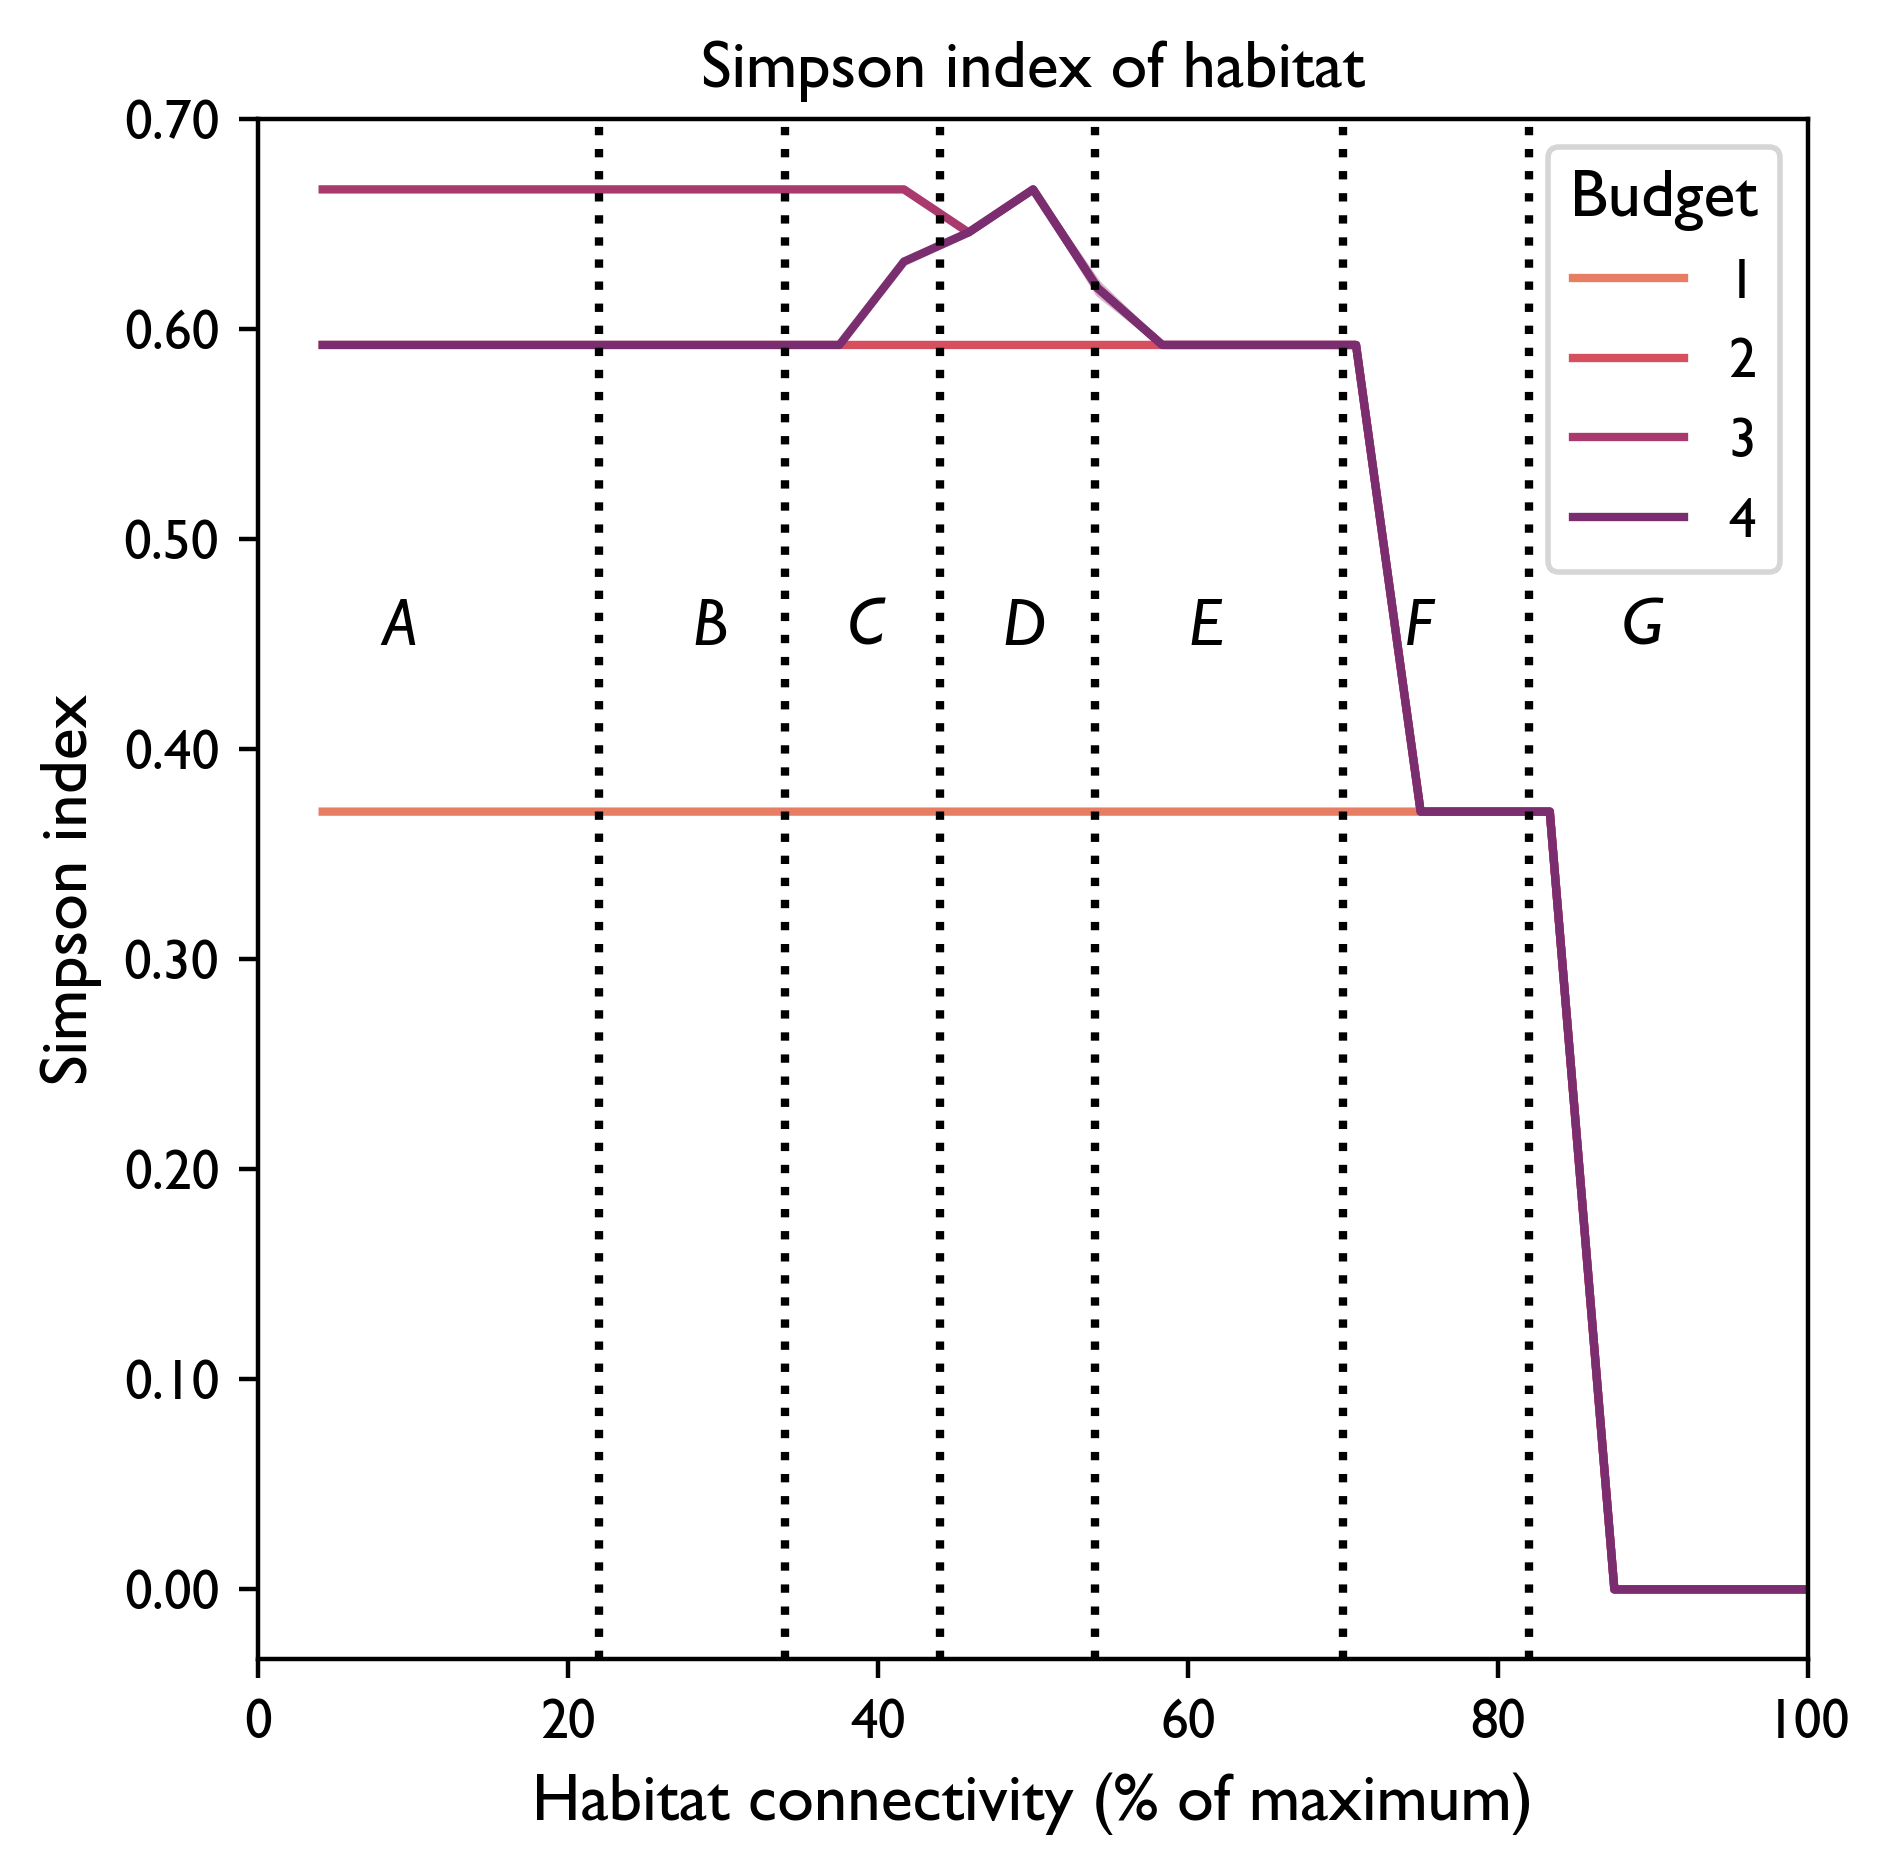
\includegraphics[width=\textwidth]{figures/wildland/simpson_index3.png}
%         \caption{}
%         \label{fig:indicator_simpson3}
%     \end{subfigure}
%    \begin{subfigure}[b]{0.4\textwidth}
%         \centering
%         \includegraphics[width=.985\textwidth]{figures/wildland/%simpson_index4.png}
%         \caption{}
%         \label{fig:indicator_simpson4}
%    \end{subfigure}
%    \hfill
%     \begin{subfigure}[b]{0.4\textwidth}
%         \centering
%         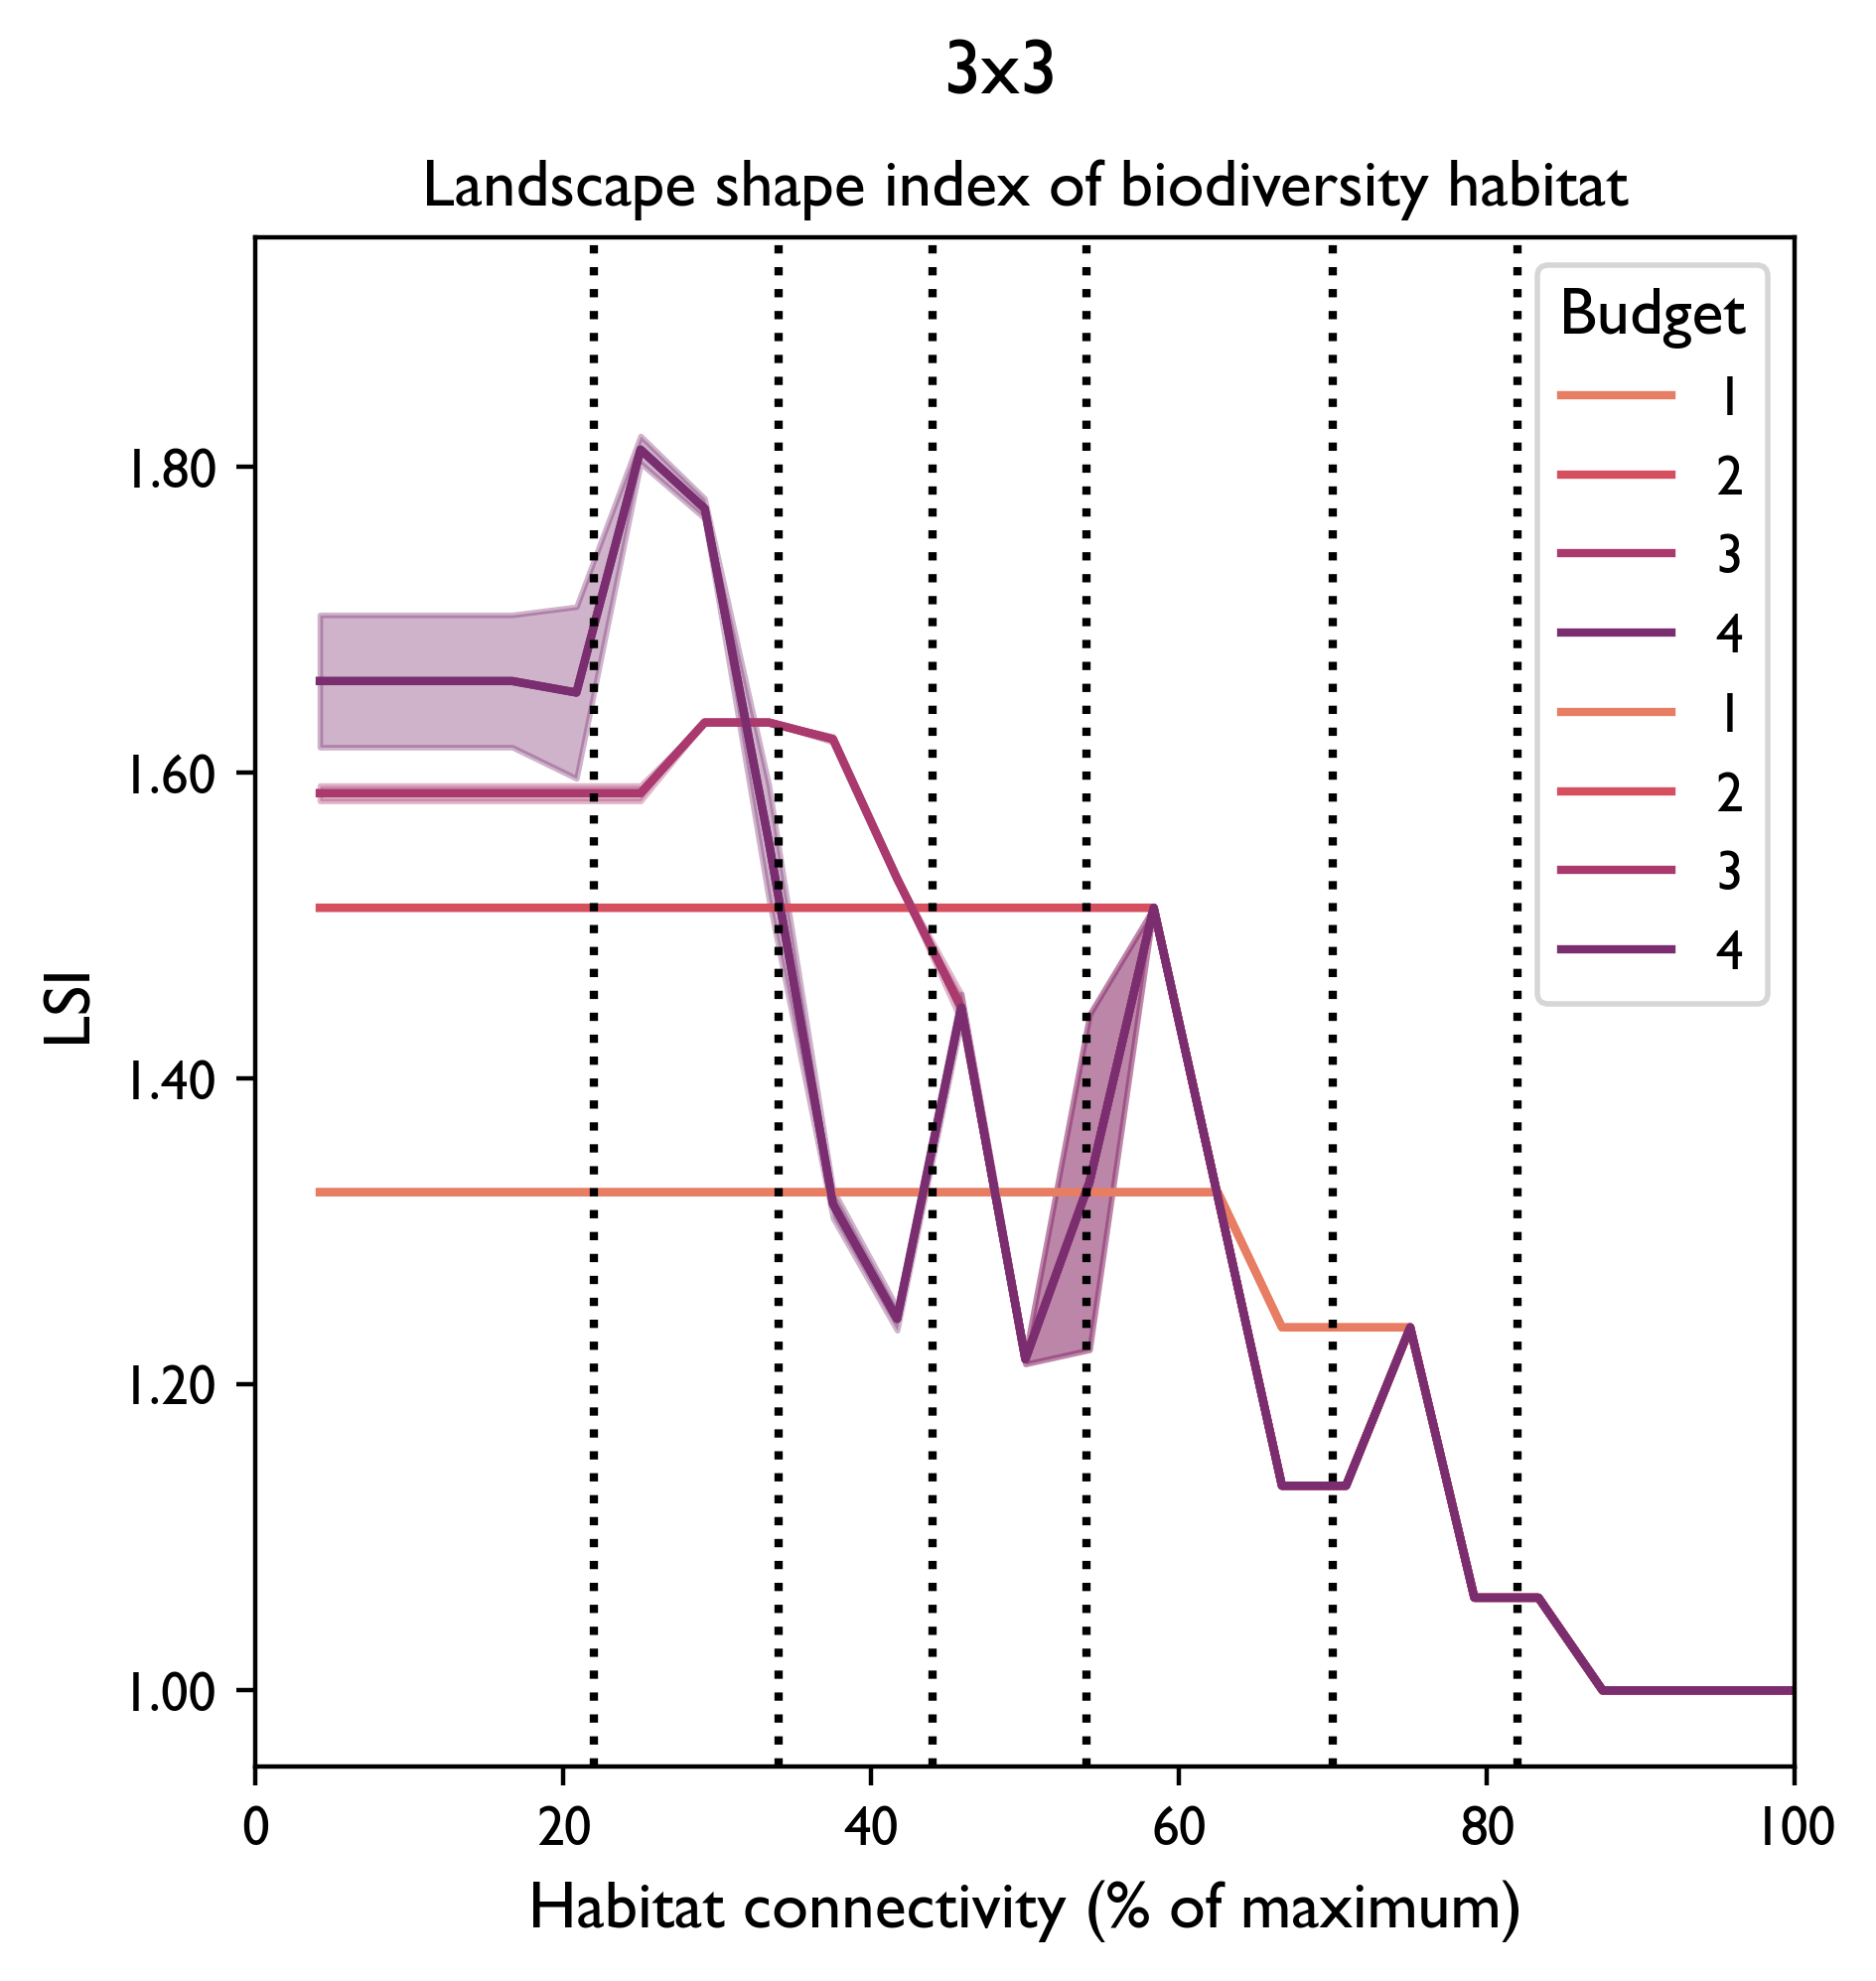
\includegraphics[width=\textwidth]{figures/wildland/LSI_biod3.png}
%         \caption{}
%         \label{fig:indicator_LSI3}
%     \end{subfigure}
%     \begin{subfigure}[b]{0.4\textwidth}
%         \centering
%         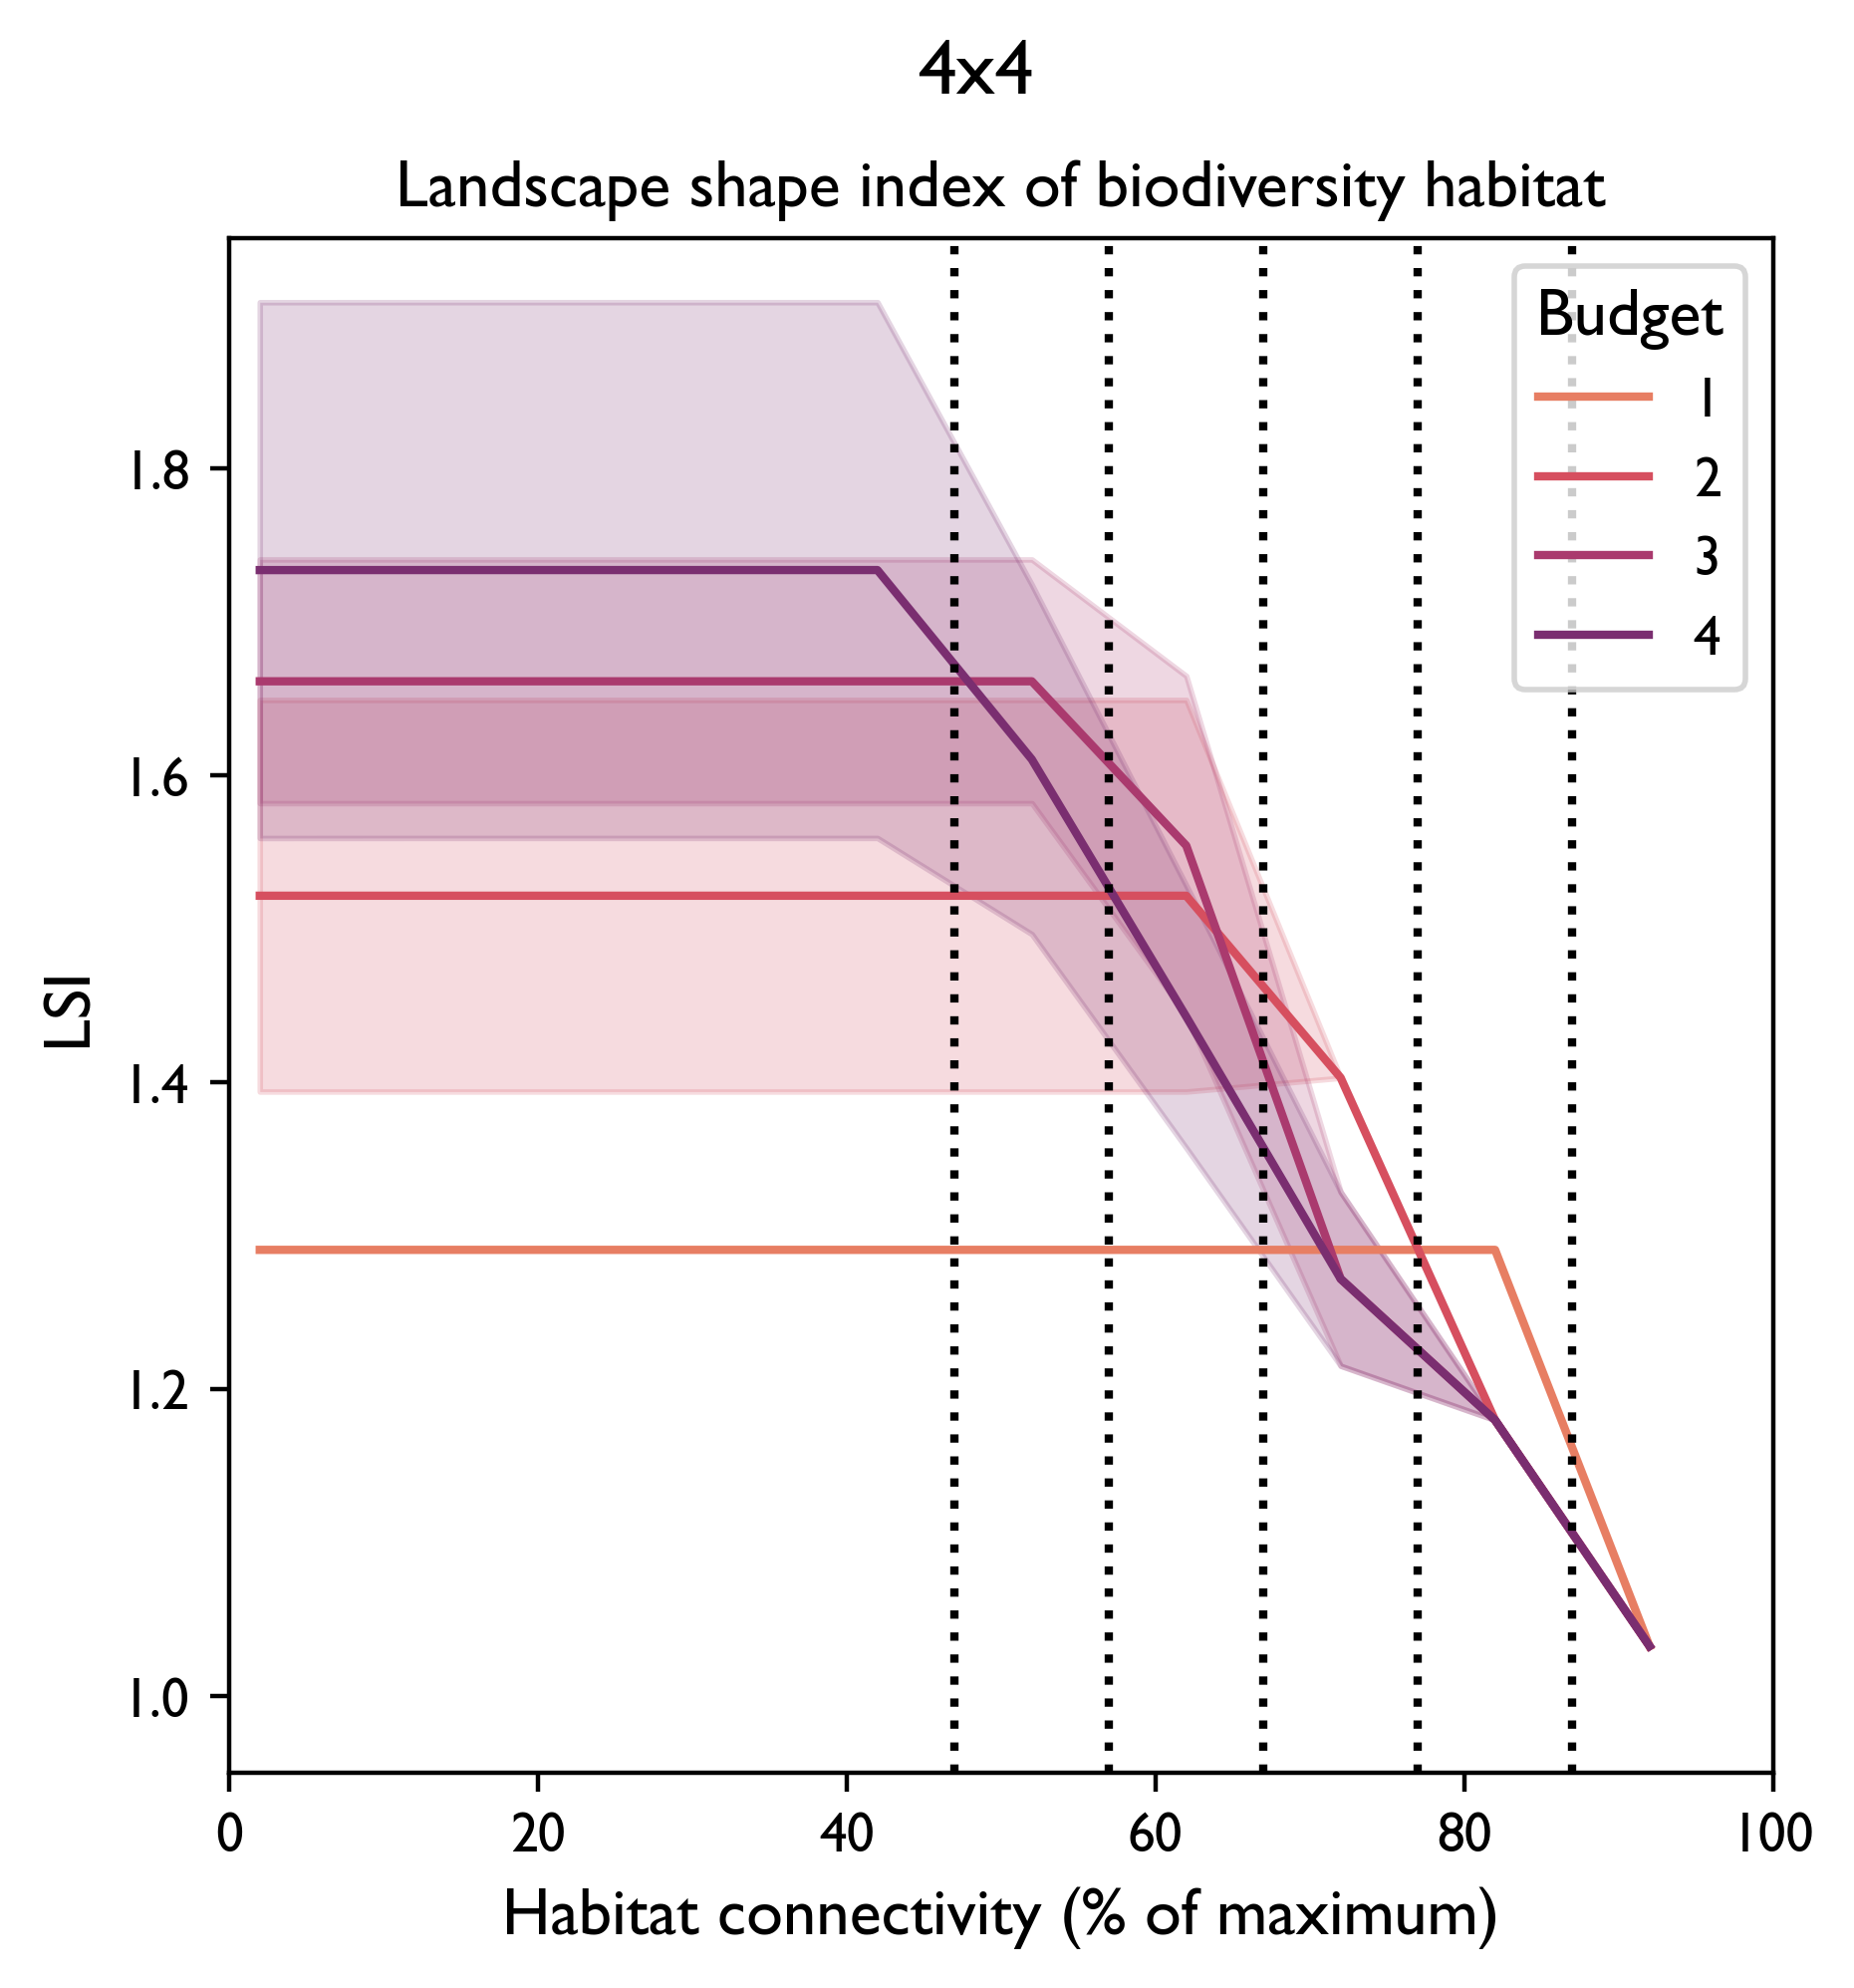
\includegraphics[width=.985\textwidth]{figures/wildland/LSI_biod4.png}
%         \caption{}
%         \label{fig:indicator_LSI4}
%     \end{subfigure}    
%    \hfill
%    \begin{subfigure}[b]{0.4\textwidth}
%         \centering
%         \includegraphics[width=\textwidth]{figures/wildland/%diversity_index3.png}
%         \caption{}
%         \label{fig:indicator_diversity3}
%     \end{subfigure}
%    \begin{subfigure}[b]{0.4\textwidth}
%         \centering
%         \includegraphics[width=0.955\textwidth]{figures/wildland/%diversity_index4.png}
%%         \caption{}
%         \label{fig:indicator_diversity4}
%    \end{subfigure}
%        \caption{Assessment: diversity (95\% CI shaded)}
%        \label{fig:indicators_2}
%\end{figure}
%\newpage


% Treatments 
%\begin{figure}[H]
%     \centering
%     \begin{subfigure}[b]{0.48\textwidth}
%         \centering
%         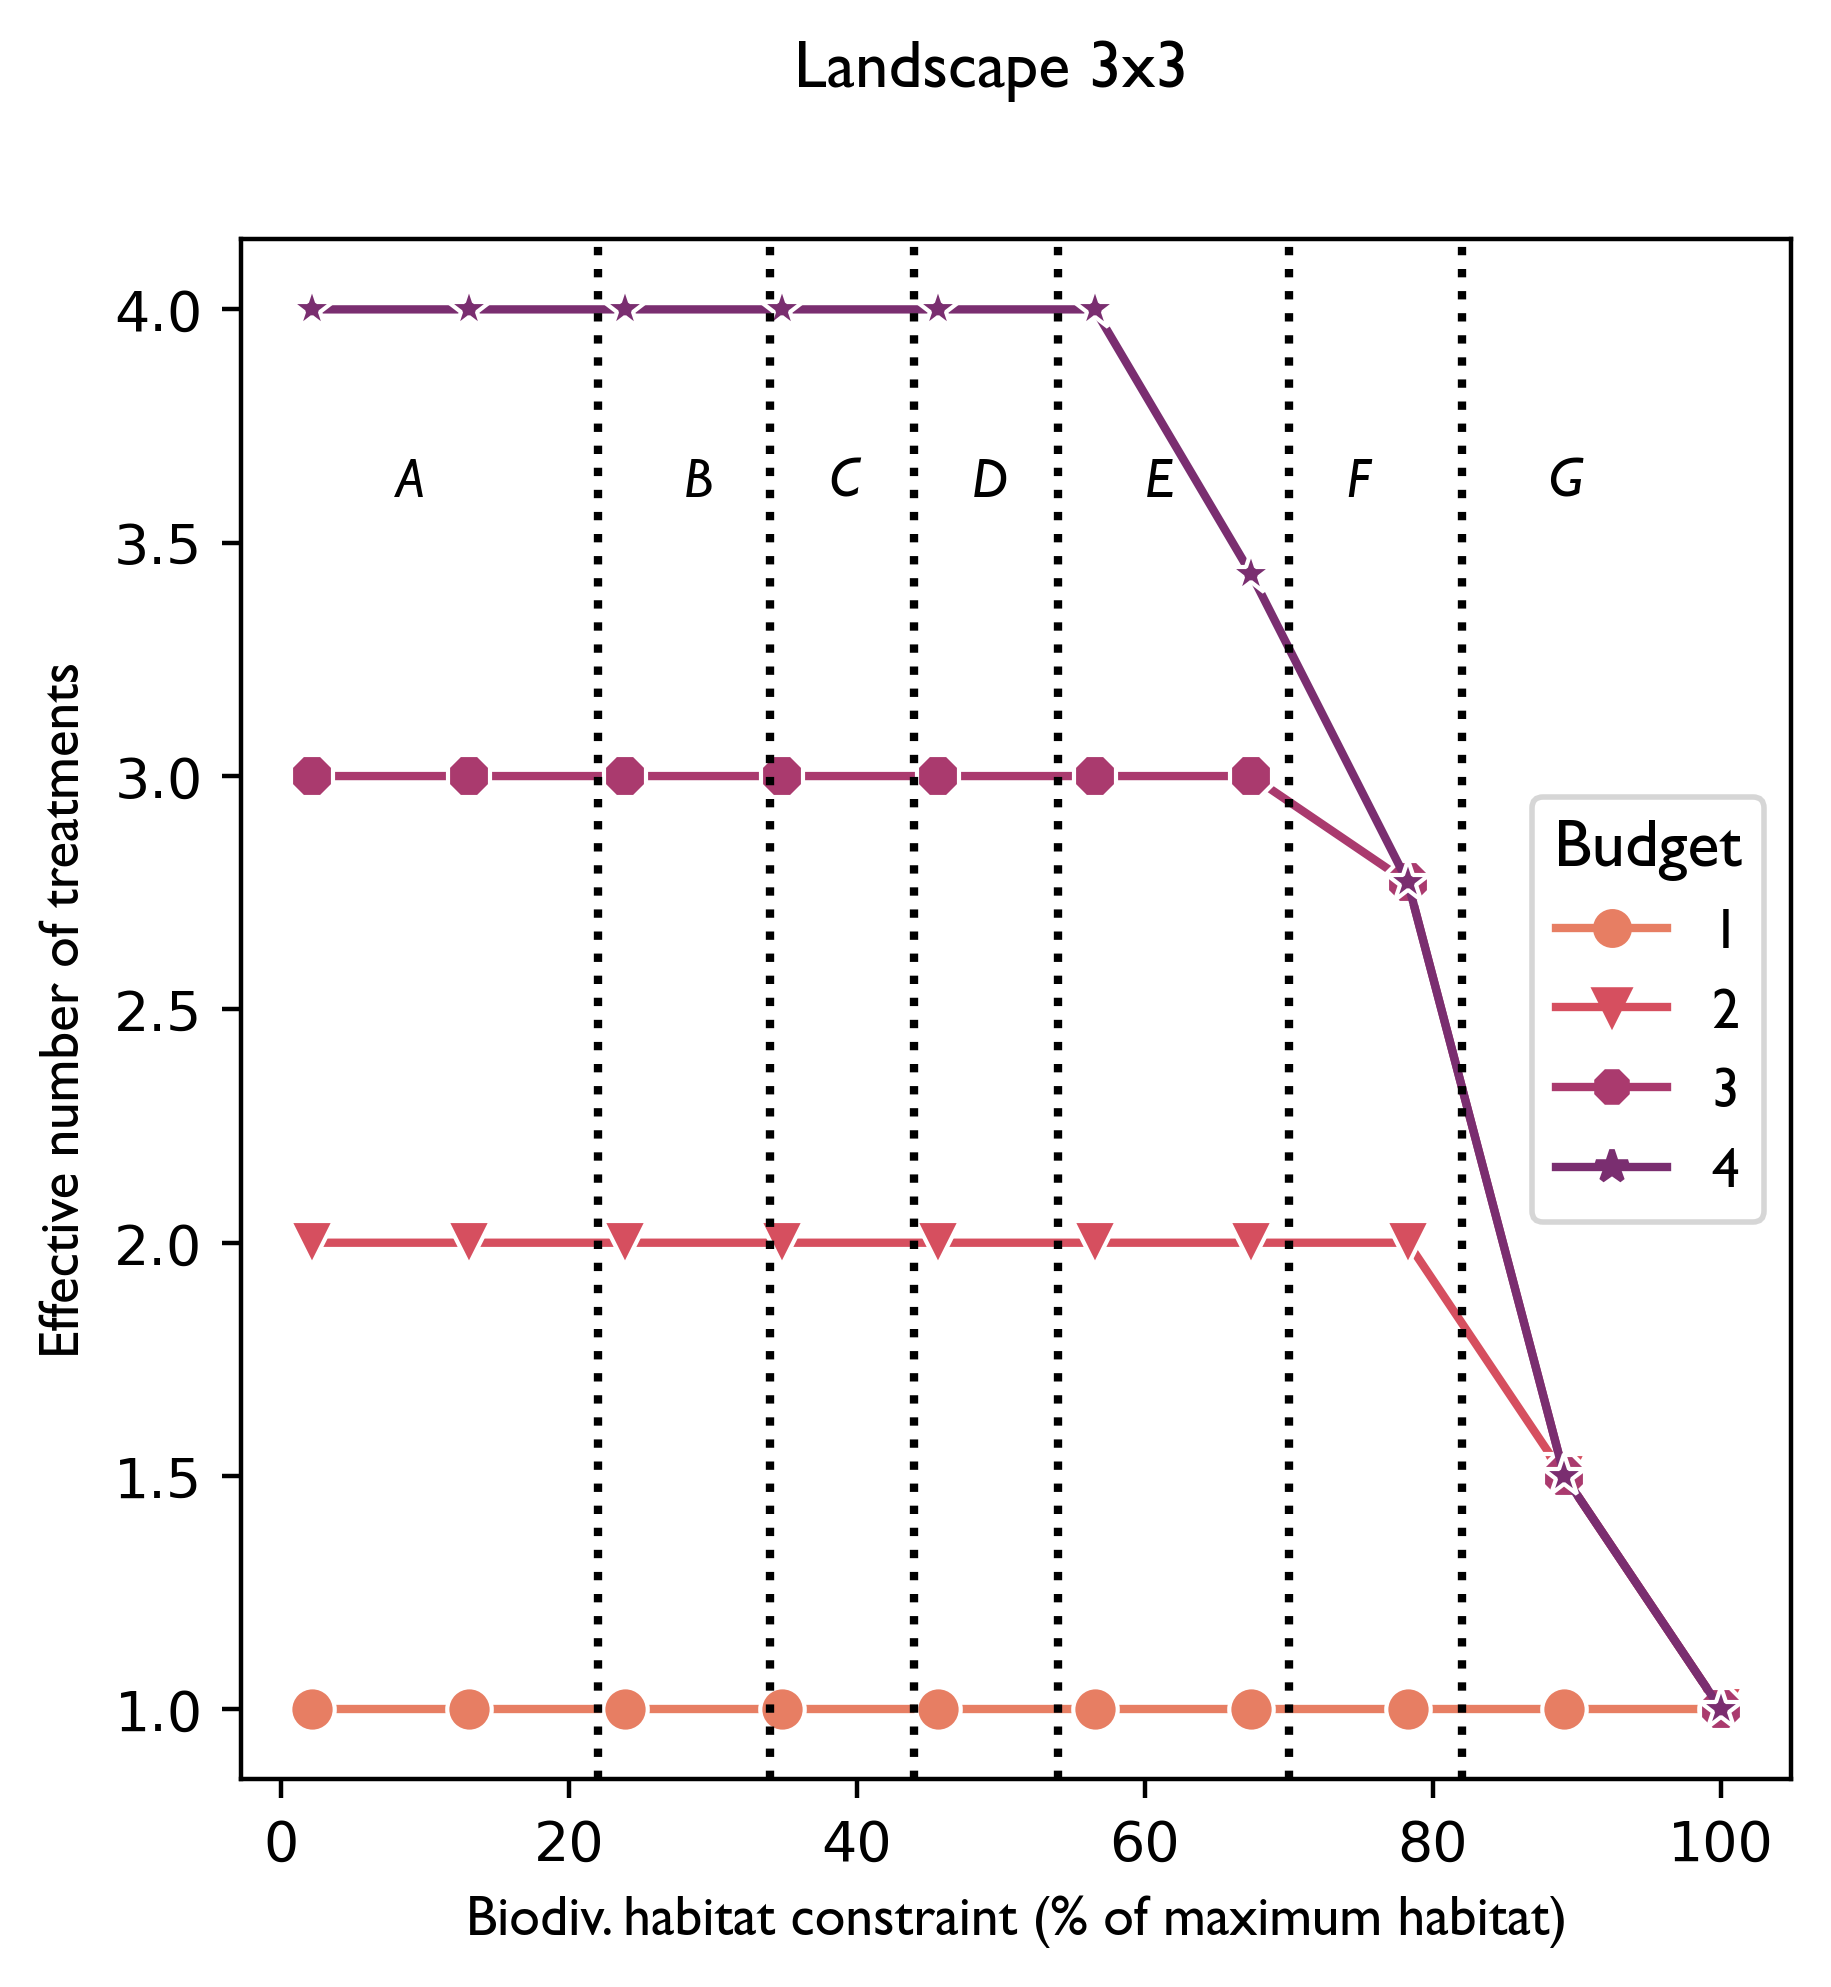
\includegraphics[width=\textwidth]{figures/wildland/number_treatments3.png}
%         \caption{}
%         \label{fig:treatments_number3}
%     \end{subfigure}
%    \begin{subfigure}[b]{0.48\textwidth}
%         \centering
%         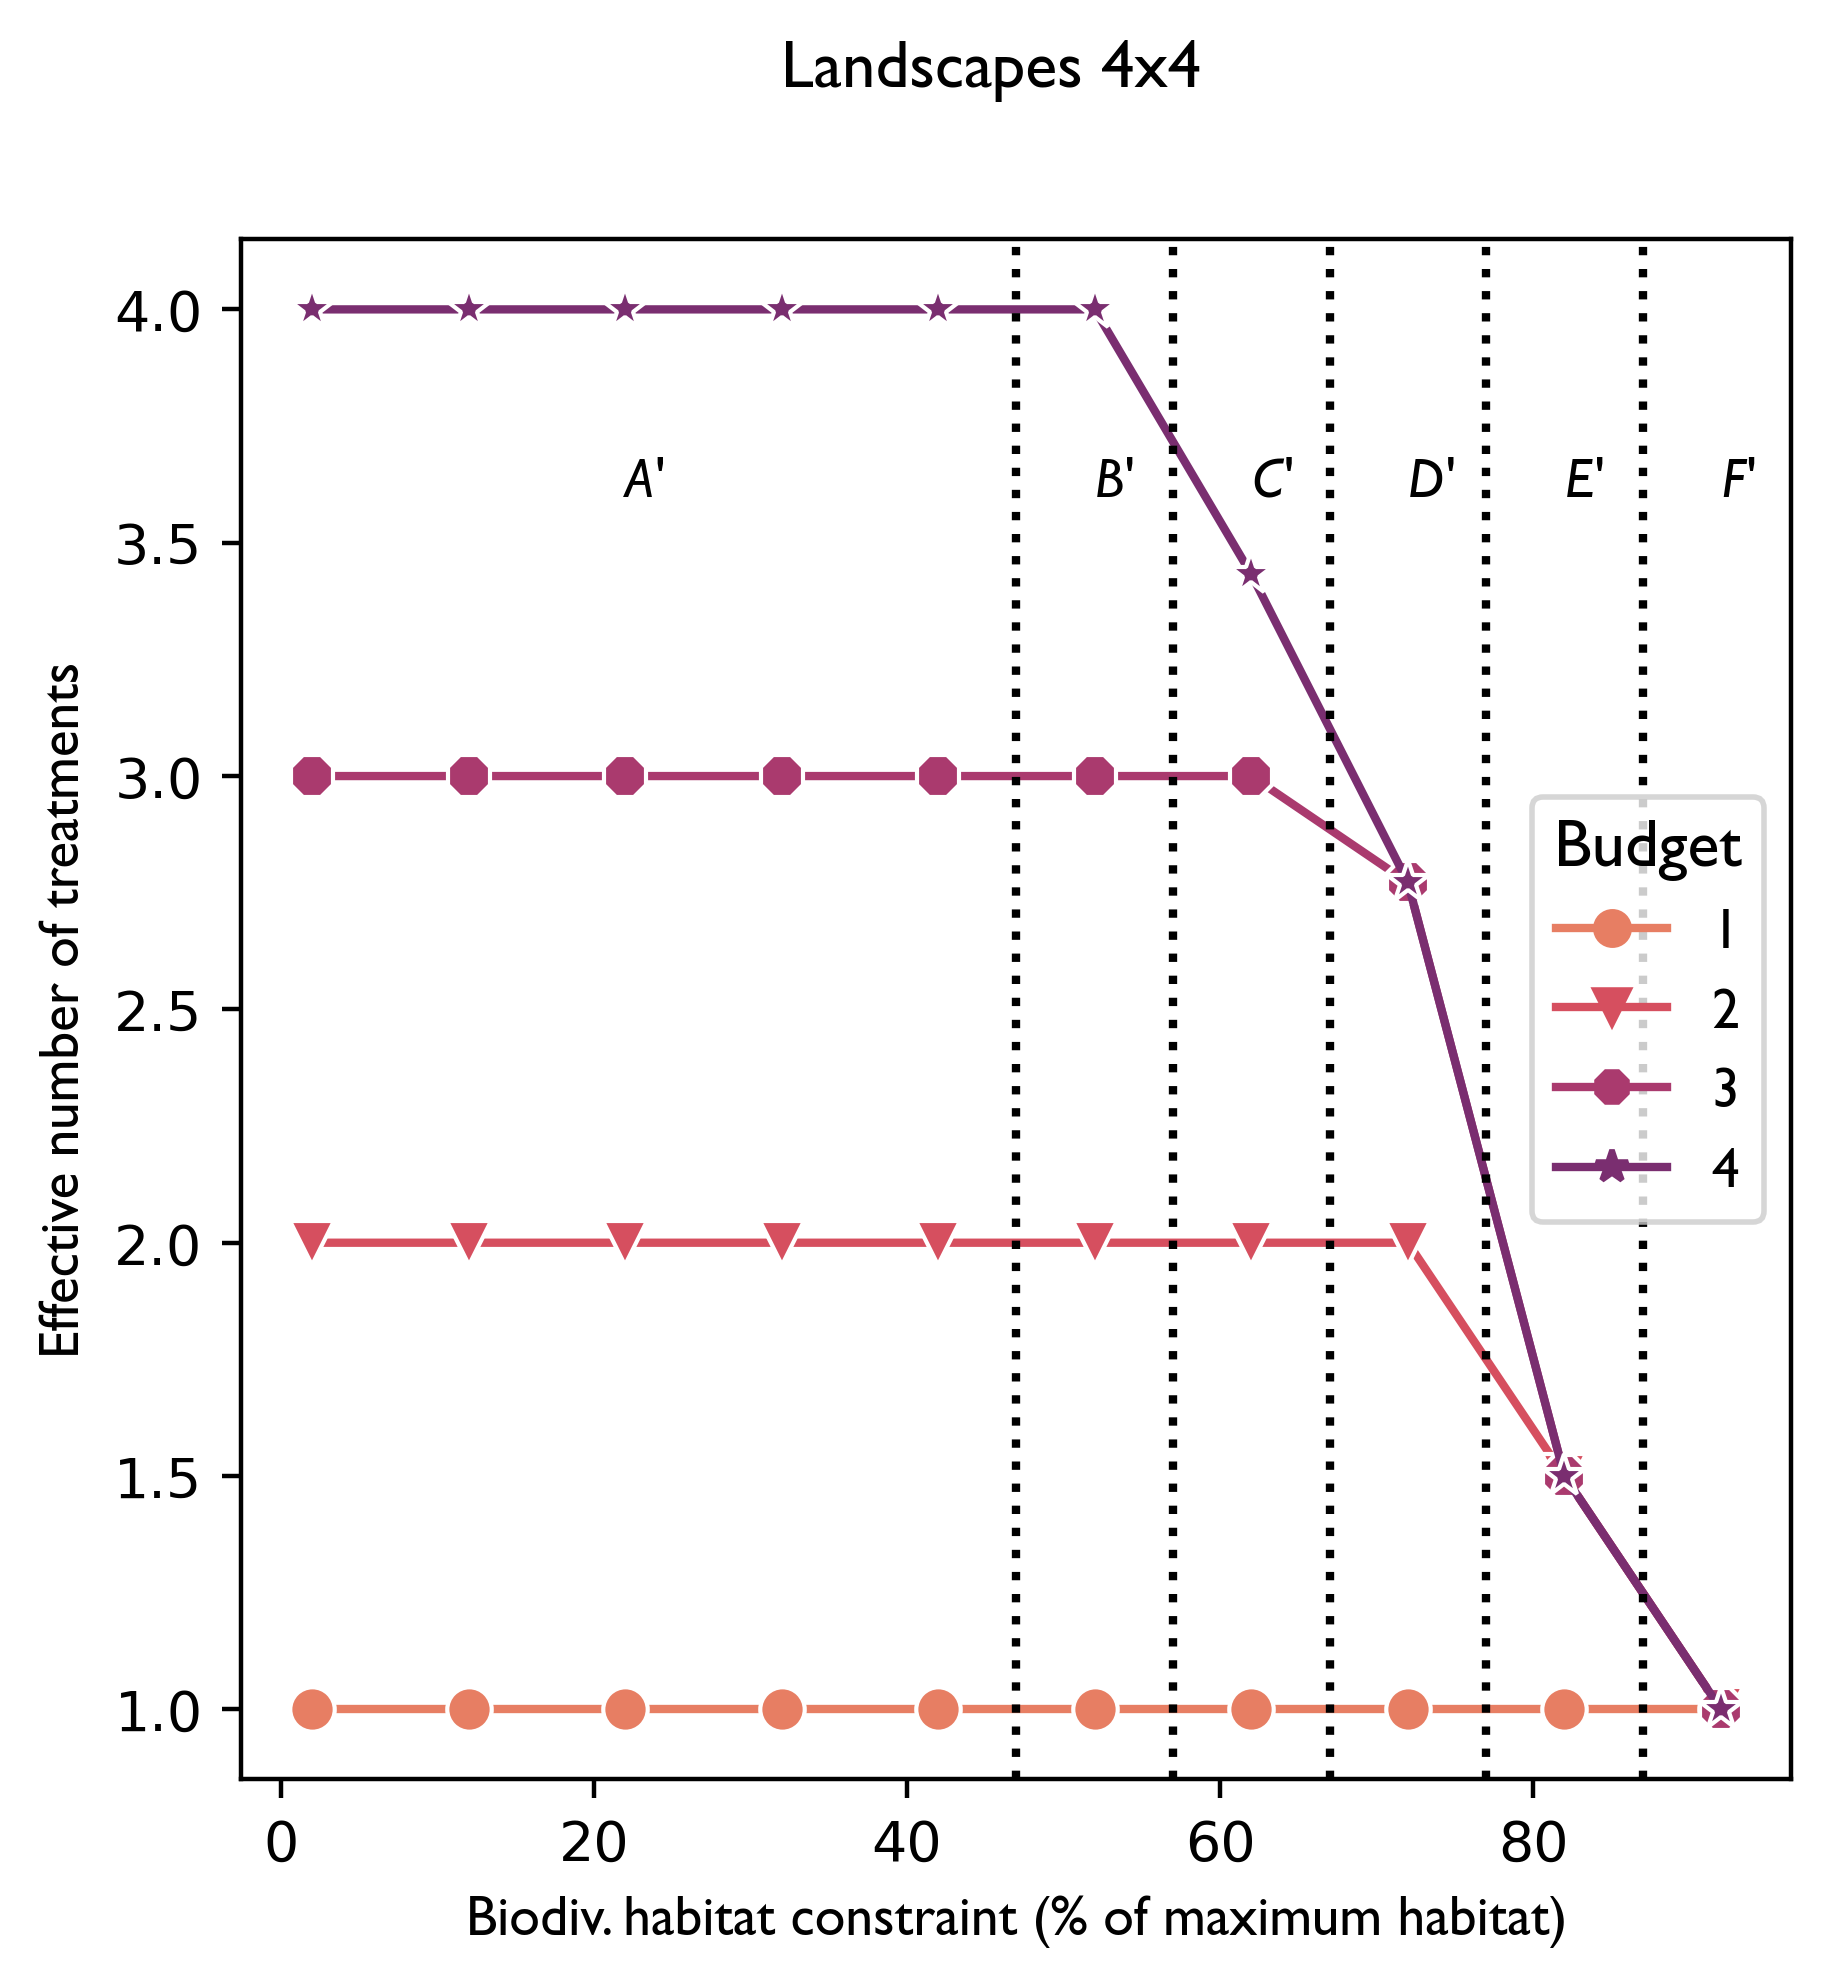
\includegraphics[width=\textwidth]{figures/wildland/number_treatments4.png}
%         \caption{}
%         \label{fig:treatments_number4}
%    \end{subfigure}
%    \hfill
%     \begin{subfigure}[b]{0.44\textwidth}
%         \centering
%         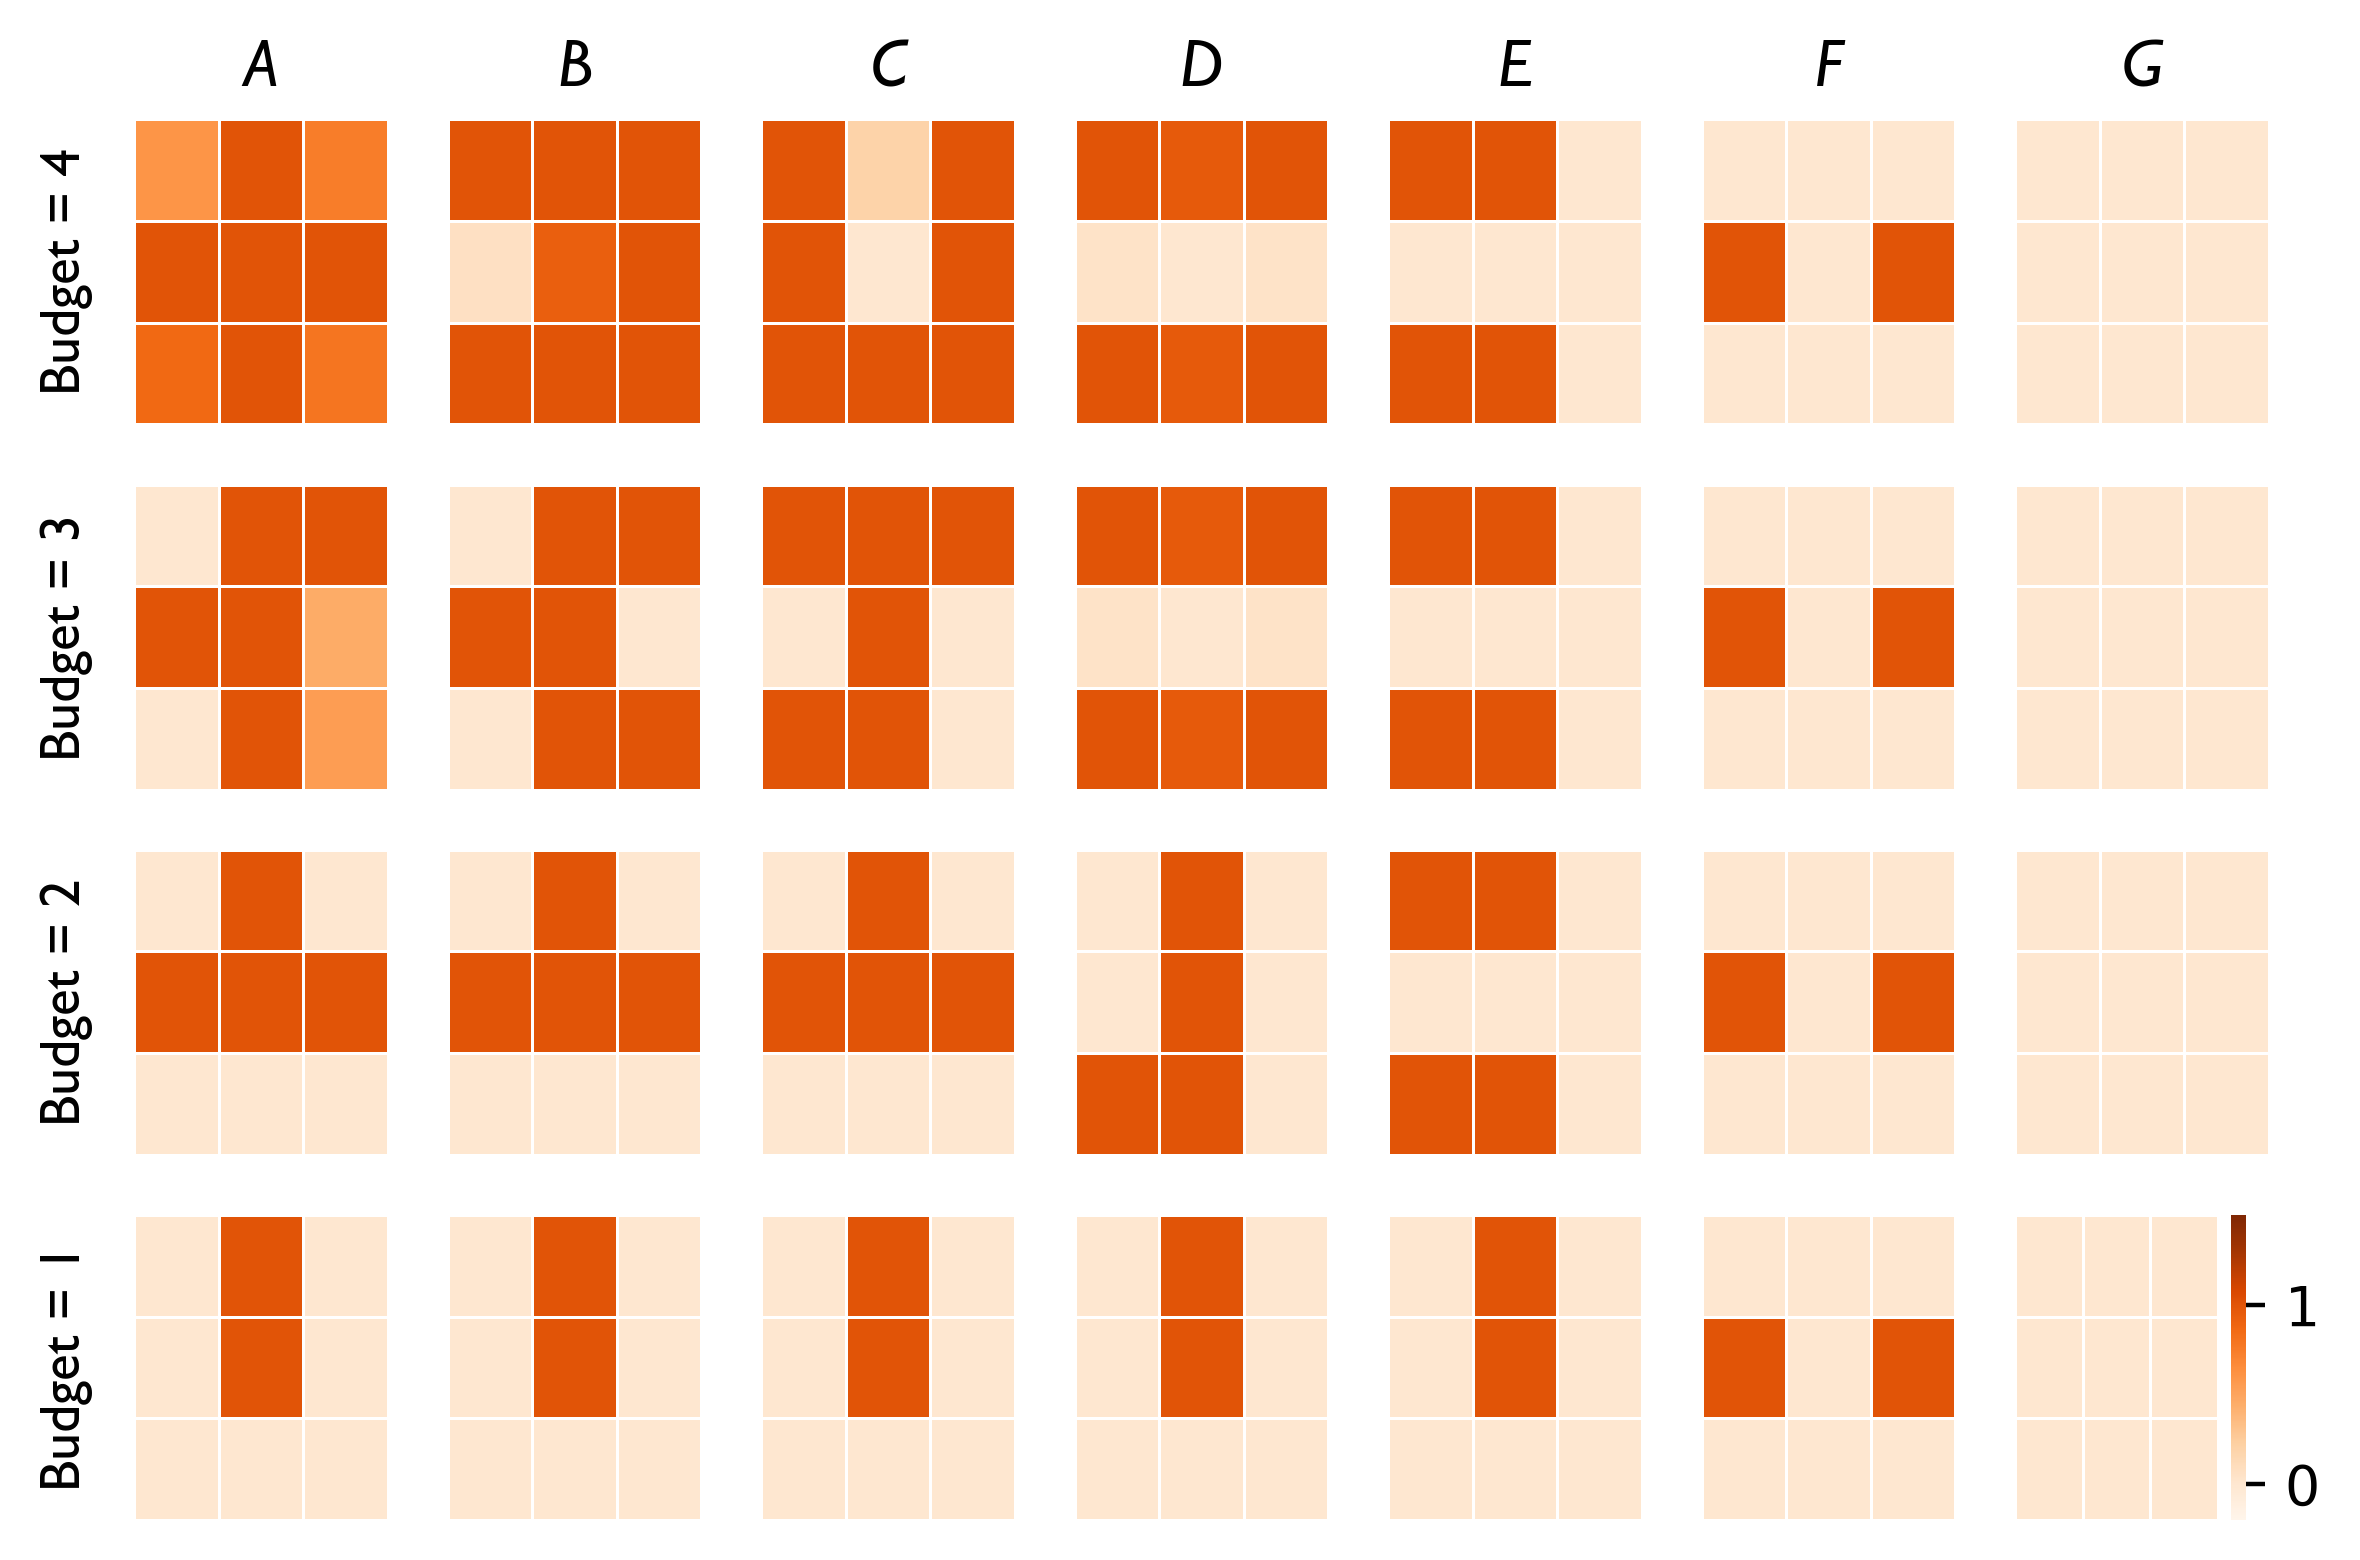
\includegraphics[width=\textwidth]{figures/wildland/treatments3.png}
%         \caption{}
%         \label{fig:treatments_pattern3}
%     \end{subfigure}
%     \begin{subfigure}[b]{0.44\textwidth}
%         \centering
%         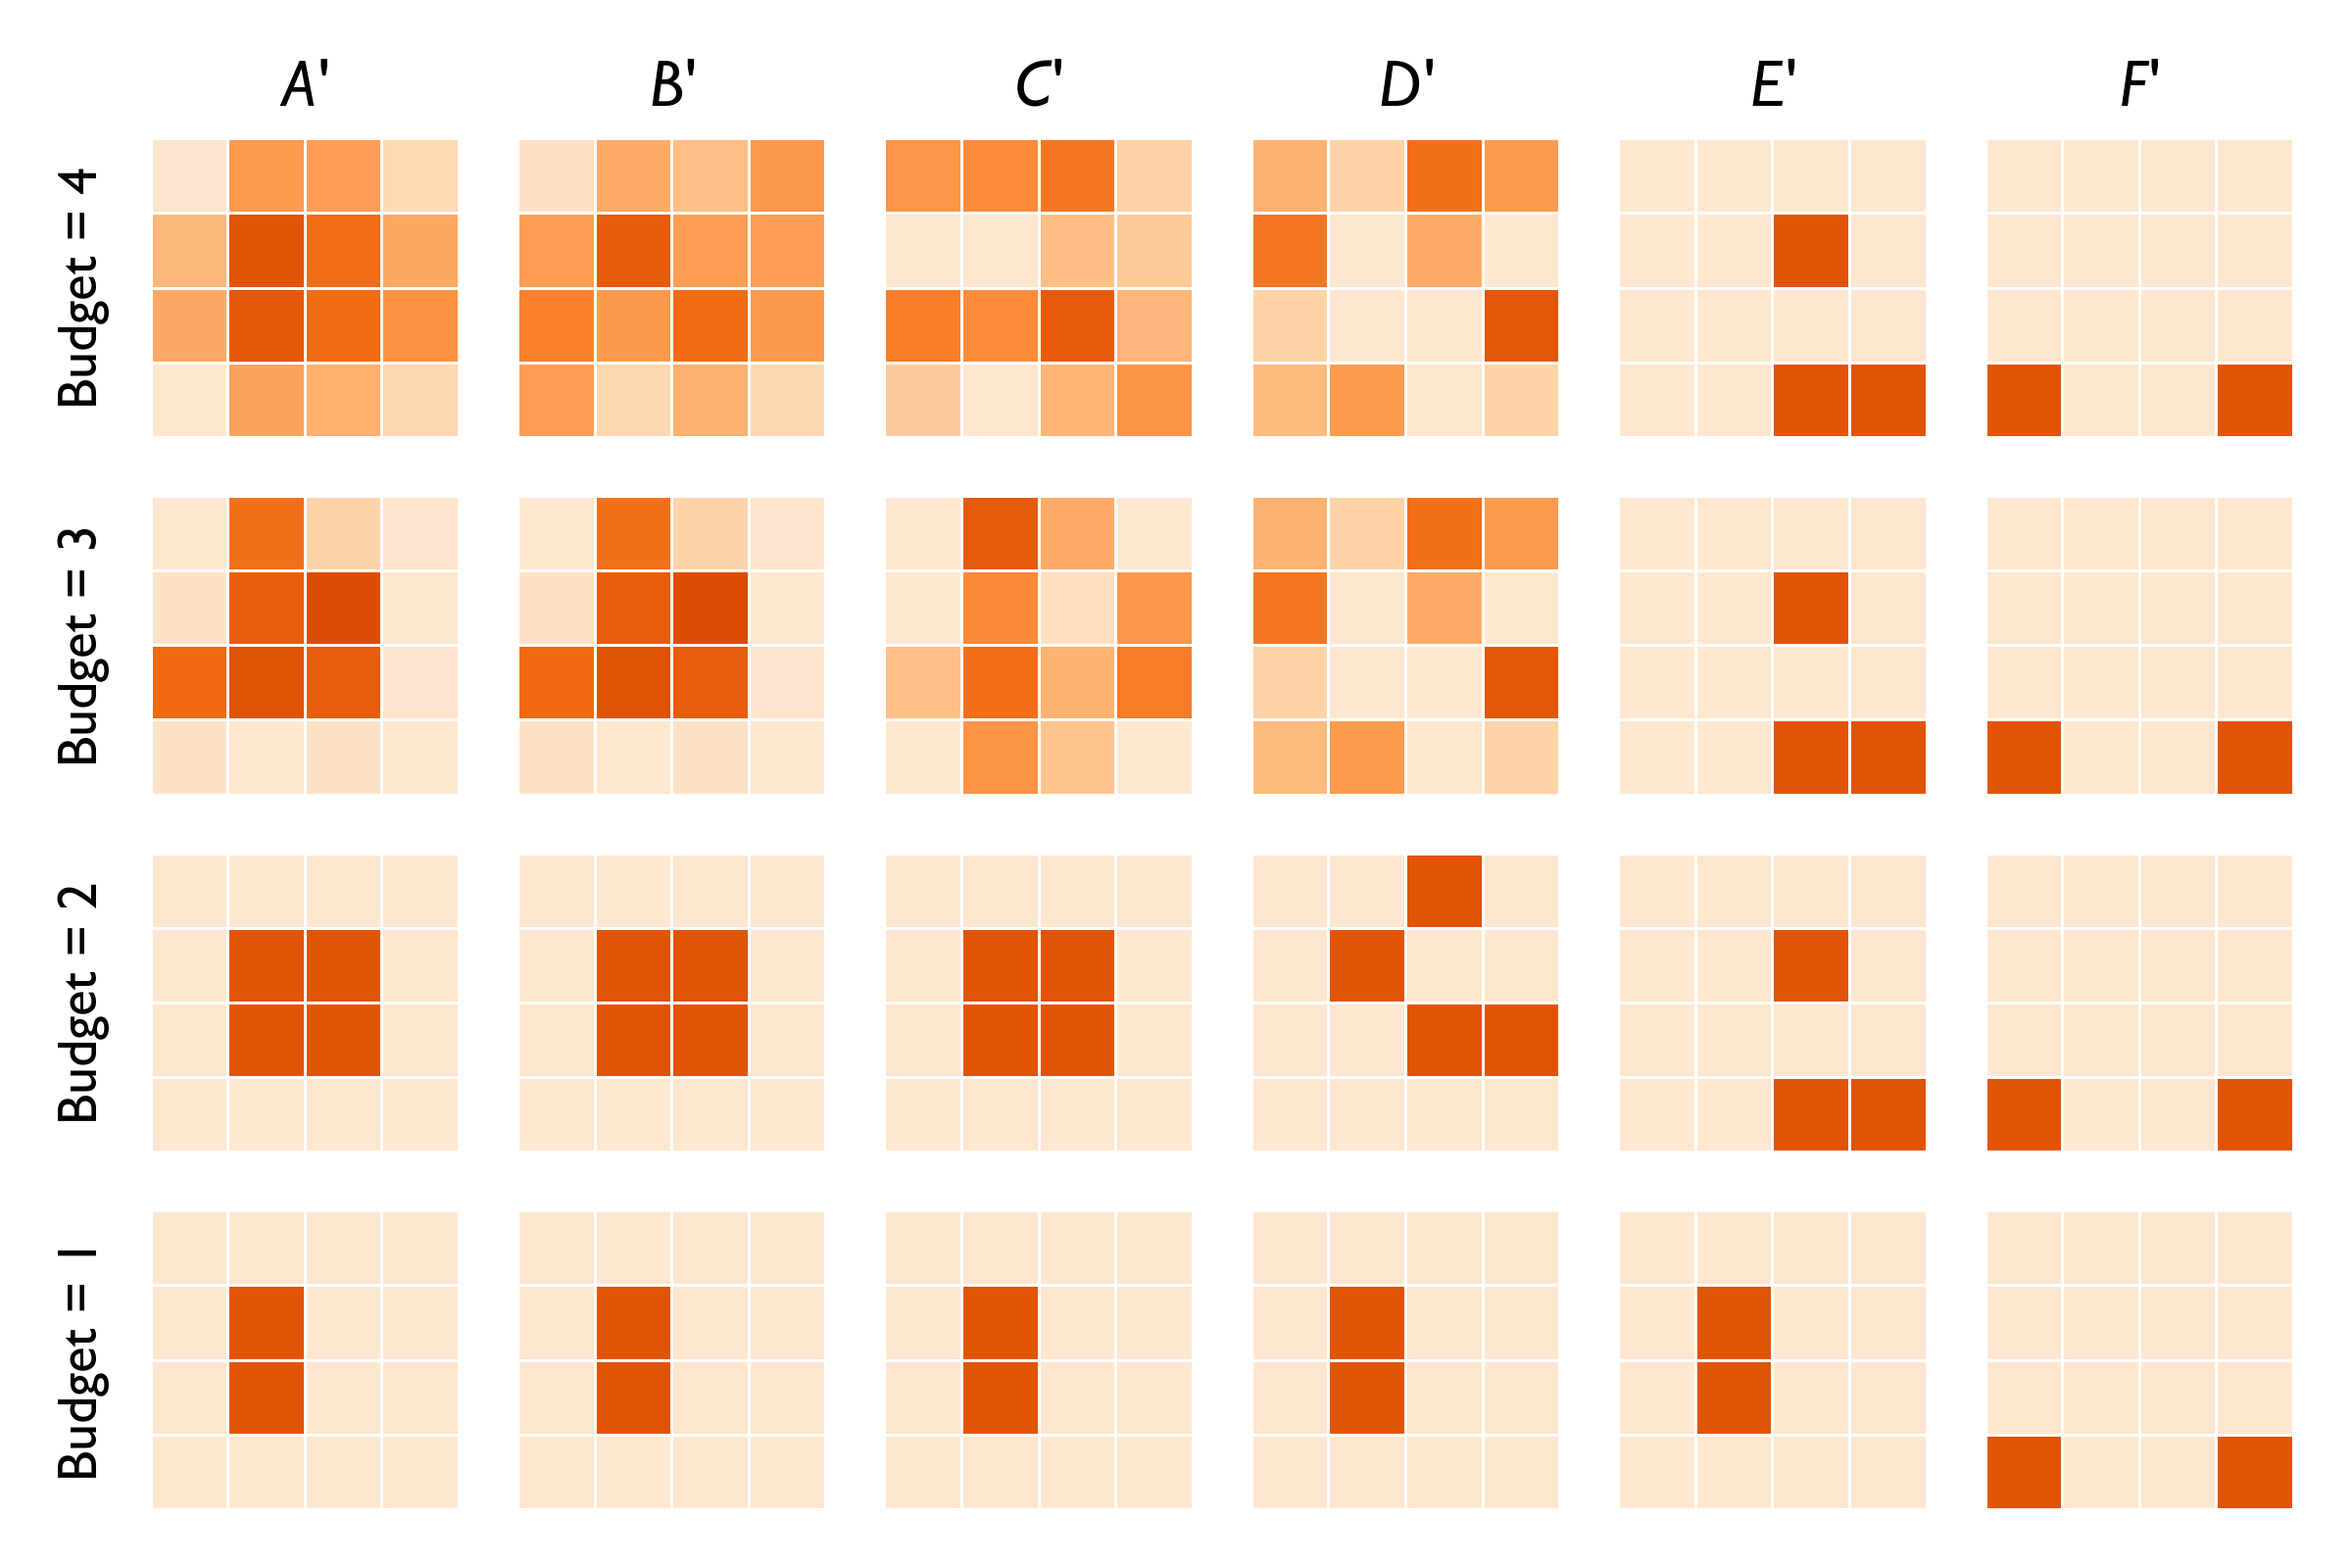
\includegraphics[width=\textwidth]{figures/wildland/treatments4.png}
%        \caption{}
%         \label{fig:treatments_pattern4}
%     \end{subfigure}    
%%        \caption{Treatment allocation : number, location}
%        \label{fig:treatments}
%\end{figure}

%\section{Tables}
%\begin{table}
%	\resizebox{.8\textwidth}{!}{
%	\centering
%	\begin{tabular}{|cc|ccc|ccc|ccc|ccc|}
%	& Budget & & 1 &  & & 2 &   & & 3 & & 4 &   & \\
%	\hline \hline
%	Biodiversity & &  &   & & & & & &  & &  & \\
%	Constraint & & Max & Min & Average & Max & Min & Average %& Max & Min & Average &Max & Min & Average\\
%	\hline \hline
%	2 & & 1 & 1 & 2 & 2 & 1 & 1 & 1 & 1 & 1 & 1 & 1.869884 & 1.826963\\
%	12 & & 1 & 1 & 2 & 2 & 1 & 1 & 1 & 1 & 1 & 1 & 1.869884 & 1.827013\\
%	22 & & 1 & 1 & 2 & 2 & 1 & 1 & 1 & 1 & 1 & 1 & 1.869884 & 1.827013\\
%	32 & & 1 & 1 & 2 & 2 & 1 & 1 & 1 & 1 & 1 & 1 & 1.869884 & 1.827013\\
%	42 & & 1 & 1 & 2 & 2 & 1 & 1 & 1 & 1 & 1 & 1 & 1.869884 & 1.827013\\
%	52 & & 1 & 1 & 2 & 2 & 1 & 1 & 1 & 1 & 1 & 1 & 1.869884 & 1.784694\\
%	62 & & 1 & 1 & 2 & 2 & 1 & 1 & 1 & 2 & 1 & 1 & 1.254153 & 2.000000\\
%	72 & & 1 & 2 & 2 & 2 & 1 & 2 & 1 & 1 & 1 & 2 & 1.428946 & 1.428922\\
%	82 & & 1 & 2 & 2 & 2 & 1 & 2 & 2 & 2 & 1 & 2 & 2.000000 & 2.000000\\
%	92 & & 1 & 1 & 1 & 1 & 1 & 1 & 1 & 1 & 1 & 1 & 1.000000 & 1.000000\\
%	\hline
%	\end{tabular}
%	}
%	\caption{Convergence periods for landscape cycles in steady state with size $n=4$}
%\end{table}
\clearpage

\subsection{Additional tables}
\label{sec:appendix_reg}
The main model is : 

\begin{align}
\label{model:simple}
DiffRisk_{i} &= \beta_0 + \beta_1 Budget_i + \beta_2 Constraint_i + \beta_3 Number2_i \\
&+ \beta_4 LSI_i + \beta_5 Simpson_i + \beta_6 SSHI_i + \beta_7 NumberComponents_i \notag \\
& + \beta_8 GlobalRiskInitial_i \notag
\end{align}

A second model is tested :

\begin{align}
\label{model:interacted}
DiffRisk_{i} &= \beta_0 + \beta_1 Budget_i + \beta_2 Constraint_i + \beta_3 LSI_i + \beta_4 Simpson_i \\
& + \beta_5 SSHI_i + \beta_6 GlobalRiskInitial_i + \beta_7 Constraint_i \times Budget_i \notag\\
& + \beta_8 LSI_i \times SSHI_i + \beta_9 LSI_i \times Simpson_i \notag\\
&  + \beta_{10}Constraint_i\times GlobalRiskInitial_i \notag \\
& + \beta_{10}Constraint_i\times GlobalRiskInitial_i \notag\\
& +\beta_{11}Budget_i\times GlobalRiskInitial_i \notag\\
& + \beta_{12} Constraint_i\times Budget_i \times GlobalRiskInitial_i \notag
\end{align}


\begin{table}[!htbp] \centering 
  \caption{Summary of model \ref{model:simple}: linear regression of risk differences between optimization procedures on landscape characteristics} 
  \label{tab:lm_risk} 
\begin{tabular}{@{\extracolsep{5pt}}lc} 
\\[-1.8ex]\hline 
\hline \\[-1.8ex] 
 & \multicolumn{1}{c}{\textit{Dependent variable:} } \\ 
\cline{2-2} 
\\[-1.8ex] & $DiffRisk_i$\\ 
\hline \\[-1.8ex] 
 Constraint & $-$0.009$^{***}$ \\ 
  & (0.001) \\ 
  & \\ 
 Budget & 0.753$^{***}$ \\ 
  & (0.030) \\ 
  & \\ 
 Number of 2s & 0.034 \\ 
  & (0.081) \\ 
  & \\ 
 LSI & $-$0.139 \\ 
  & (0.230) \\ 
  & \\ 
 Simpson & $-$0.654 \\ 
  & (0.618) \\ 
  & \\ 
 Successional Stage Heterogeneity Index & $-$0.990$^{**}$ \\ 
  & (0.490) \\ 
  & \\ 
 Number of components & $-$0.048 \\ 
  & (0.075) \\ 
  & \\ 
 Global Risk Connectiivty & 0.002 \\ 
  & (0.020) \\ 
  & \\ 
 Constant & 1.183$^{***}$ \\ 
  & (0.270) \\ 
  & \\ 
\hline \\[-1.8ex] 
Observations & 25,840 \\ 
R$^{2}$ & 0.028 \\ 
Adjusted R$^{2}$ & 0.027 \\ 
Residual Std. Error & 5.375 (df = 25831) \\ 
F Statistic & 91.470$^{***}$ (df = 8; 25831) \\ 
\hline 
\hline \\[-1.8ex] 
\textit{Note:}  & \multicolumn{1}{r}{$^{*}$p$<$0.1; $^{**}$p$<$0.05; $^{***}$p$<$0.01} \\ 
\end{tabular} 
\end{table} 



% Table created by stargazer v.5.2.3 by Marek Hlavac, Social Policy Institute. E-mail: marek.hlavac at gmail.com
% Date and time: jeu., sept. 05, 2024 - 17:45:31
\begin{table}[!htbp] \centering 
  \caption{Summary of model \ref{model:interacted}: linear regression of risk differences between optimization procedures on landscape characteristics } 
  \label{} 
\resizebox{\textwidth}{!}{%
\begin{tabular}{@{\extracolsep{5pt}}lc} 
\\[-1.8ex]\hline 
\hline \\[-1.8ex] 
 & \multicolumn{1}{c}{\textit{Dependent variable:}} \\ 
\cline{2-2} 
\\[-1.8ex] & $DiffRisk_i$ \\ 
\hline \\[-1.8ex] 
 Constraint & $-$0.008$^{*}$ \\ 
  & (0.005) \\ 
  & \\ 
 Budget & 0.661$^{***}$ \\ 
  & (0.108) \\ 
  & \\ 
 LSI & 0.584 \\ 
  & (0.643) \\ 
  & \\ 
 Succesional Stage Heterogeneity Index (SSHI) & 1.087 \\ 
  & (2.203) \\ 
  & \\ 
 Simpson & $-$1.612 \\ 
  & (2.532) \\ 
  & \\ 
 Global Risk Connectivity & $-$0.022 \\ 
  & (0.023) \\ 
  & \\ 
 Constraint $\times$ Budget & 0.0002 \\ 
  & (0.002) \\ 
  & \\ 
 LSI $\times$ SSHI & $-$1.446 \\ 
  & (1.605) \\ 
  & \\ 
 LSI $\times$ Simpson & 0.201 \\ 
  & (2.018) \\ 
  & \\ 
 Constraint $\times$ Global Risk Connectivity & 0.0002 \\ 
  & (0.0004) \\ 
  & \\ 
 Budget$\times$ Global Risk Connectivity  & 0.017$^{**}$ \\ 
  & (0.009) \\ 
  & \\ 
Cconstraint $\times$ Budget$\times$ Global Risk Connectivity  & $-$0.0002 \\ 
  & (0.0001) \\ 
  & \\ 
 Constant & 0.662 \\ 
  & (0.647) \\ 
  & \\ 
\hline \\[-1.8ex] 
Observations & 25,840 \\ 
R$^{2}$ & 0.028 \\ 
Adjusted R$^{2}$ & 0.027 \\ 
Residual Std. Error & 5.375 (df = 25827) \\ 
F Statistic & 61.872$^{***}$ (df = 12; 25827) \\ 
\hline 
\hline \\[-1.8ex] 
\textit{Note:}  & \multicolumn{1}{r}{$^{*}$p$<$0.1; $^{**}$p$<$0.05; $^{***}$p$<$0.01} \\ 
\end{tabular}
}
\end{table} 

\cleardoublepage